\documentclass[xcolor={svgnames}]{beamer}


% PACKAGES 
% ========

% Do not indent paragraphs and insert blank space between paragraphs.
\usepackage{parskip}

% To enter link, GitHub, and Twitter icons.
\usepackage{fontawesome}

% Commands like \textasciigrave, \textquotesingle, etc. are required by
% listings when \lstset{upquote=true} is used. They are defined in
% textcomp.sty.
\usepackage{textcomp}

% To enter syntax-highlighted code blocks.
\usepackage{listings}

% To use \toprule in tabular environment.
\usepackage{booktabs}

% To use \arraybackslash in new columntype definition for tabular.
\usepackage{array}


% THEME
% =====

% Set main theme.
\usetheme{CambridgeUS}

% Set outer color theme.
\usecolortheme{dolphin}

% Set inner color theme for blocks.
\usecolortheme{orchid}

% Remove navigation symbols from footer.
\setbeamertemplate{navigation symbols}{}

% CambridgeUS uses infolines.sty for outer theme which in turn defines
% footline with three color boxes for author, title, and date. We set
% the footline to omit the color box for title and distribute the width
% of the remaining two color boxes equally across the paper width. The
% code below is a derivative of the \defbeamertemplate*{footline} code
% in infolines.sty.
\setbeamertemplate{footline}
{%
  \leavevmode%
  \hbox{%
  \begin{beamercolorbox}[wd=.5\paperwidth,ht=2.25ex,dp=1ex,center]
        {author in head/foot}%
    \usebeamerfont{author in head/foot}\insertshortauthor
                  {~~~~(\insertshortinstitute)}
  \end{beamercolorbox}%
  \begin{beamercolorbox}[wd=.5\paperwidth,ht=2.25ex,dp=1ex,right]
        {date in head/foot}%
    \usebeamerfont{date in head/foot}\insertshortdate{}\hspace*{2em}
    \usebeamertemplate{page number in head/foot}\hspace*{2ex} 
  \end{beamercolorbox}}%
  \vskip0pt%
}


% LINKS
% =====

% Color links blue.
\hypersetup{colorlinks=true,urlcolor=blue}

% Use current text font for links (override default teletype font).
\urlstyle{same}


% CODE LISTINGS
% =============

\lstdefinestyle{plain}{
    basicstyle=\ttfamily\color{DarkBlue},
    columns=fullflexible,
    keepspaces=true,
    upquote=true,
    showlines=true,
    moredelim=[is][\color{DarkBlue}]{<<}{>>},
    moredelim=[is][\color{Gray}]{~~}{~~},
    moredelim=[is][\color{Red}]{!!}{!!},
    moredelim=[is][\color{Green}]{++}{++},
}

\lstdefinestyle{color}{
    showstringspaces=false,
    commentstyle=\color{DarkGreen},
    keywordstyle=\color{Blue},
    identifierstyle=\color{Indigo},
    stringstyle=\color{Maroon},
}

\lstdefinestyle{python}{
    language=python,
    style=plain,
    style=color,
    morekeywords={as},
    moredelim=[is][\color{Gray}\sout]{\#\ --}{--},
}

\lstdefinestyle{shell}{
    language=sh,
    style=plain,
    commentstyle=\color{DarkGreen},
}

\lstdefinestyle{small}{basicstyle=\small\ttfamily\color{DarkBlue}}
\lstdefinestyle{footnotesize}{basicstyle=\footnotesize\ttfamily\color{DarkBlue}}
\lstdefinestyle{scriptsize}{basicstyle=\scriptsize\ttfamily\color{DarkBlue}}
\lstdefinestyle{tiny}{basicstyle=\tiny\ttfamily\color{DarkBlue}}

\lstnewenvironment{pyenv}[1][]{\lstset{style=python,style=small,#1}}{}
\lstnewenvironment{shenv}[1][]{\lstset{style=shell,style=small,#1}}{}

\newcommand{\ttcode}[2][]{\lstinline[style=plain,basicstyle=\ttfamily#1]{#2}}
\newcommand{\pycode}[2][]{\lstinline[style=python,#1]{#2}}
\newcommand{\pyfile}[2][]{\lstinputlisting[style=python,style=small,#1]{#2}}


% TITLE PAGE METADATA
% ===================

\title{A Tour of Matplotlib}
\subtitle{\texorpdfstring{\vspace{2mm}}{}From Bar Charts to XKCD-Style Plots}
\author{Susam Pal}
\institute[PyCon UK 2019, Cardiff, UK]{
    PyCon UK 2019, Cardiff City Hall, Cardiff, UK
}
\date{15 Sep 2019}


% SLIDES
% ======

\begin{document}

\iftrue

% Title
\frame{\titlepage}


% About Me
\begin{frame}[t]
    \frametitle{About Me}

    Security architect at Walmart Labs.

    Developing security services in Python and Go.

    Author of a few open source projects:

        \qquad \faCodeFork{} \makebox[13mm][l]{TeXMe:}
        \url{https://github.com/susam/texme}

        \qquad \faCodeFork{} \makebox[13mm][l]{GitPR:}
        \url{https://github.com/susam/gitpr}

        \qquad \faCodeFork{} \makebox[13mm][l]{Uncap:}
        \url{https://github.com/susam/uncap}

    Websites:

        \qquad \faTwitter{} \url{https://twitter.com/susam}

        \qquad \faGithub{} \url{https://github.com/susam}

        \qquad \faLink{} \url{https://susam.in/}

\end{frame}


% Get Started
\begin{frame}[t,fragile]
    \frametitle{Get Started}
    \vspace{5mm}
    \begin{columns}[T]
        \begin{column}{0.52\textwidth}
            \begin{onlyenv}<1->
                \begin{shenv}[gobble=20]
                    $ python3 -m venv myenv
                    $ source myenv/bin/activate
                    $ pip3 install matplotlib
                \end{shenv}
            \end{onlyenv}
            \begin{onlyenv}<2->
                \begin{pyenv}[gobble=20]
                    <<$ python3>>
                    >>> import matplotlib.pyplot as plt
                    >>> plt.plot([2, 3, 5, 7, 11])
                    >>> plt.show()
                \end{pyenv}
            \end{onlyenv}
        \end{column}
        \begin{column}{0.48\textwidth}
            \includegraphics<3>[width=\textwidth]{img/00-setup.png}
        \end{column}
    \end{columns}
\end{frame}


% Save Plot to File
\begin{frame}
    \frametitle{Save Plot to File}
    \begin{columns}
        \begin{column}{0.52\textwidth}
            \pyfile[linerange={1-4}]{examples/01-savefig.py}
        \end{column}
        \begin{column}{0.48\textwidth}
            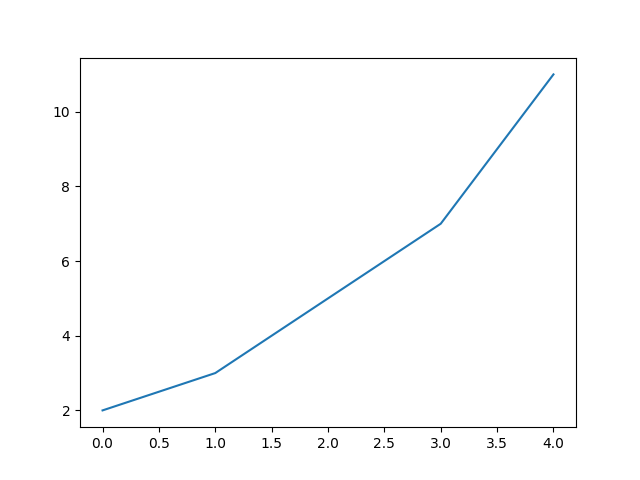
\includegraphics[width=\textwidth]{img/01-savefig-dpi-none.png}
        \end{column}
    \end{columns}
    \small
    \vspace{15mm}
    \hspace{-1.97mm}
    The default DPI (dots per inch) used to save the image is 100.
\end{frame}


% DPI: File Size vs. Quality Tradeoff
\begin{frame}
    \frametitle{DPI: File Size vs. Quality Tradeoff}
    \vspace{1.5mm}
    \newcolumntype{C}{>{\centering\arraybackslash} m{19.5mm}}
    \begin{tabular}{CCCCC}
        \toprule
        \textbf{DPI} & \textbf{Inches} & \textbf{Pixels} & \textbf{KB}
            & \textbf{Quality} \\
        \toprule

        100 & 6.4" x 4.8" &  640 x  480 &  15 KB  &
            
\includegraphics[height=9mm]{img/digit-dpi-100.png} \\
            \midrule

        200 & 6.4" x 4.8" & 1280 x  960 &  34 KB  &
            
\includegraphics[height=9mm]{img/digit-dpi-200.png} \\
            \midrule

        300 & 6.4" x 4.8" & 1920 x 1440 &  57 KB &
            
\includegraphics[height=9mm]{img/digit-dpi-300.png} \\
            \midrule

        400 & 6.4" x 4.8" & 2560 x 1920 &  78 KB &
            
\includegraphics[height=9mm]{img/digit-dpi-400.png} \\
            \midrule

        500 & 6.4" x 4.8" & 3200 x 2400 & 104 KB &
            
\includegraphics[height=9mm]{img/digit-dpi-500.png} \\

        \bottomrule
    \end{tabular}
\end{frame}


% Save Plot to a File: Set DPI to 300
\begin{frame}
    \frametitle{Save Plot to File: Set DPI to 300}
    \begin{columns}
        \begin{column}{0.52\textwidth}
            \pyfile[linerange={1-3,5-5}]{examples/01-savefig.py}
        \end{column}
        \begin{column}{0.48\textwidth}
            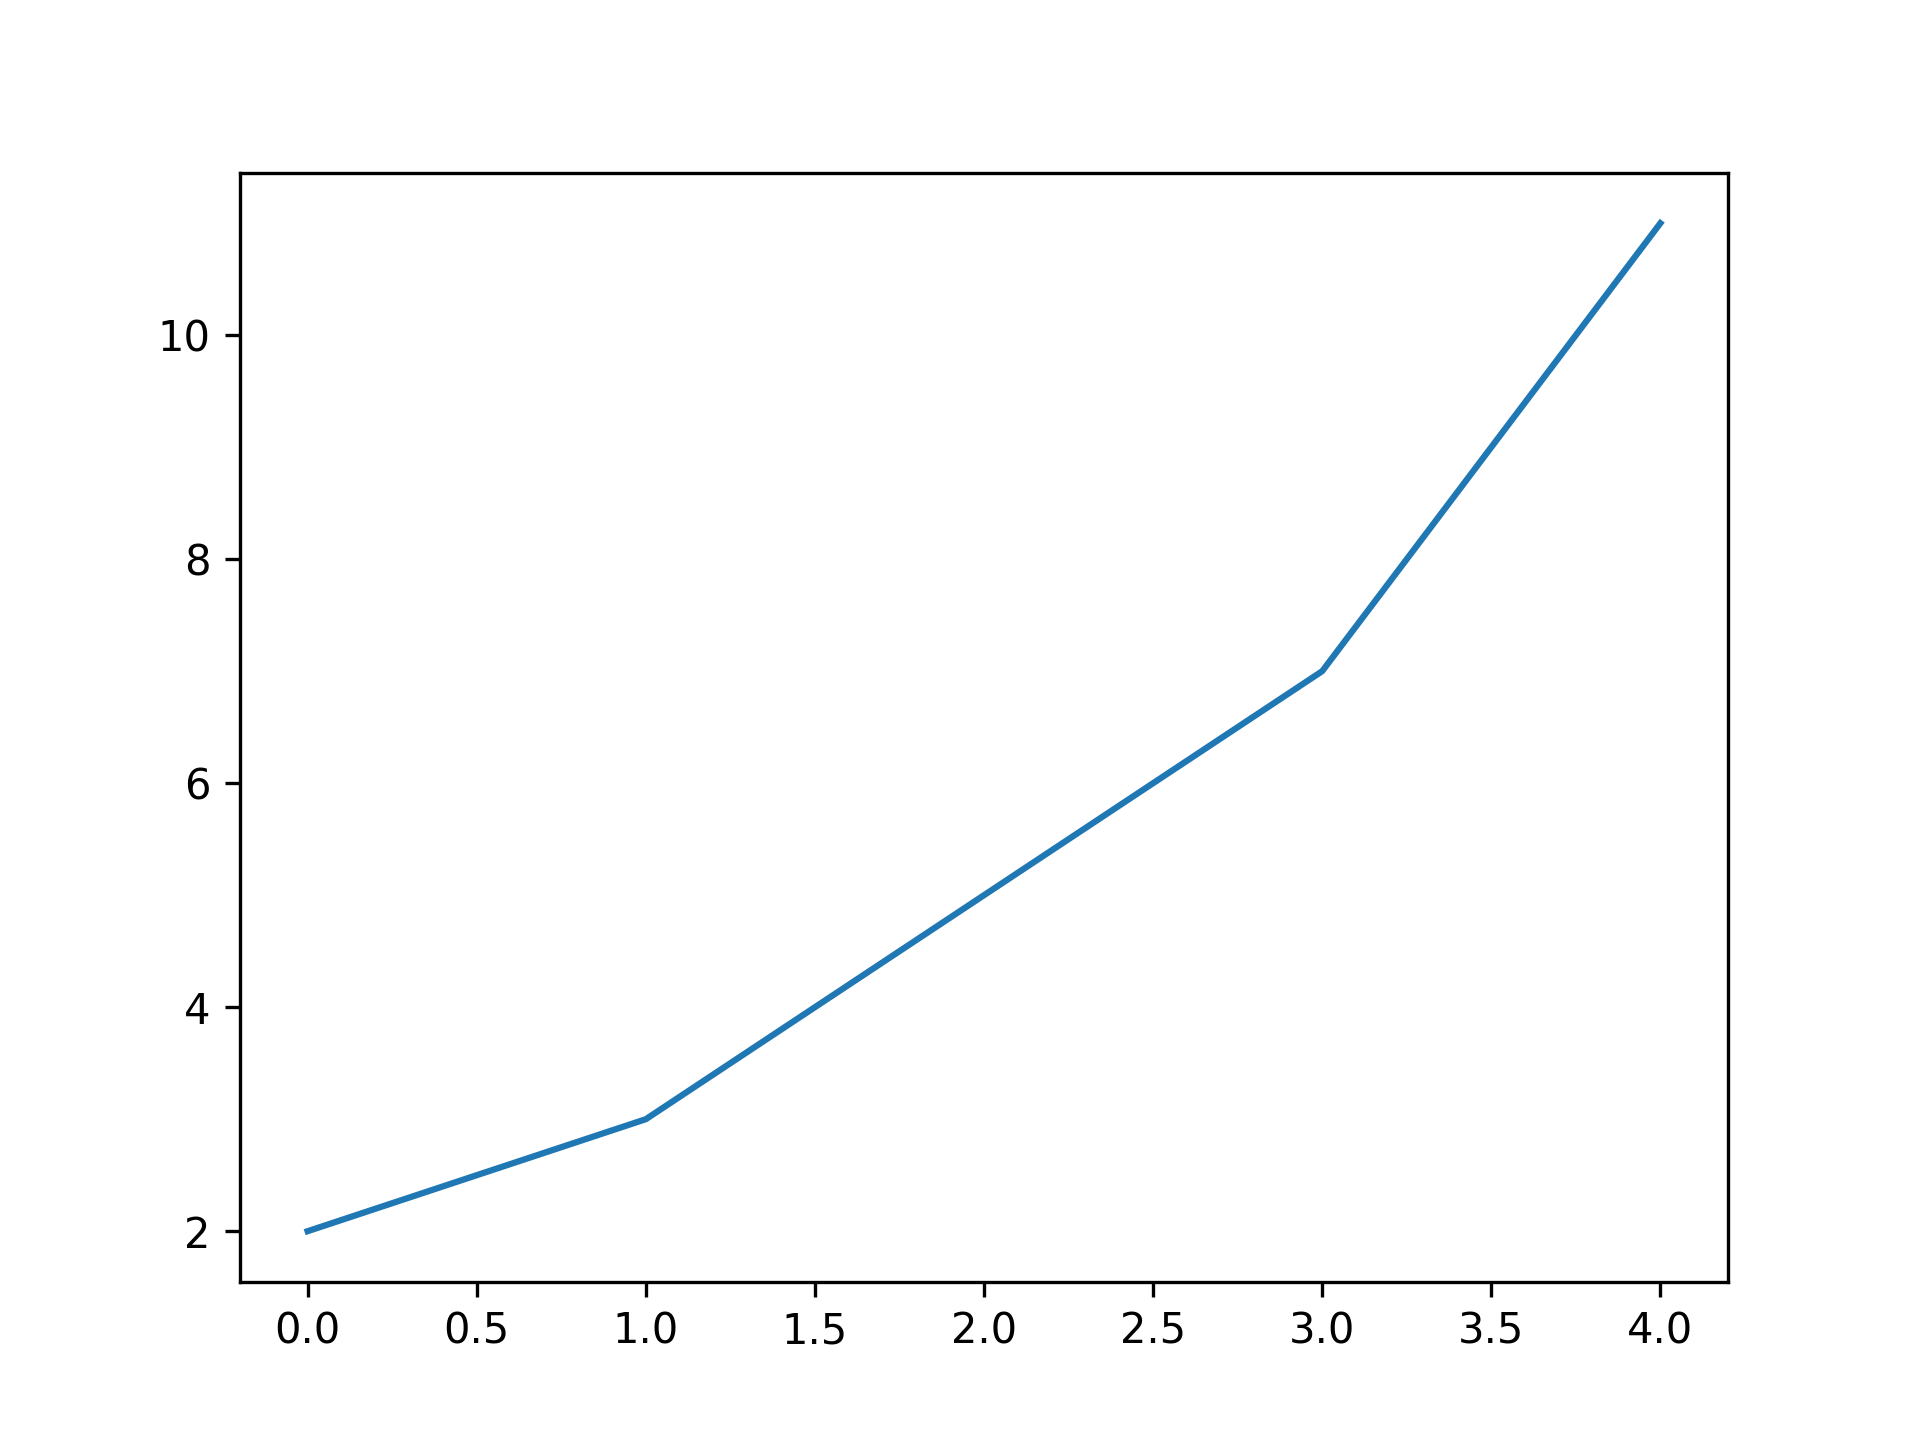
\includegraphics[width=\textwidth]{img/02-savefig-dpi-300.png}
        \end{column}
    \end{columns}
    \small
    \vspace{15mm}
    \hspace{-1.97mm}
    DPI value of 300 provides a good tradeoff between quality
    and file size.
\end{frame}


% Default Bounding Box
\begin{frame}[fragile]
    \frametitle{Default Bounding Box}
    \begin{columns}
        \begin{column}{0.52\textwidth}
            \pyfile[linerange={1-3,5-5}]{examples/01-savefig.py}
        \end{column}
        \begin{column}{0.48\textwidth}
            \frame{
                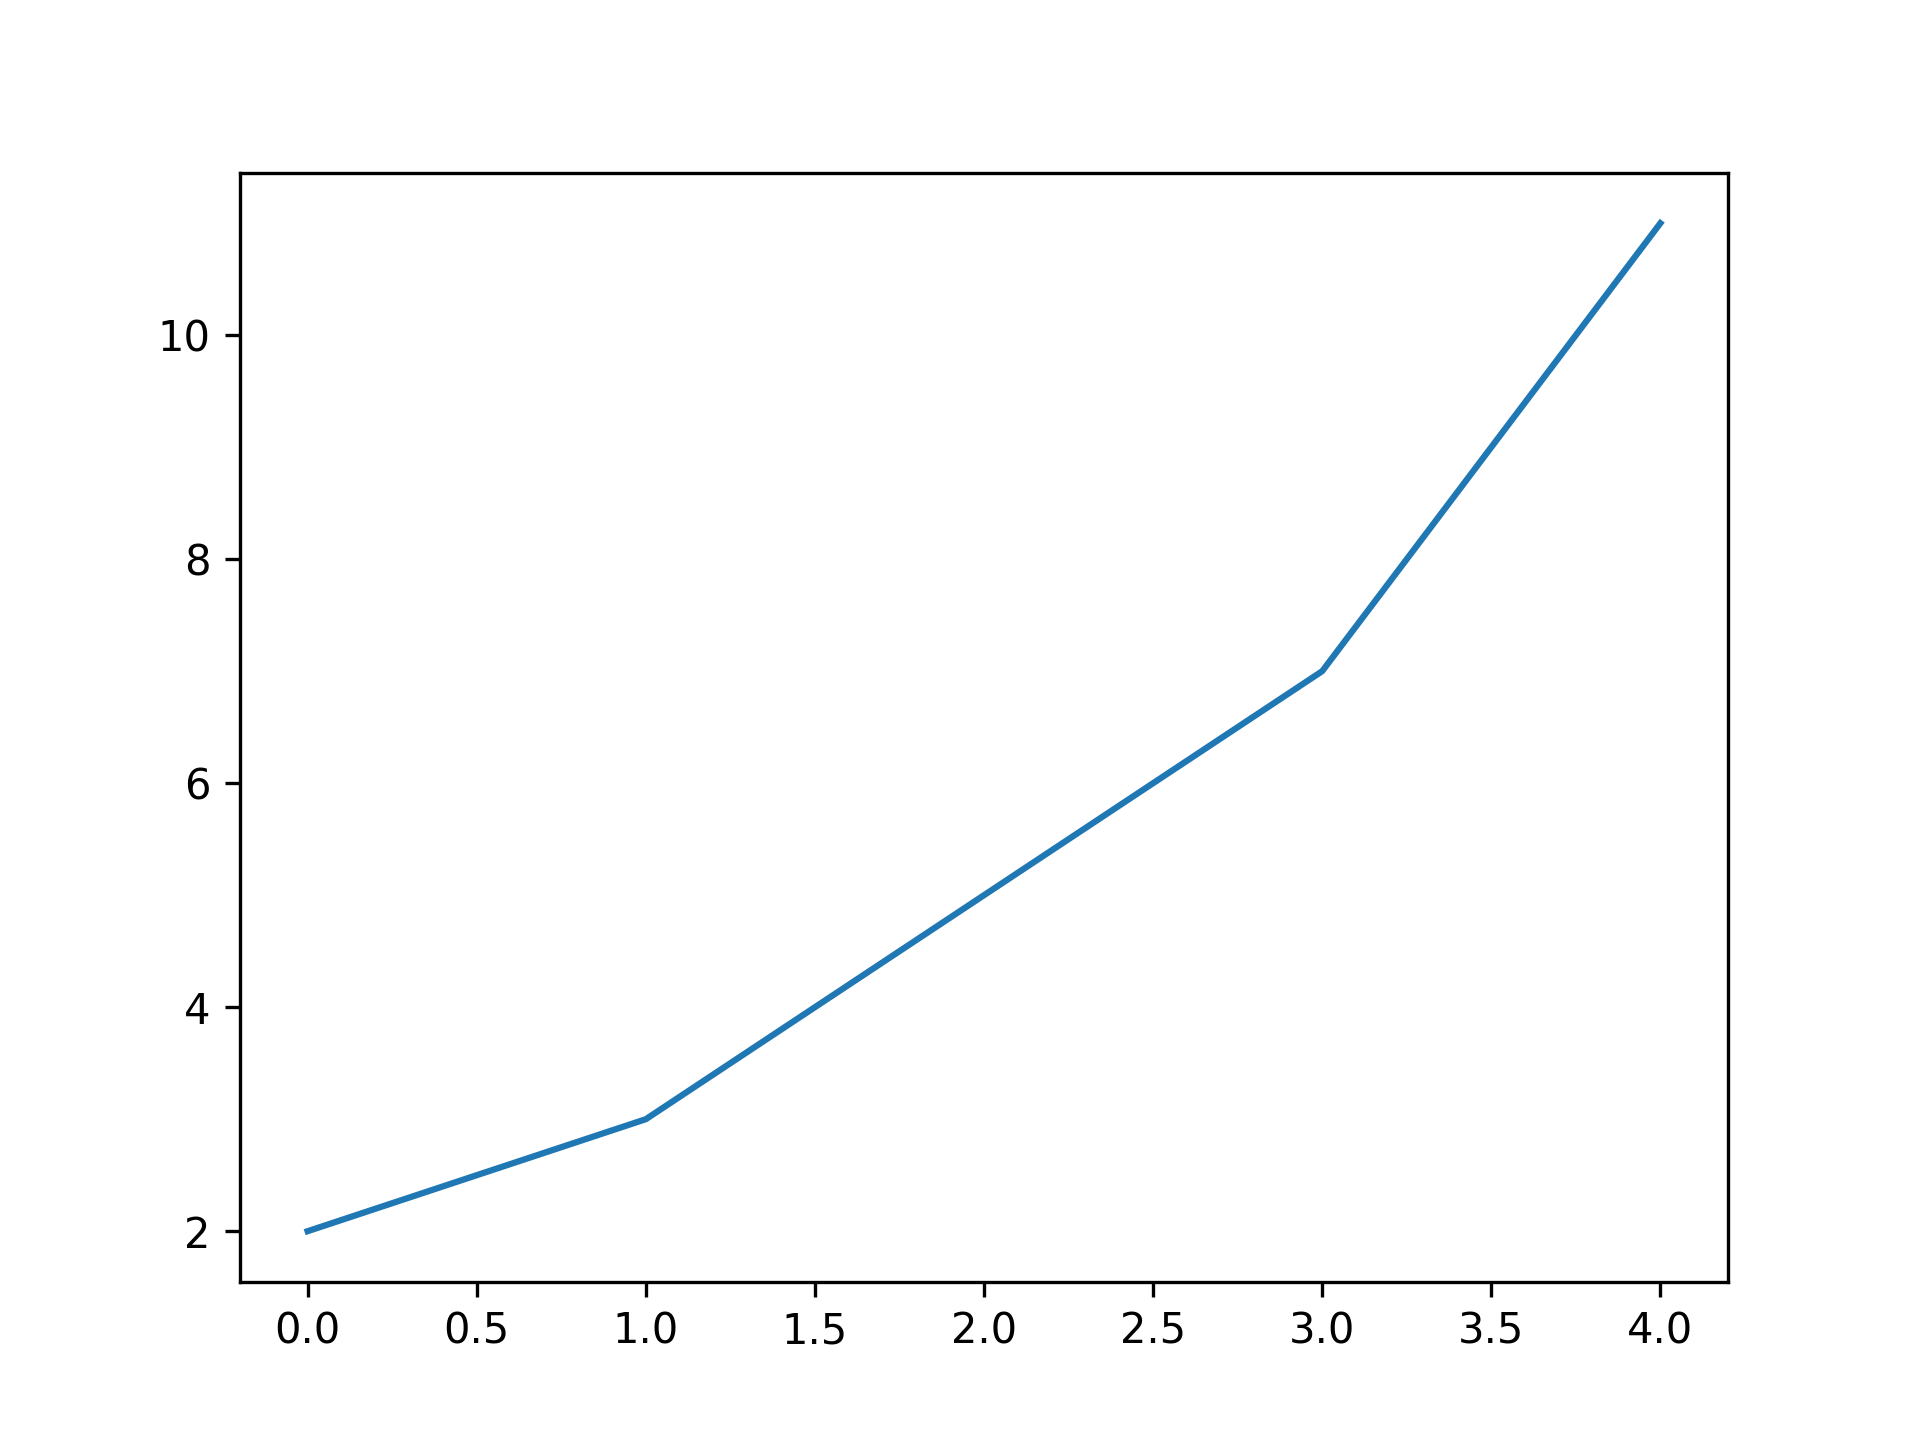
\includegraphics[width=\textwidth]{img/02-savefig-dpi-300.png}
            }
        \end{column}
    \end{columns}
    \small
    \vspace{15mm}
    \hspace{-1.97mm}
    By default there is a lot of padding around the plot. The bounding
    box is large.
\end{frame}


% Tight Bounding Box
\begin{frame}[fragile]
    \frametitle{Tight Bounding Box}
    \begin{columns}
        \begin{column}{0.52\textwidth}
            \pyfile{examples/03-savefig-tight.py}
        \end{column}
        \begin{column}{0.48\textwidth}
            \frame{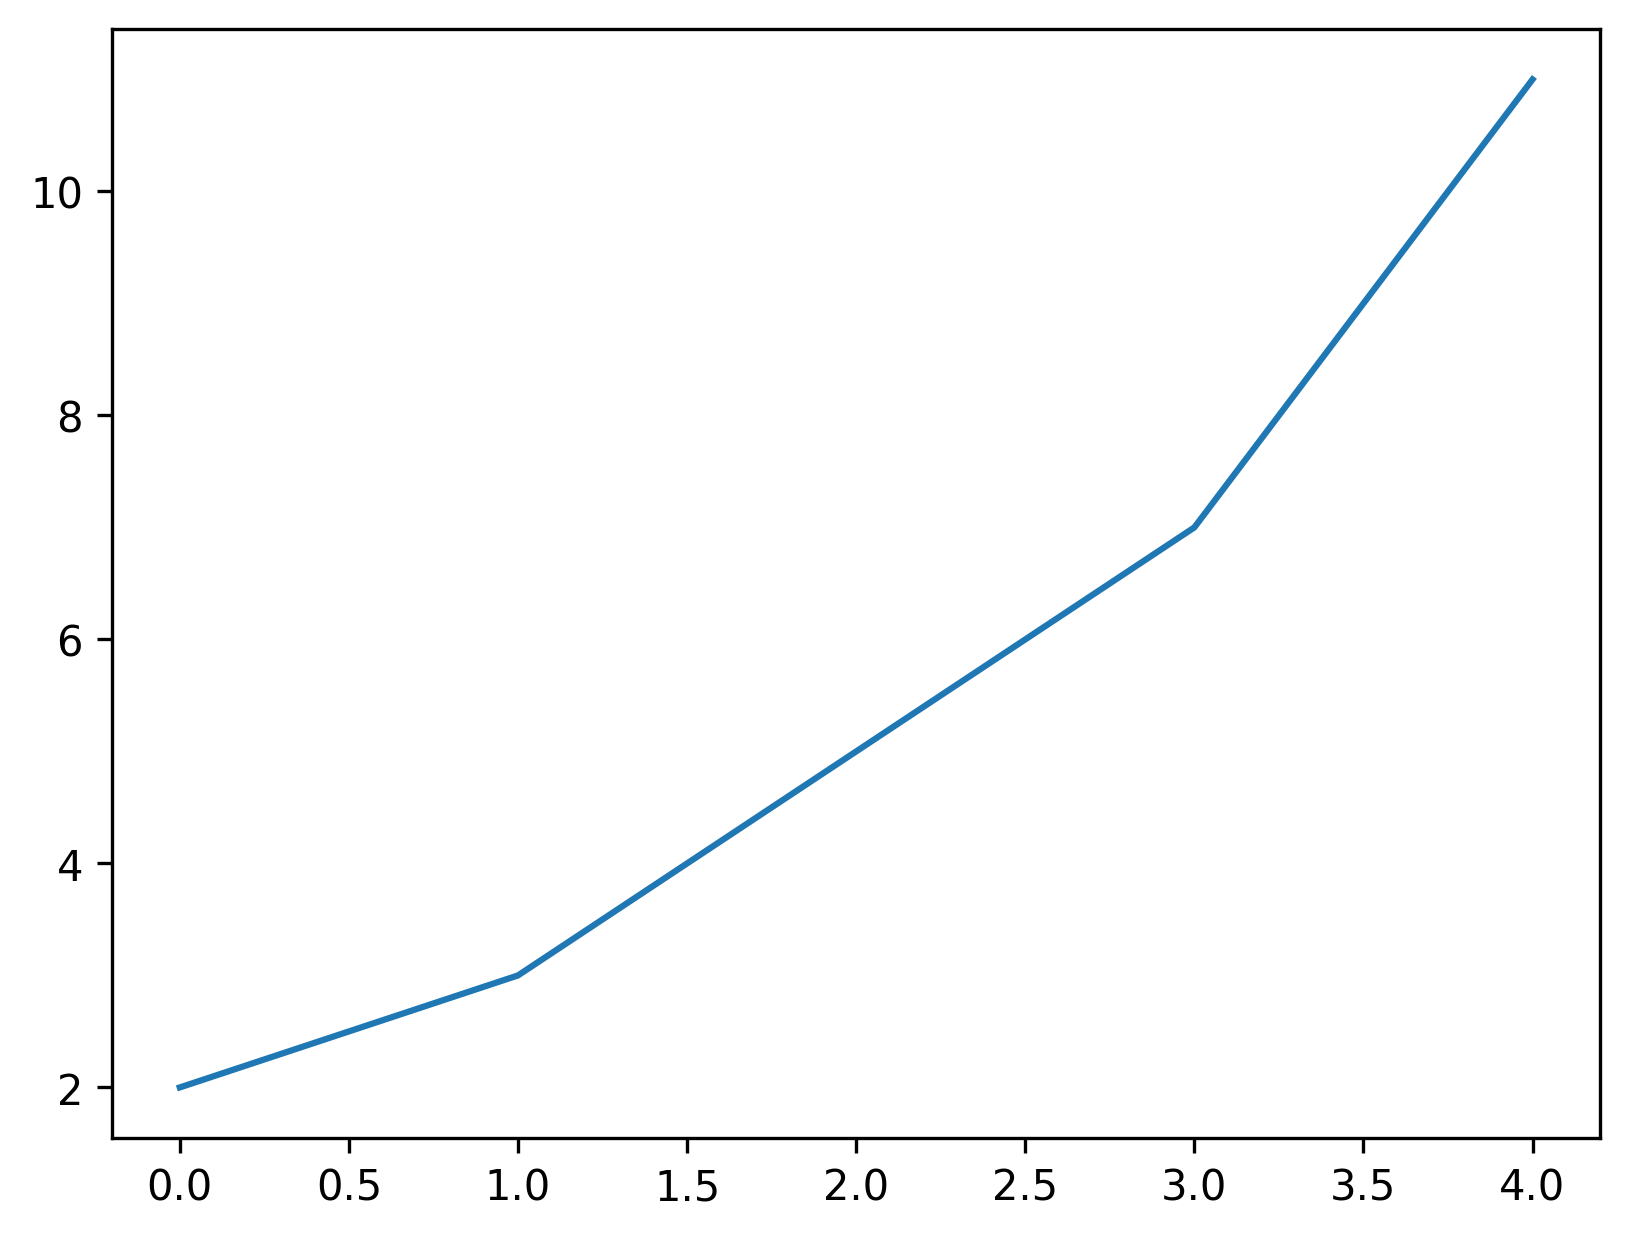
\includegraphics[width=\textwidth]{img/03-tight.png}}
        \end{column}
    \end{columns}
    \small
    \vspace{15mm}
    \hspace{-1.97mm}
    The \pycode{bbox_inches='tight'} parameter creates a tight bounding
    box for the figure.
\end{frame}


% Labels
\begin{frame}[t,fragile]
    \frametitle{Labels}
    \vspace{5mm}
    \begin{columns}[T]
        \begin{column}{0.52\textwidth}
            \pyfile{examples/04-labels.py}
        \end{column}
        \begin{column}{0.48\textwidth}
            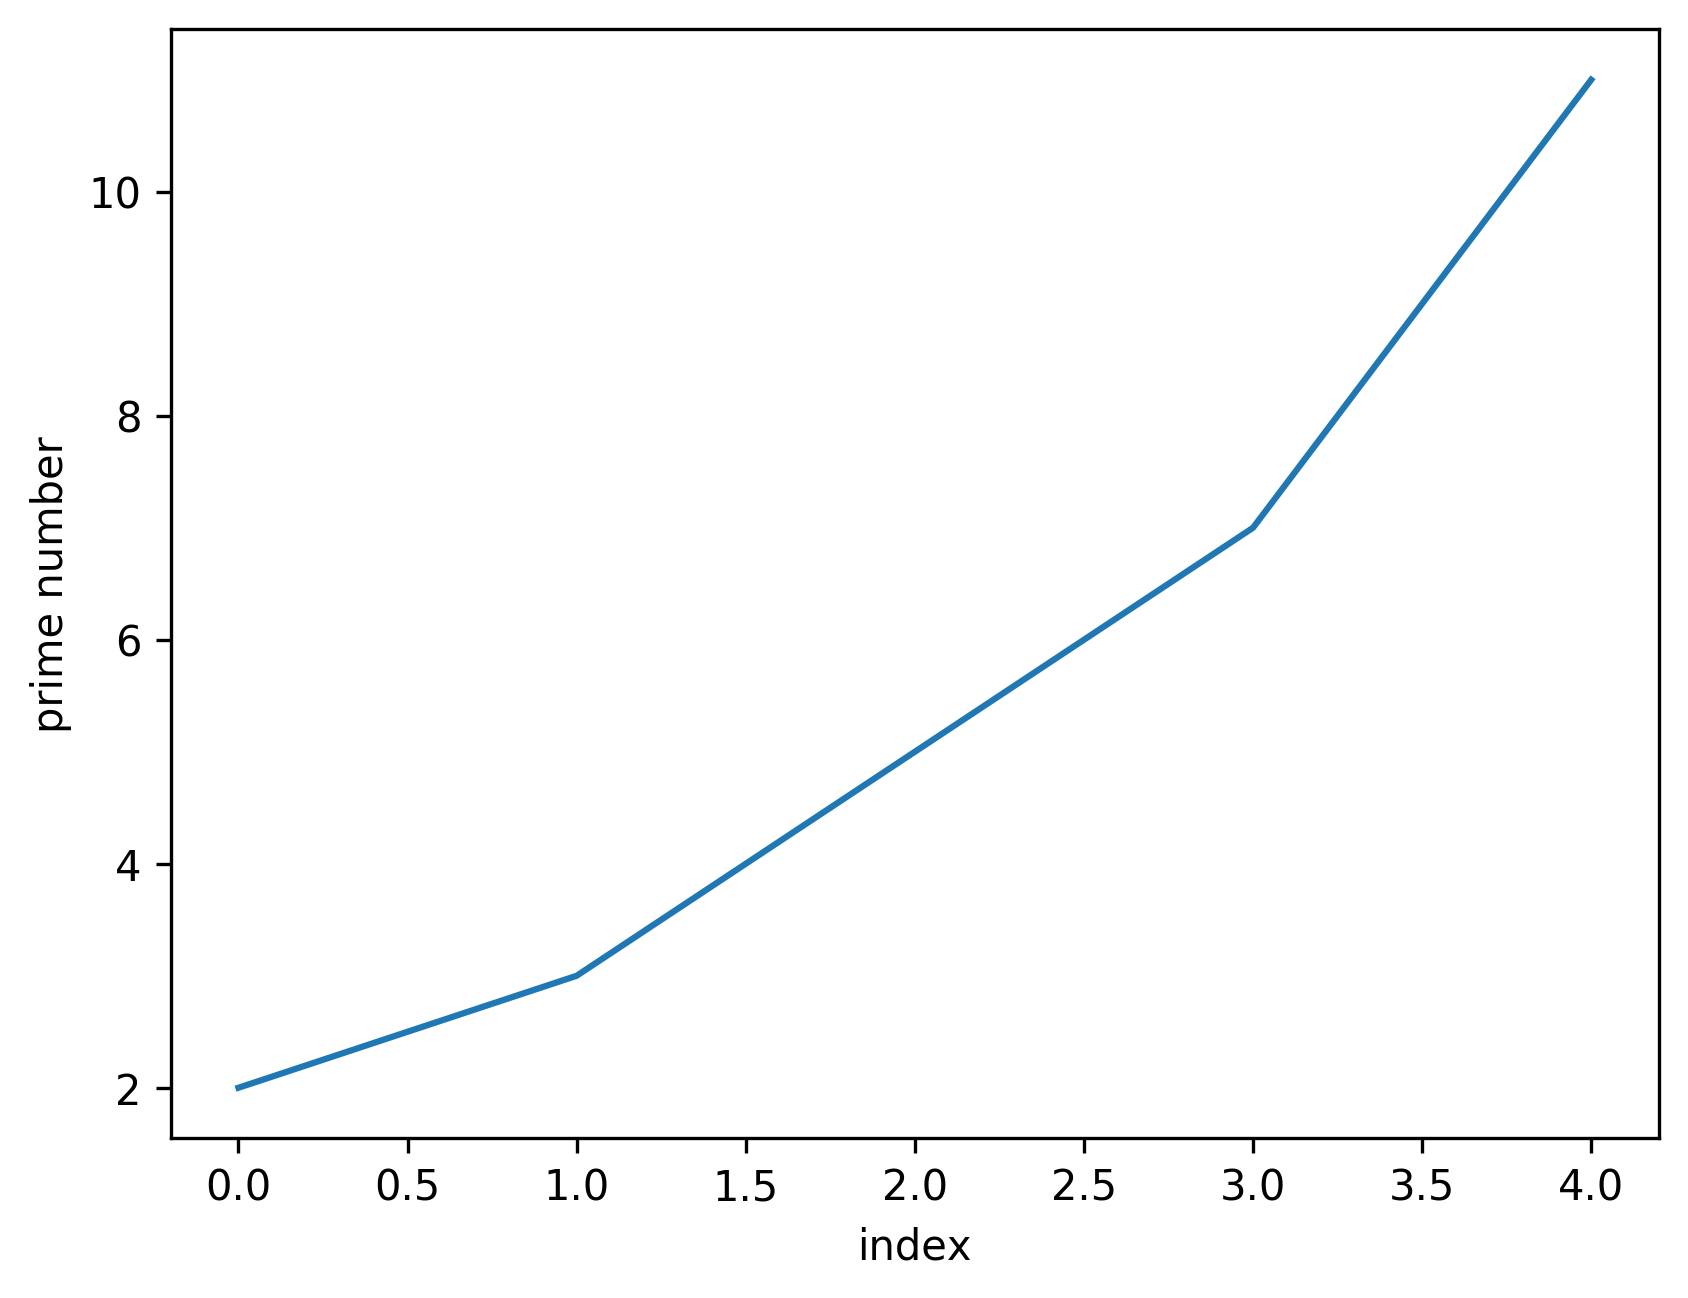
\includegraphics[width=\textwidth]{img/04-labels.png}
        \end{column}
    \end{columns}
\end{frame}


% Circle Marker and Solid Line
\begin{frame}[t,fragile]
    \frametitle{Circle Marker and Solid Line}
    \vspace{5mm}
    \begin{columns}[T]
        \begin{column}{0.52\textwidth}
            \pyfile{examples/05-circle-marker-solid.py}
        \end{column}
        \begin{column}{0.48\textwidth}
            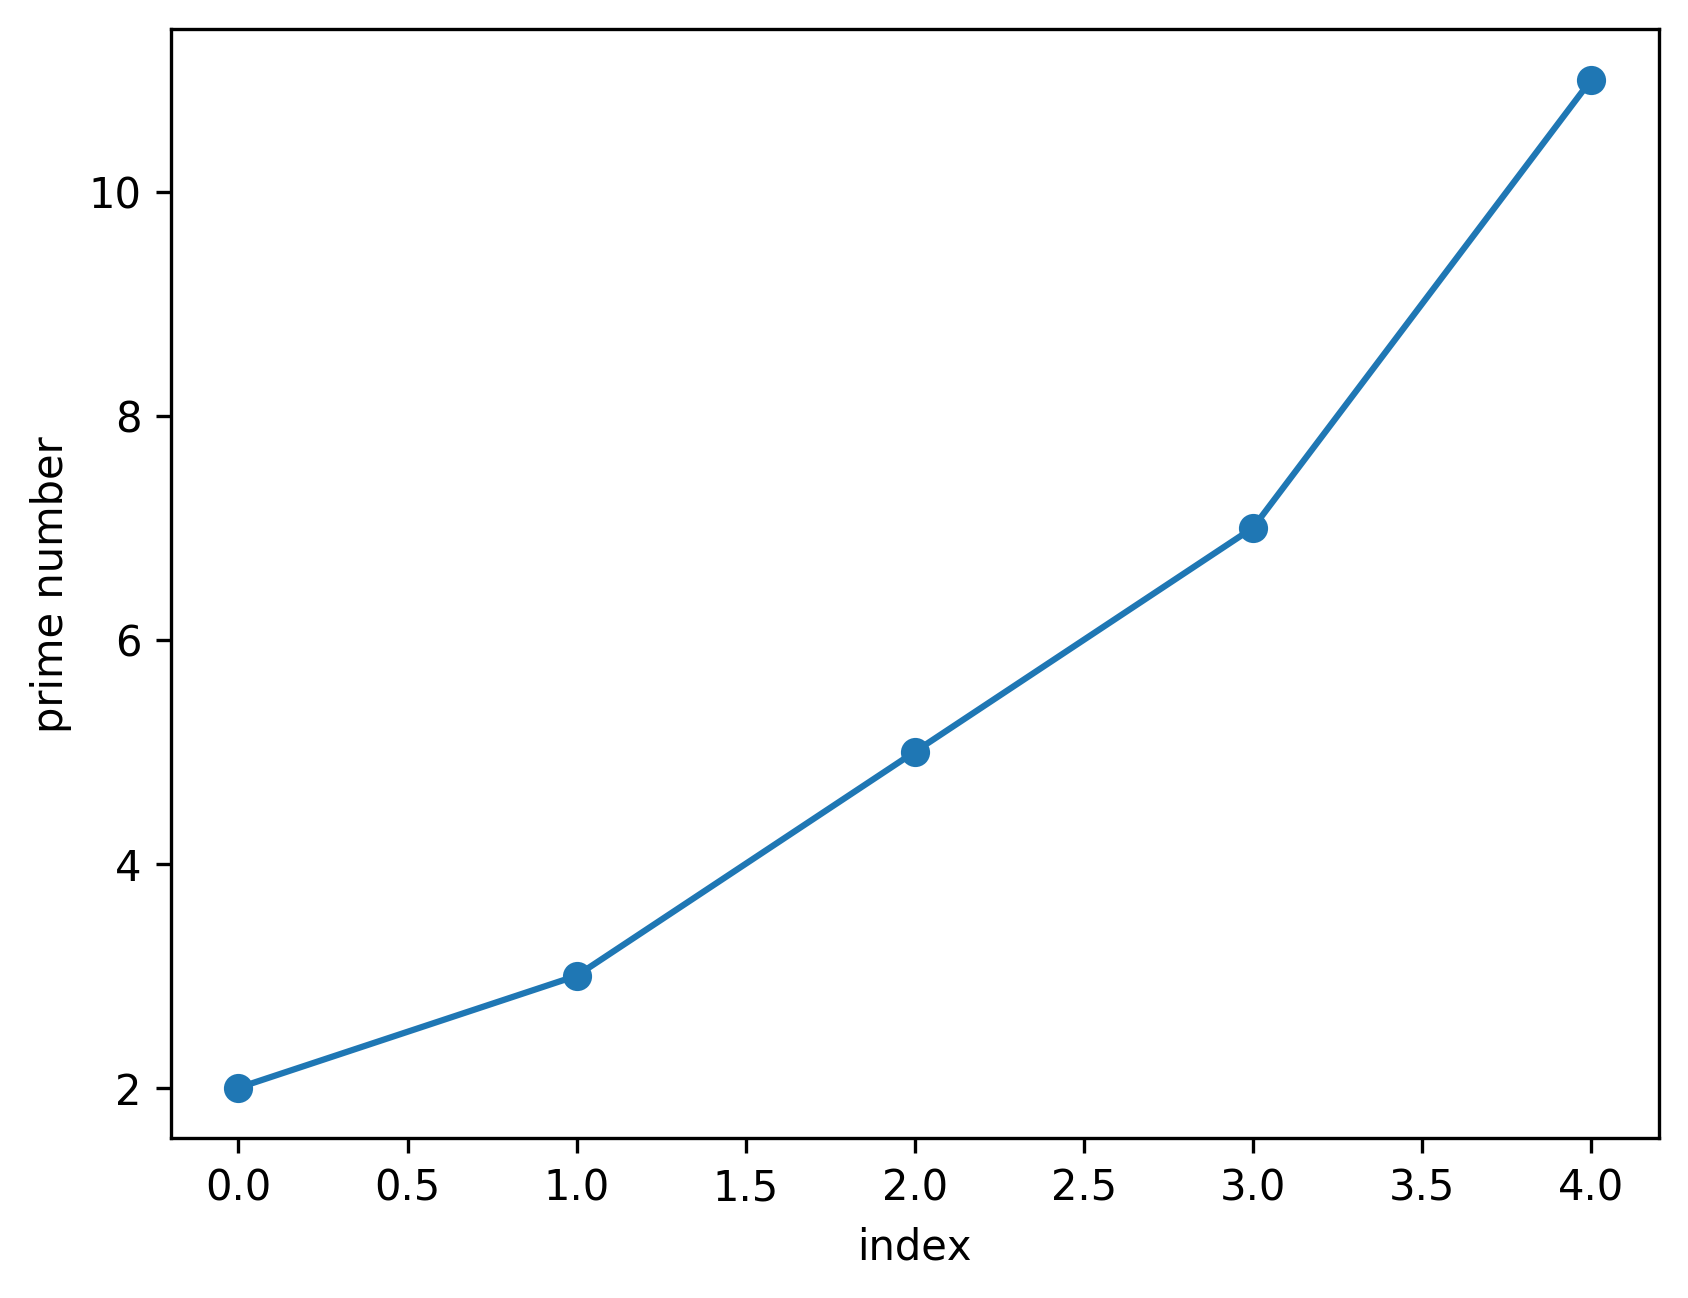
\includegraphics[width=\textwidth]{img/05-circle-marker-solid.png}
        \end{column}
    \end{columns}
\end{frame}


% Integer Ticks
\begin{frame}[t,fragile]
    \frametitle{Integer Ticks}
    \vspace{5mm}
    \begin{columns}[T]
        \begin{column}{0.52\textwidth}
            \pyfile{examples/06-ticks.py}
        \end{column}
        \begin{column}{0.48\textwidth}
            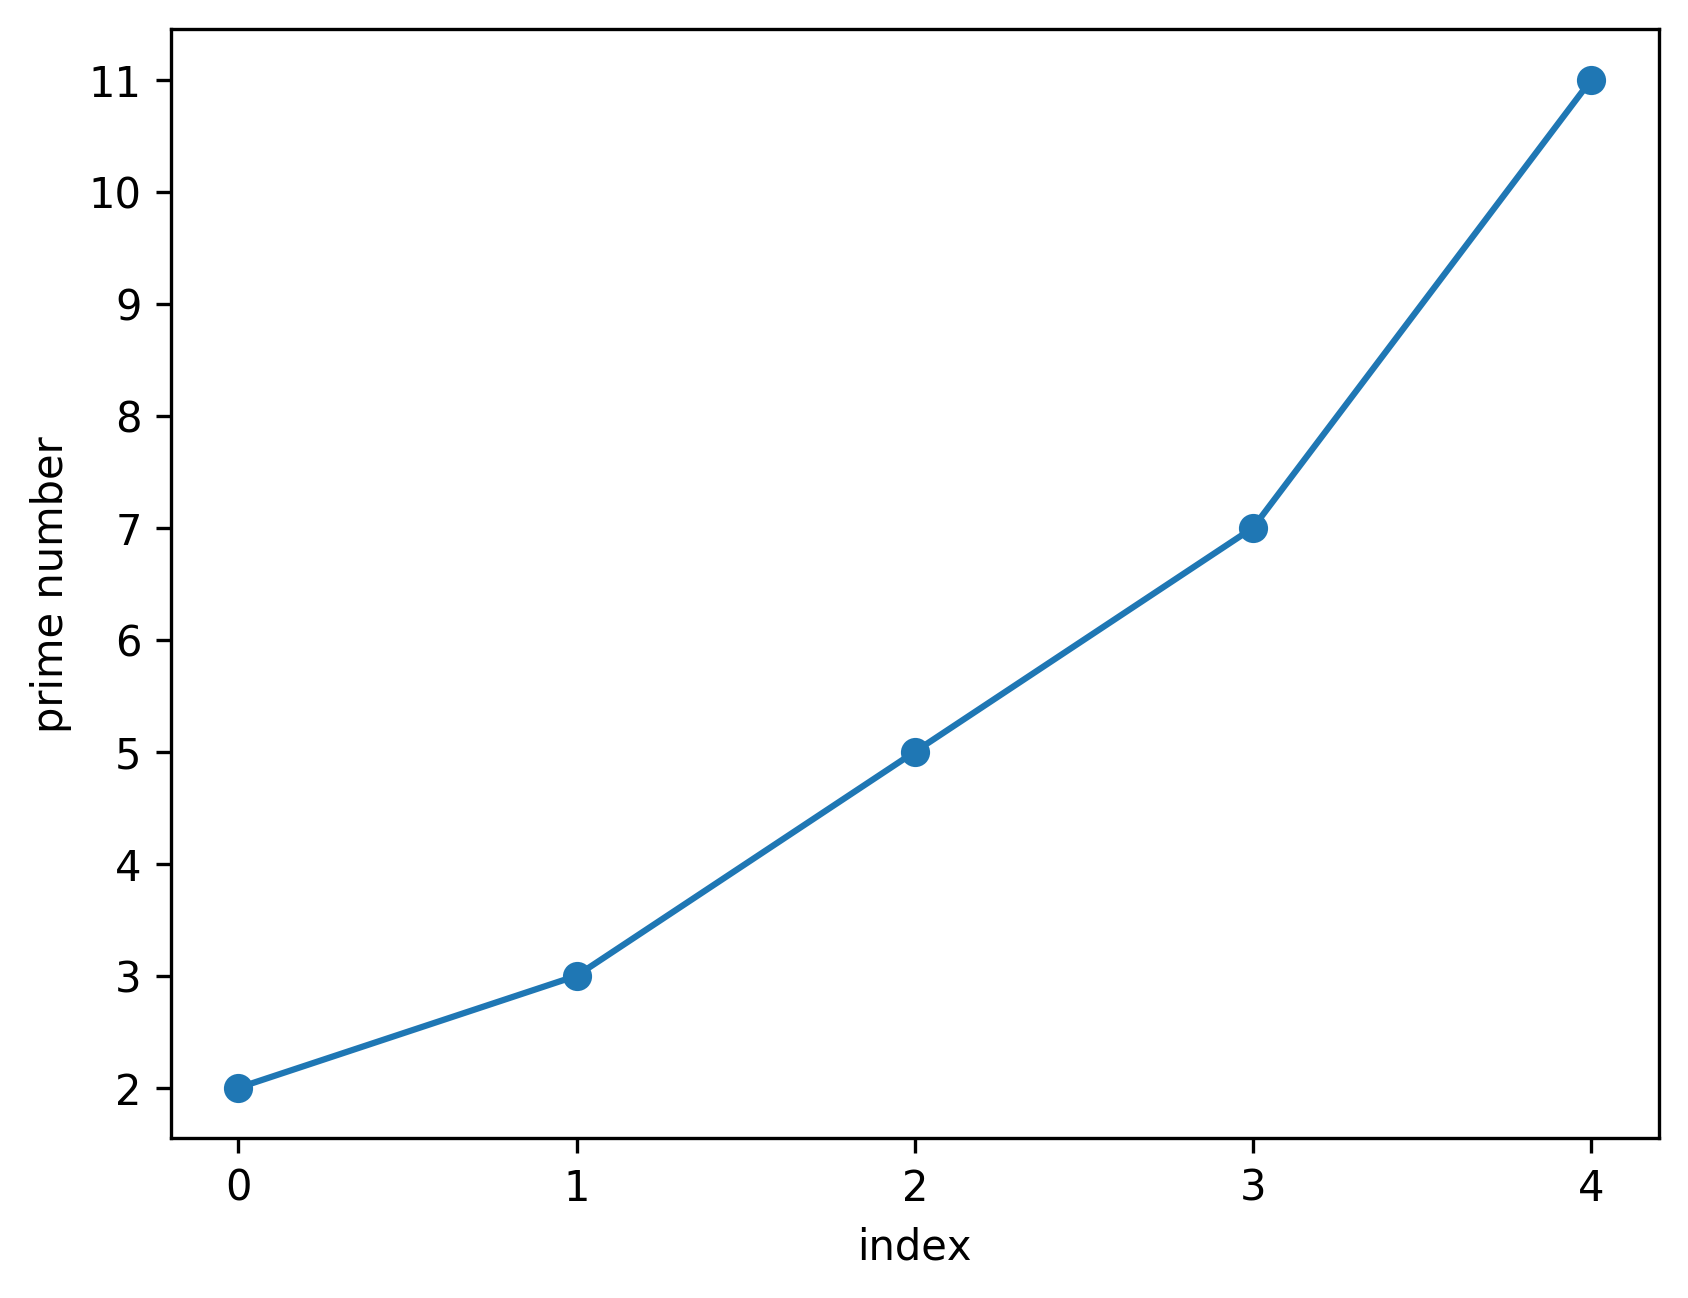
\includegraphics[width=\textwidth]{img/06-ticks.png}
        \end{column}
    \end{columns}
\end{frame}


% Format String
\begin{frame}[t,fragile]
    \frametitle{Format String}

    \textbf{Syntax:}

    \pycode{[marker][line][color]}

    \medskip
    \pause

    \textbf{Example:}

    \pycode{'o-k'}

    \medskip
    \pause

    \textbf{Explanation:}
    \begin{itemize}
        \item \pycode{'o'} for circle marker
        \item \pycode{'-'} for solid line style
        \item \pycode{'k'} for black color
    \end{itemize}

    \medskip
    \pause

    \textbf{Usage:}

    \begin{pyenv}[gobble=8]
        plt.plot([2, 3, 5, 7, 11], 'o-k')
    \end{pyenv}

\end{frame}


% Point Marker
\begin{frame}[t,fragile]
    \frametitle{Point Marker}
    \vspace{5mm}
    \begin{columns}[T]
        \begin{column}{0.52\textwidth}
            \pyfile{examples/07-point-marker.py}
        \end{column}
        \begin{column}{0.48\textwidth}
            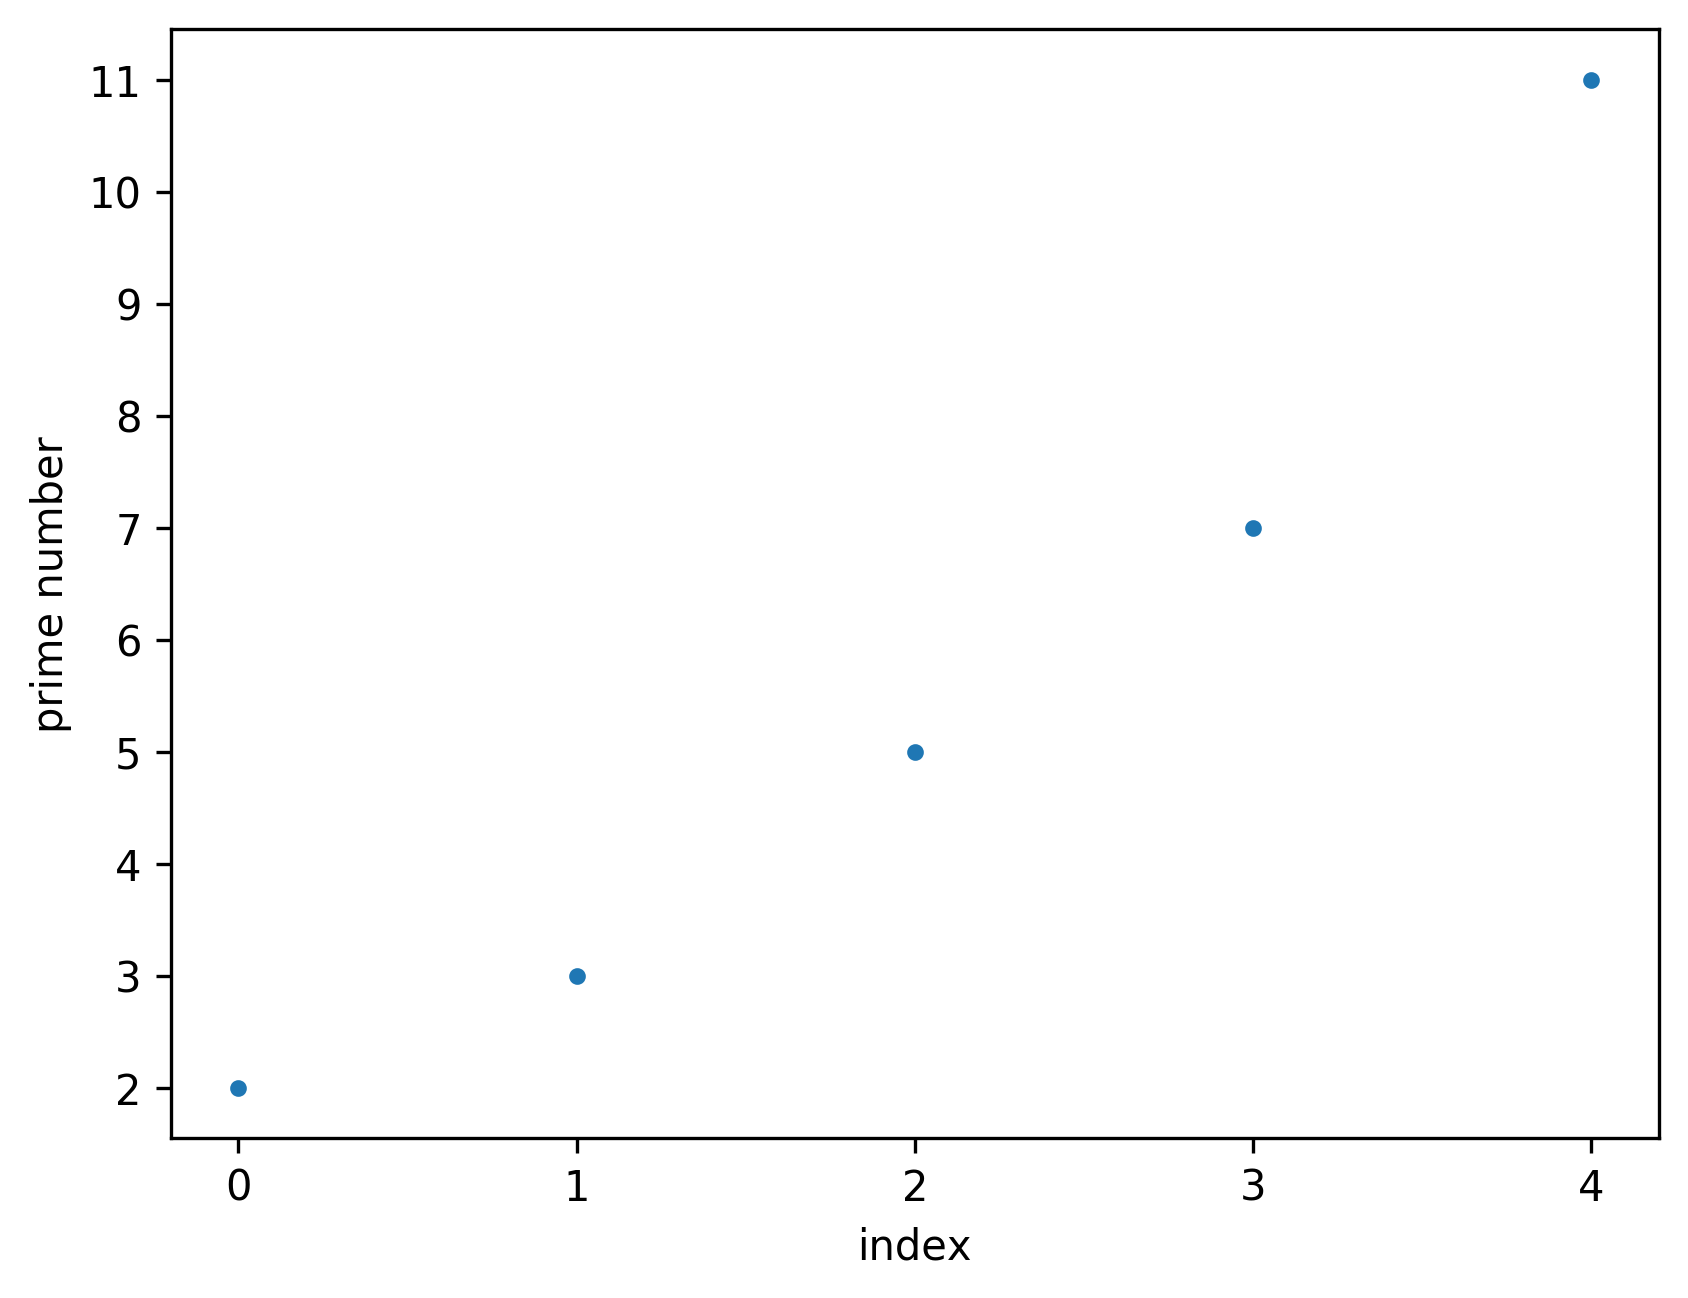
\includegraphics[width=\textwidth]{img/07-point-marker.png}
        \end{column}
    \end{columns}
\end{frame}


% Circle Marker
\begin{frame}[t,fragile]
    \frametitle{Circle Marker}
    \vspace{5mm}
    \begin{columns}[T]
        \begin{column}{0.52\textwidth}
            \pyfile{examples/08-circle-marker.py}
        \end{column}
        \begin{column}{0.48\textwidth}
            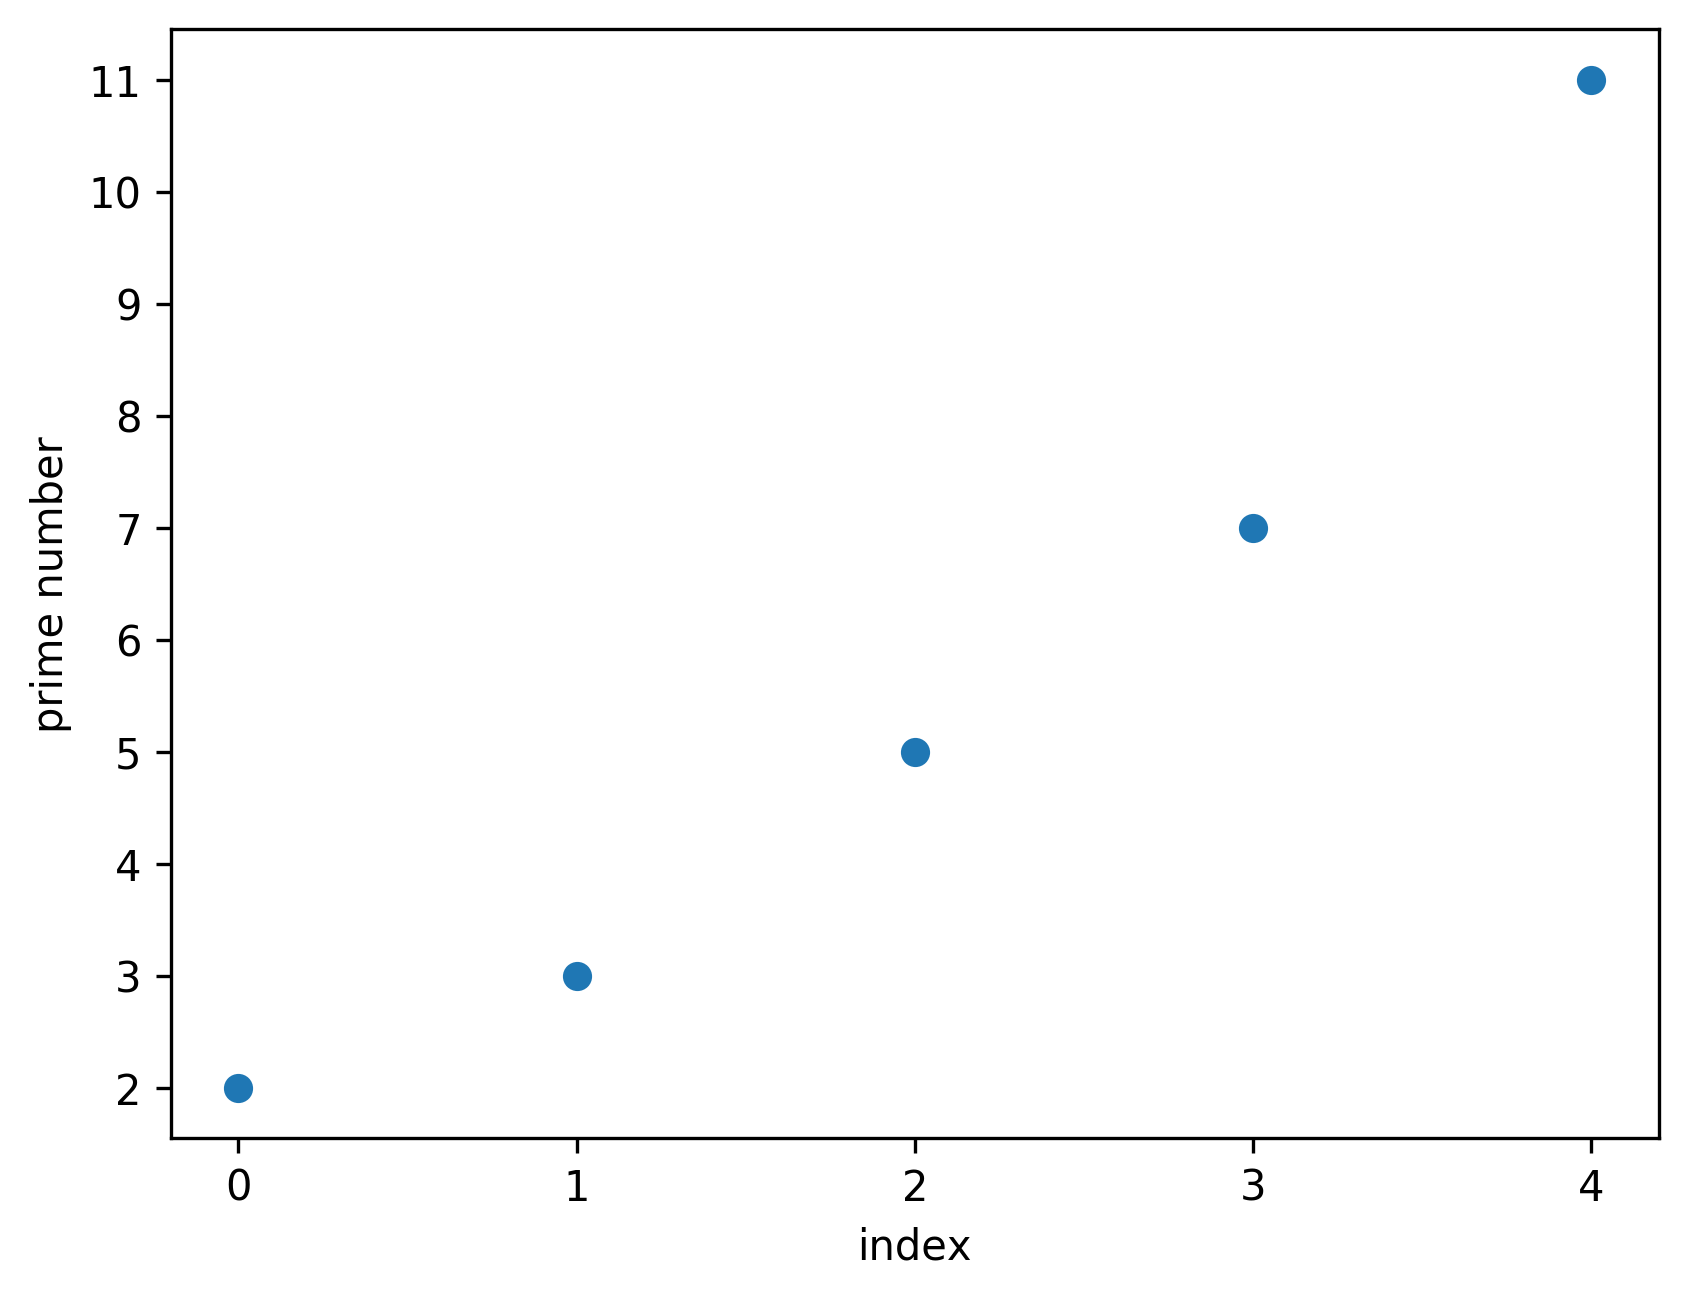
\includegraphics[width=\textwidth]{img/08-circle-marker.png}
        \end{column}
    \end{columns}
\end{frame}


% Triangle Down Marker
\begin{frame}[t,fragile]
    \frametitle{Triangle Down Marker}
    \vspace{5mm}
    \begin{columns}[T]
        \begin{column}{0.52\textwidth}
            \pyfile{examples/09-triangle-marker.py}
        \end{column}
        \begin{column}{0.48\textwidth}
            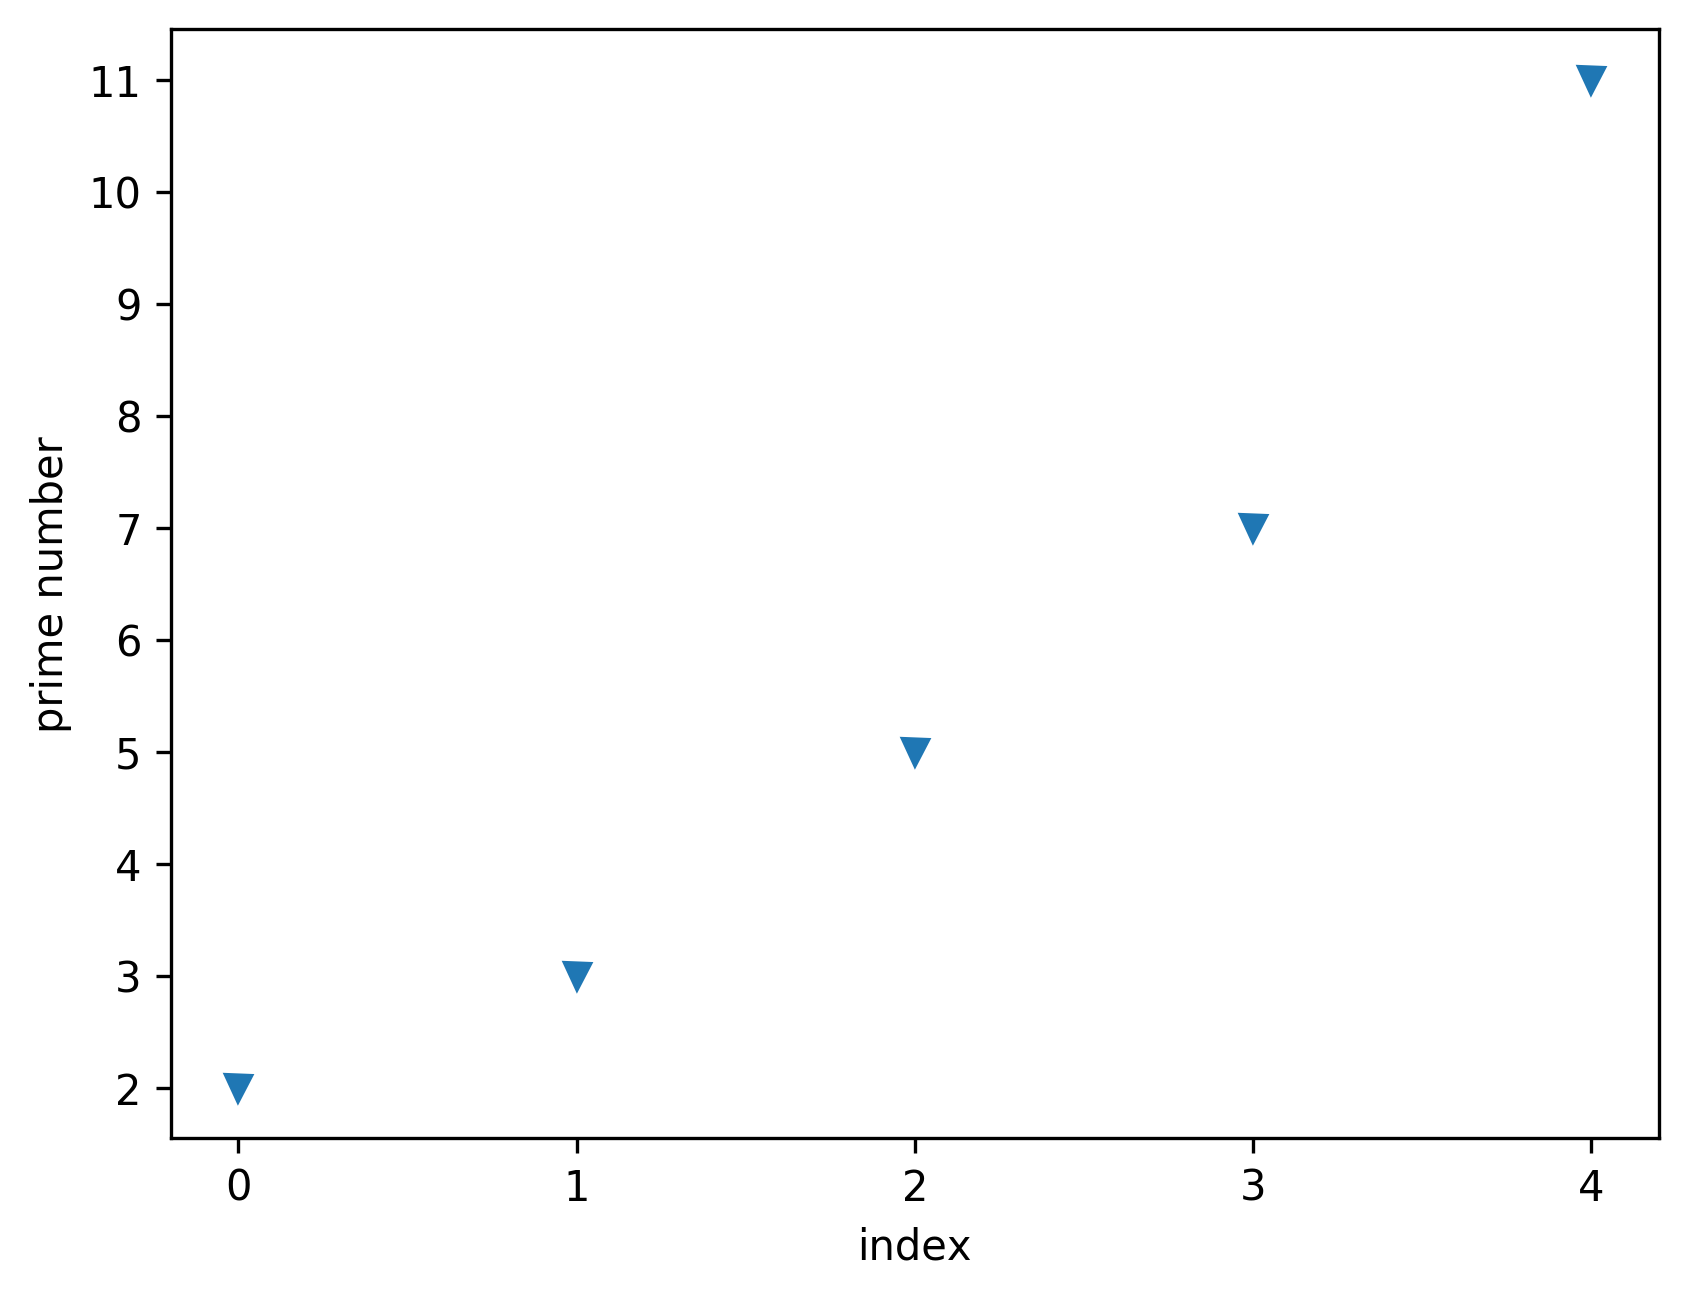
\includegraphics[width=\textwidth]{img/09-triangle-marker.png}
        \end{column}
    \end{columns}
\end{frame}


% Square Marker
\begin{frame}[t,fragile]
    \frametitle{Square Marker}
    \vspace{5mm}
    \begin{columns}[T]
        \begin{column}{0.52\textwidth}
            \pyfile{examples/10-square-marker.py}
        \end{column}
        \begin{column}{0.48\textwidth}
            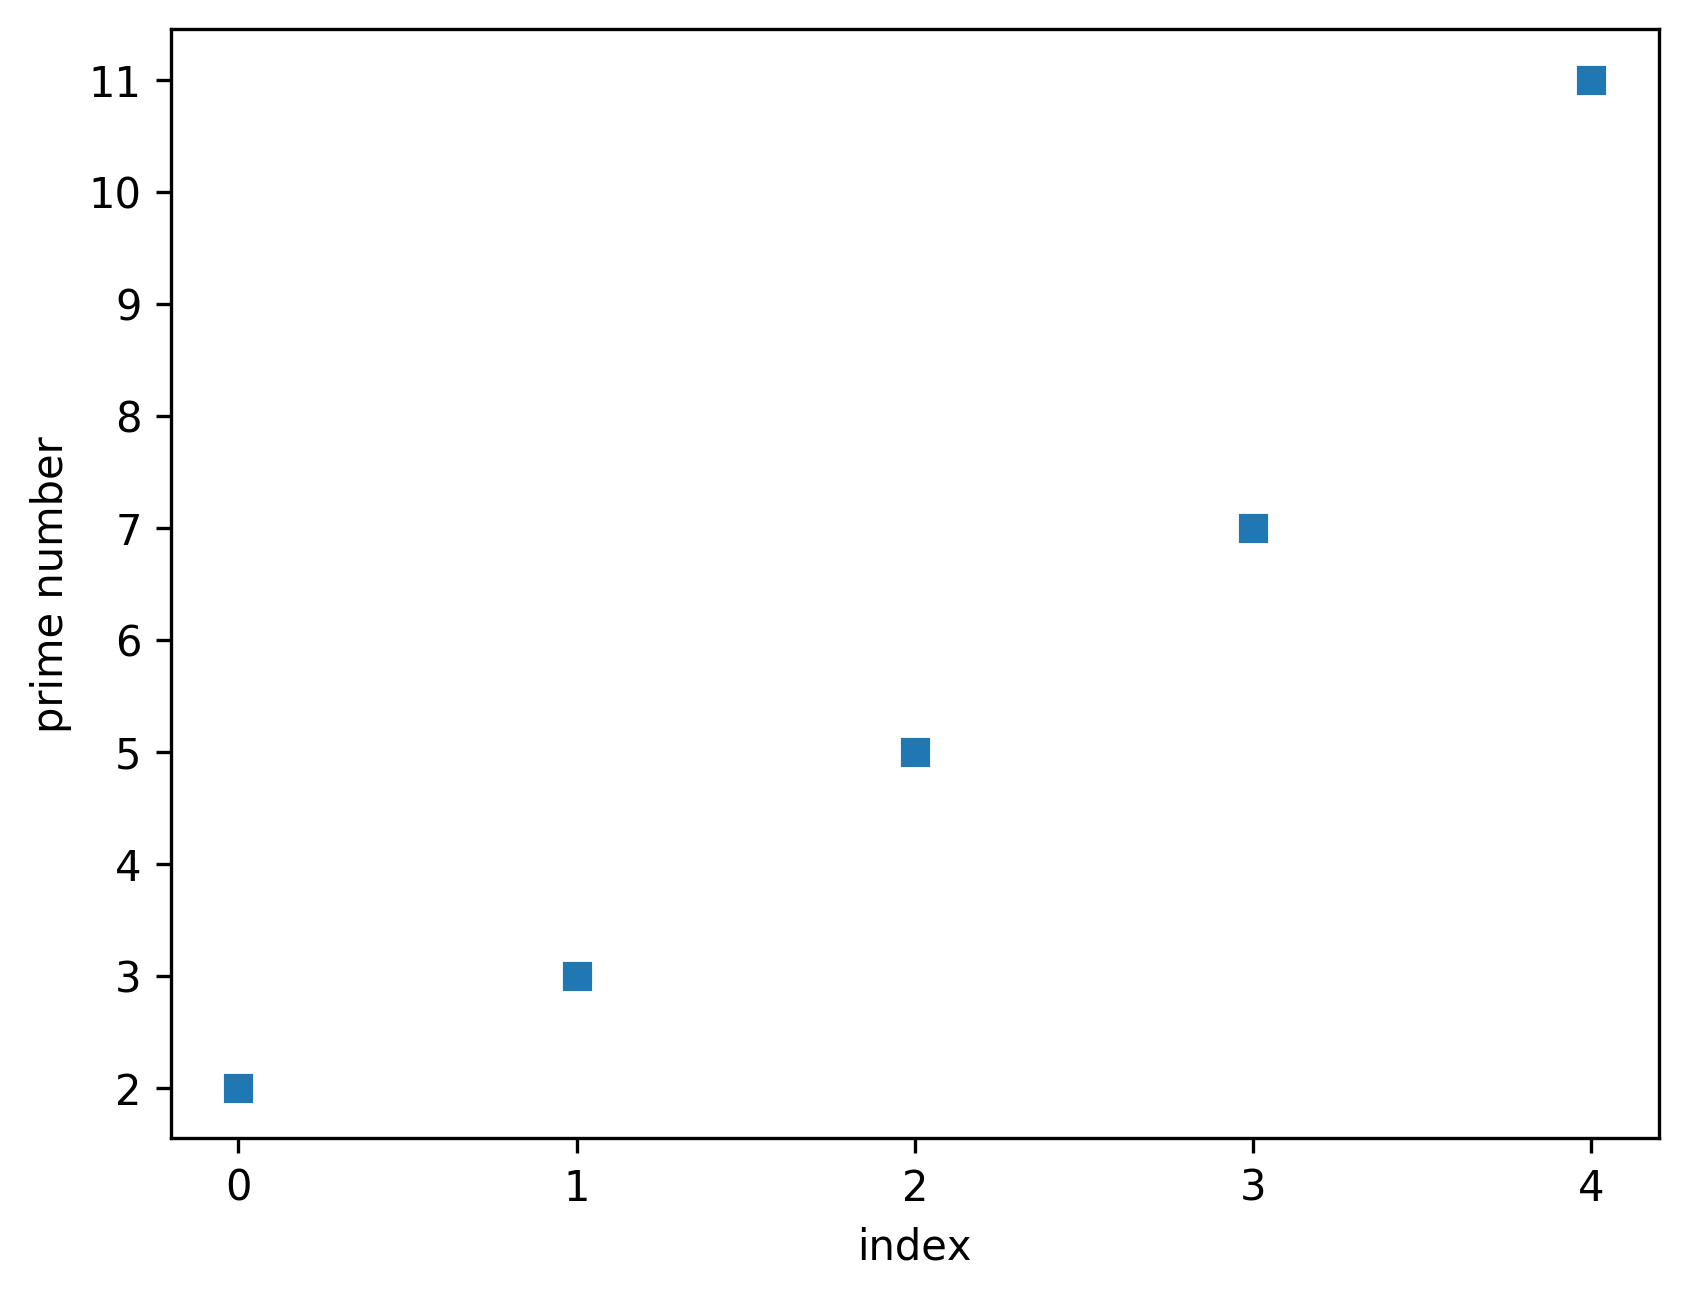
\includegraphics[width=\textwidth]{img/10-square-marker.png}
        \end{column}
    \end{columns}
\end{frame}


% Markers Reference
\begin{frame}[t,fragile]
    \frametitle{Markers Reference}
    \begin{columns}[T]
        \begin{column}{0.45\textwidth}
            \vspace{-1.5mm}
            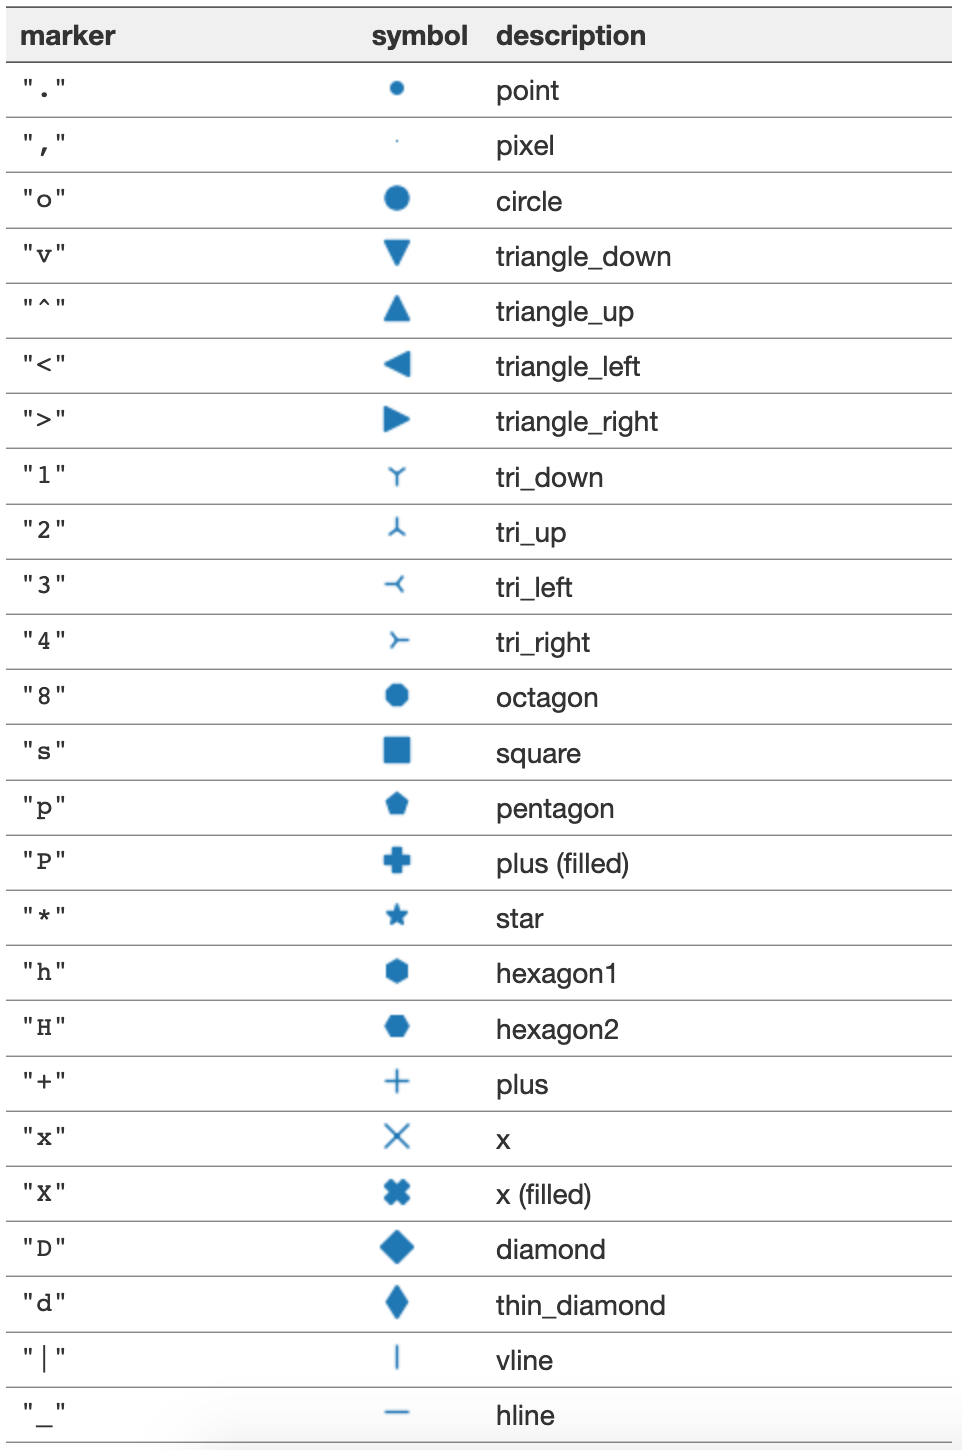
\includegraphics[height=75mm]{img/ref-markers.png}
        \end{column}
        \begin{column}{0.55\textwidth}
            \vspace{33mm}
            \footnotesize
            Source:\\
            \url{https://matplotlib.org/api/markers_api.html}
        \end{column}
    \end{columns}
\end{frame}


% Solid Line Style
\begin{frame}[t,fragile]
    \frametitle{Solid Line Style}
    \vspace{5mm}
    \begin{columns}[T]
        \begin{column}{0.52\textwidth}
            \pyfile{examples/11-solid-line-style.py}
        \end{column}
        \begin{column}{0.48\textwidth}
            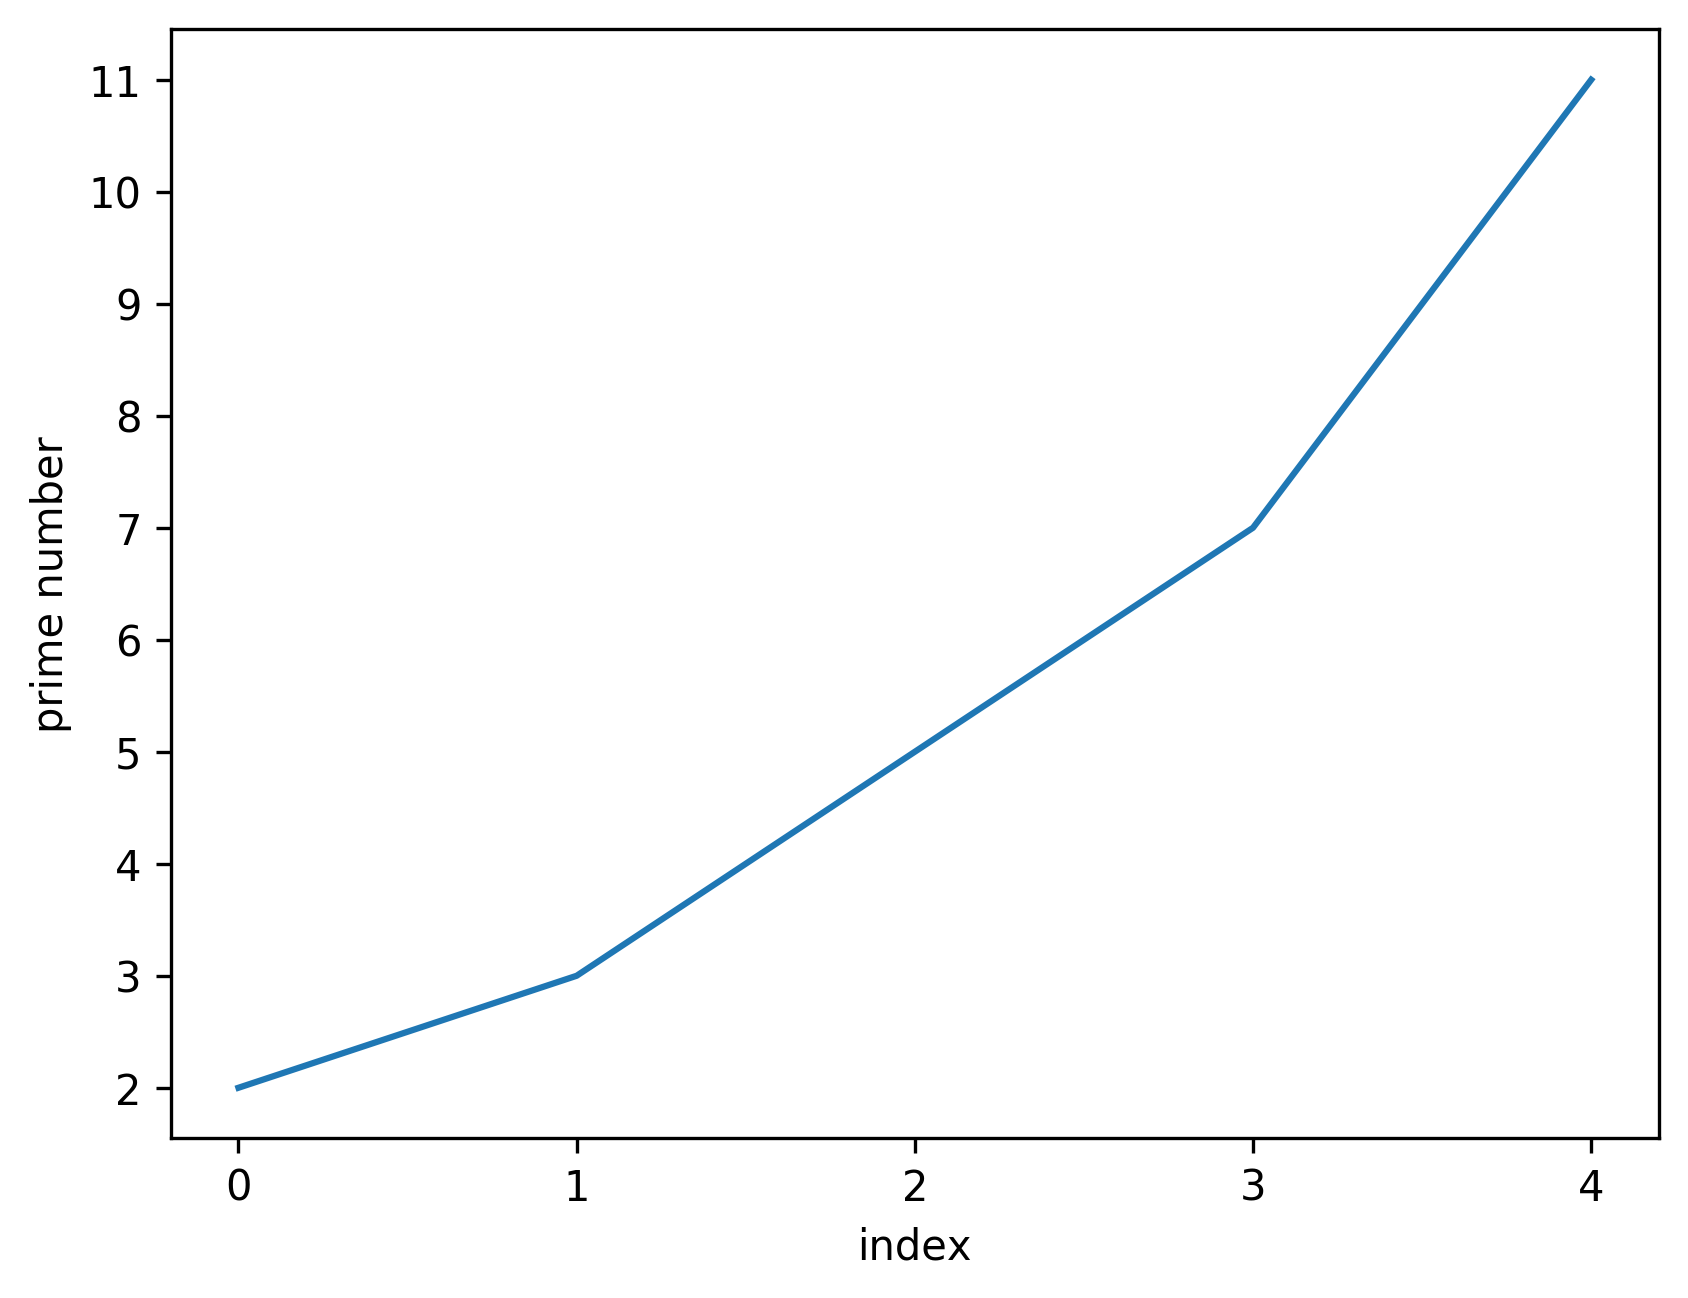
\includegraphics[width=\textwidth]{img/11-solid-line-style.png}
        \end{column}
    \end{columns}
\end{frame}


% Dashed Line Style
\begin{frame}[t,fragile]
    \frametitle{Dashed Line Style}
    \vspace{5mm}
    \begin{columns}[T]
        \begin{column}{0.52\textwidth}
            \pyfile{examples/12-dashed-line-style.py}
        \end{column}
        \begin{column}{0.48\textwidth}
            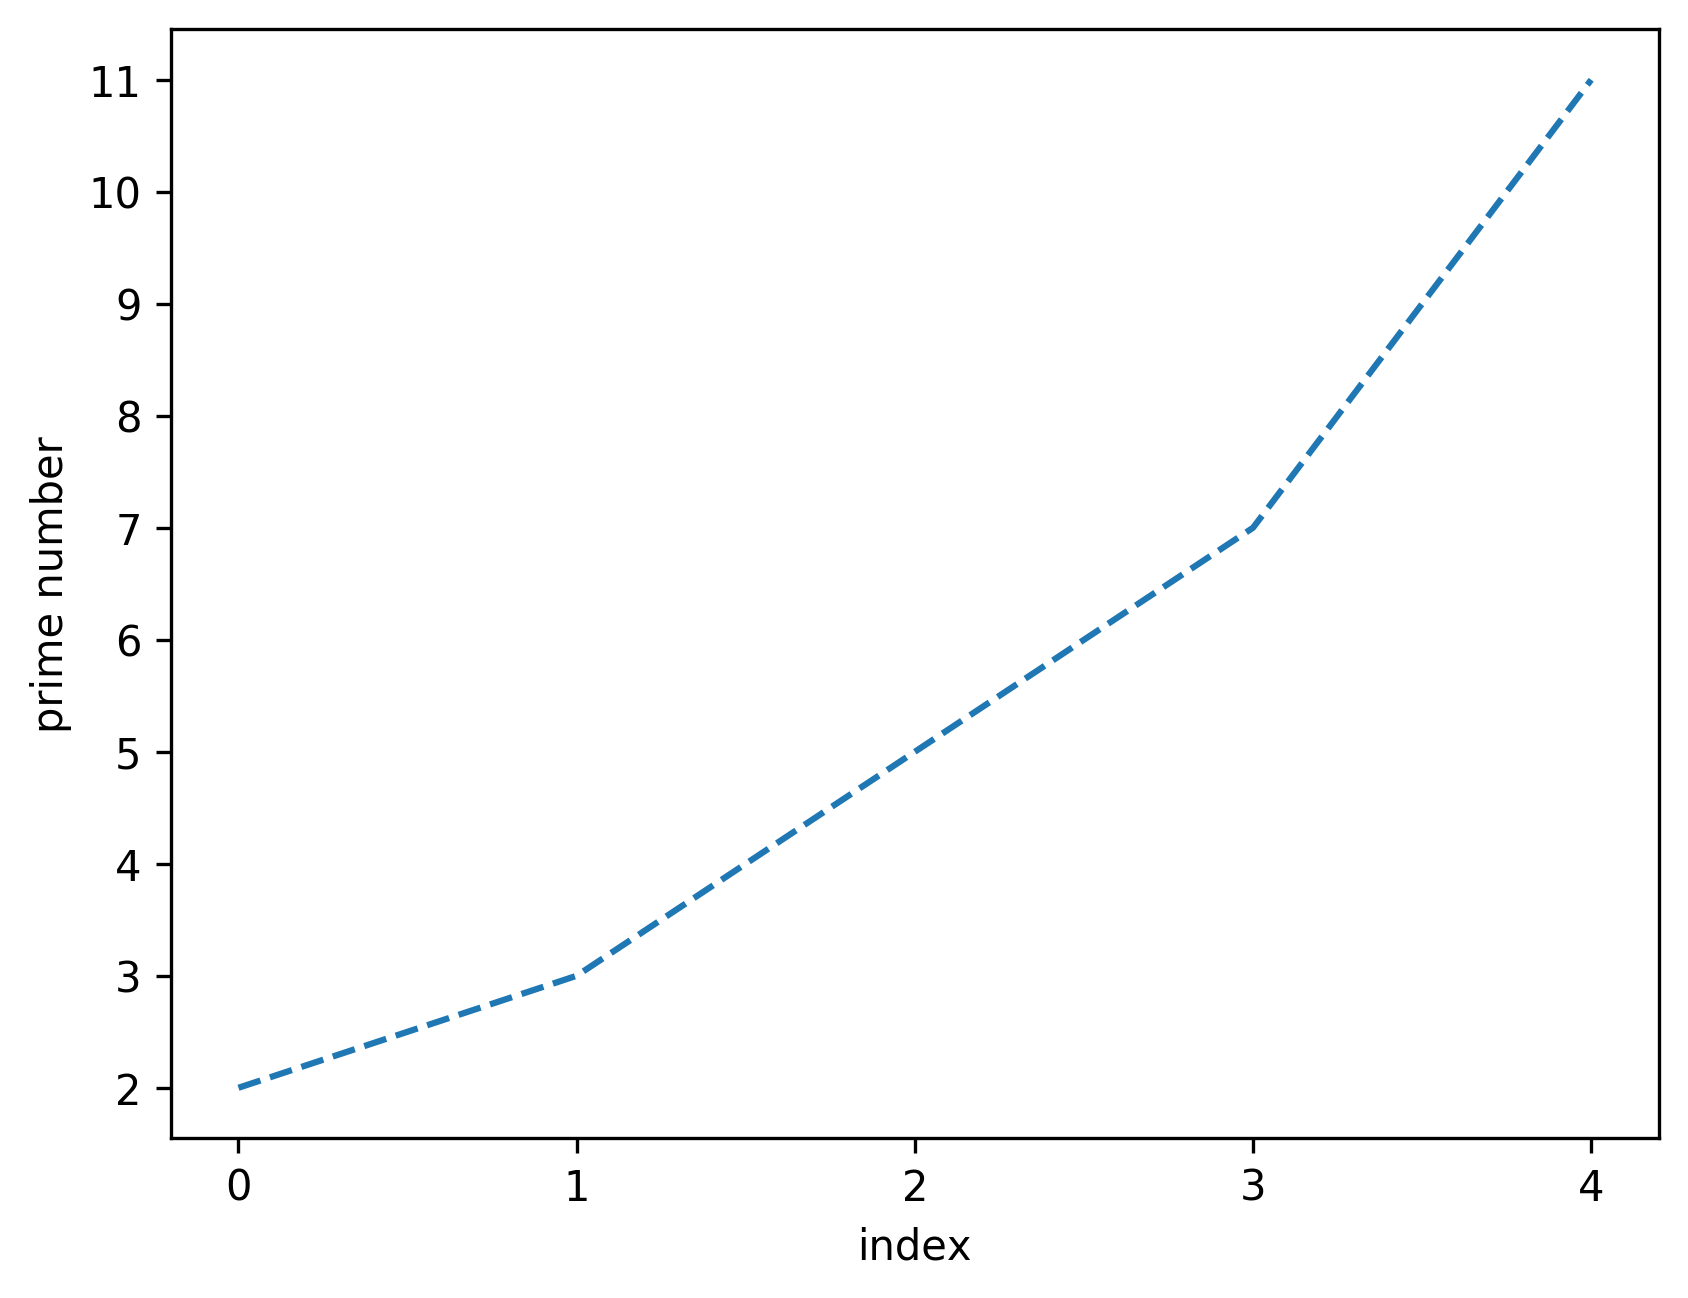
\includegraphics[width=\textwidth]{img/12-dashed-line-style.png}
        \end{column}
    \end{columns}
\end{frame}


% Dash-Dot Line Style
\begin{frame}[t,fragile]
    \frametitle{Dash-Dot Line Style}
    \vspace{5mm}
    \begin{columns}[T]
        \begin{column}{0.52\textwidth}
            \pyfile{examples/13-dash-dot-line-style.py}
        \end{column}
        \begin{column}{0.48\textwidth}
            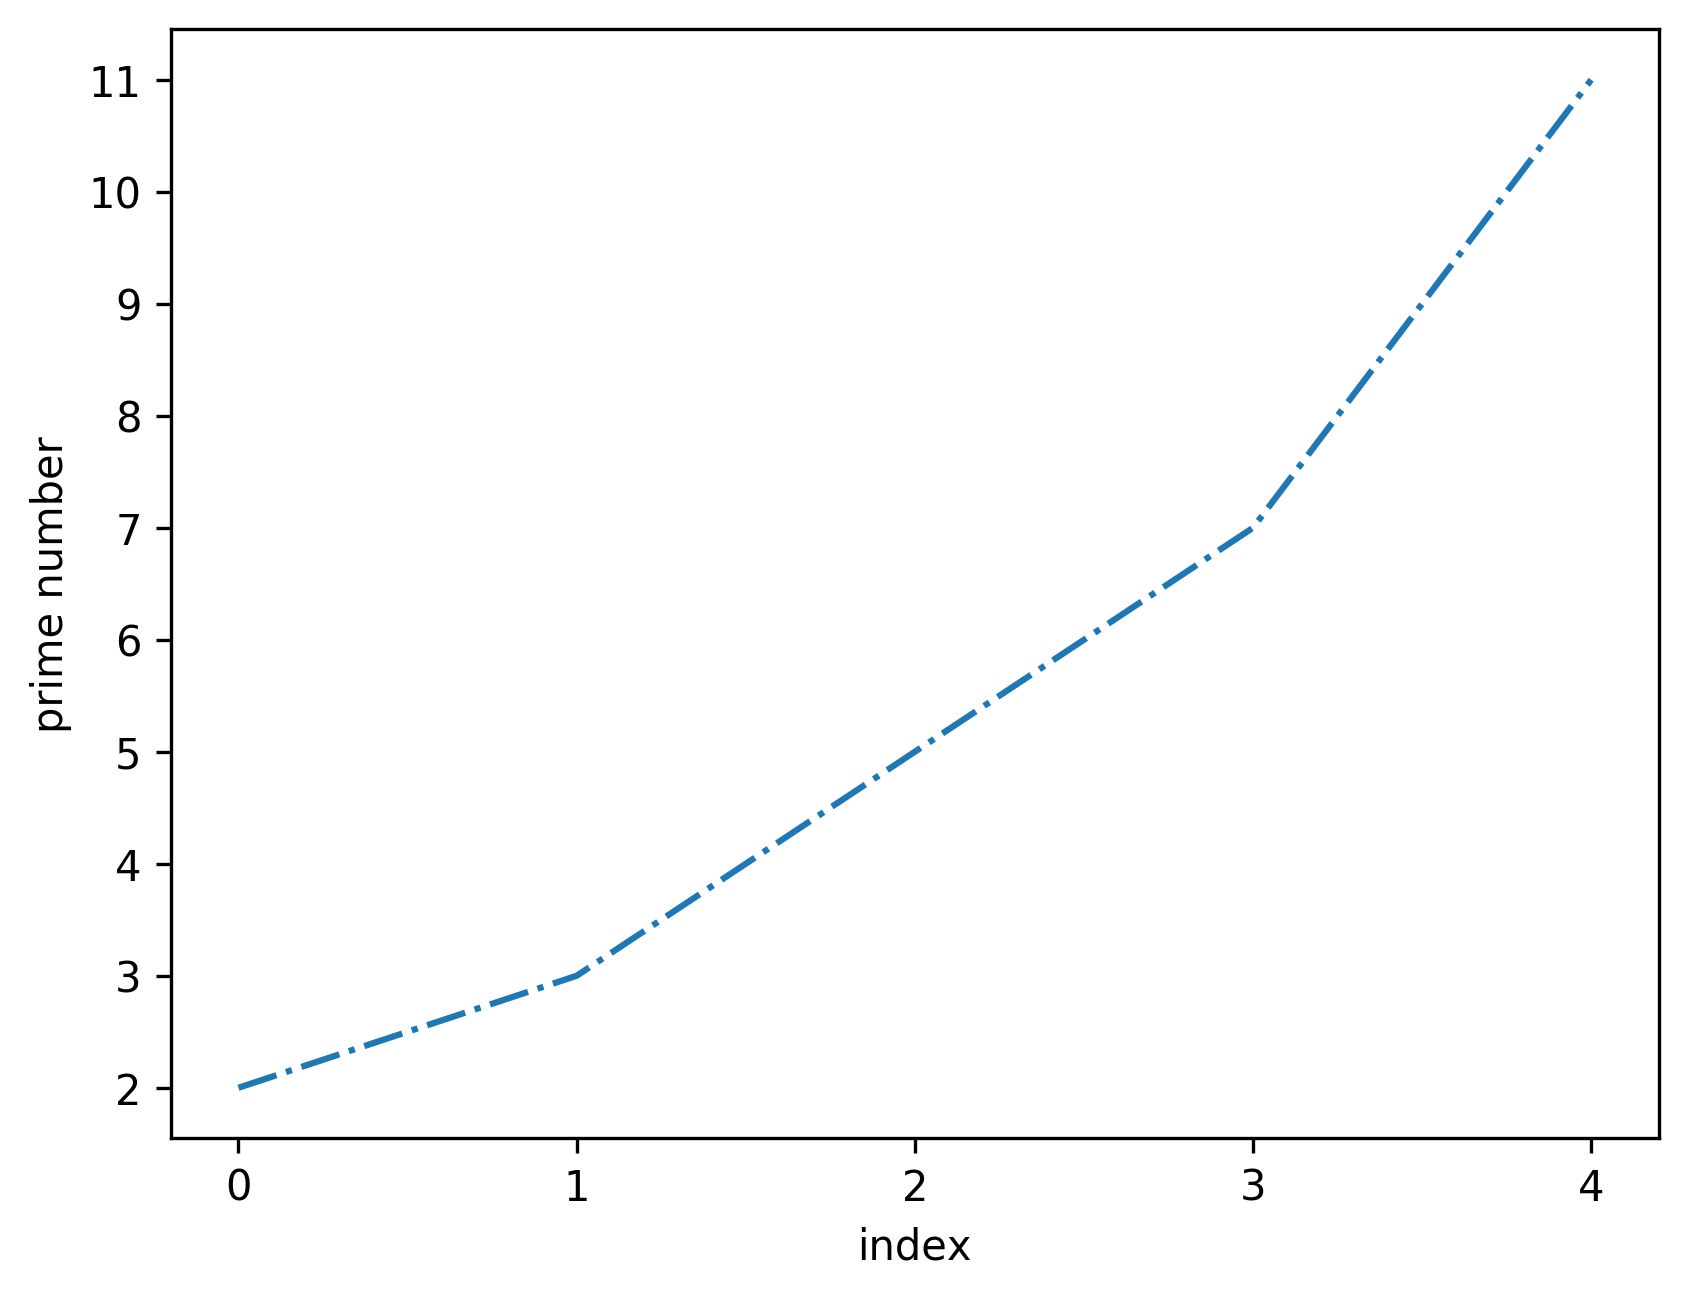
\includegraphics[width=\textwidth]{img/13-dash-dot-line-style.png}
        \end{column}
    \end{columns}
\end{frame}


% Dotted Line Style
\begin{frame}[t,fragile]
    \frametitle{Dotted Line Style}
    \vspace{5mm}
    \begin{columns}[T]
        \begin{column}{0.52\textwidth}
            \pyfile{examples/14-dotted-line-style.py}
        \end{column}
        \begin{column}{0.48\textwidth}
            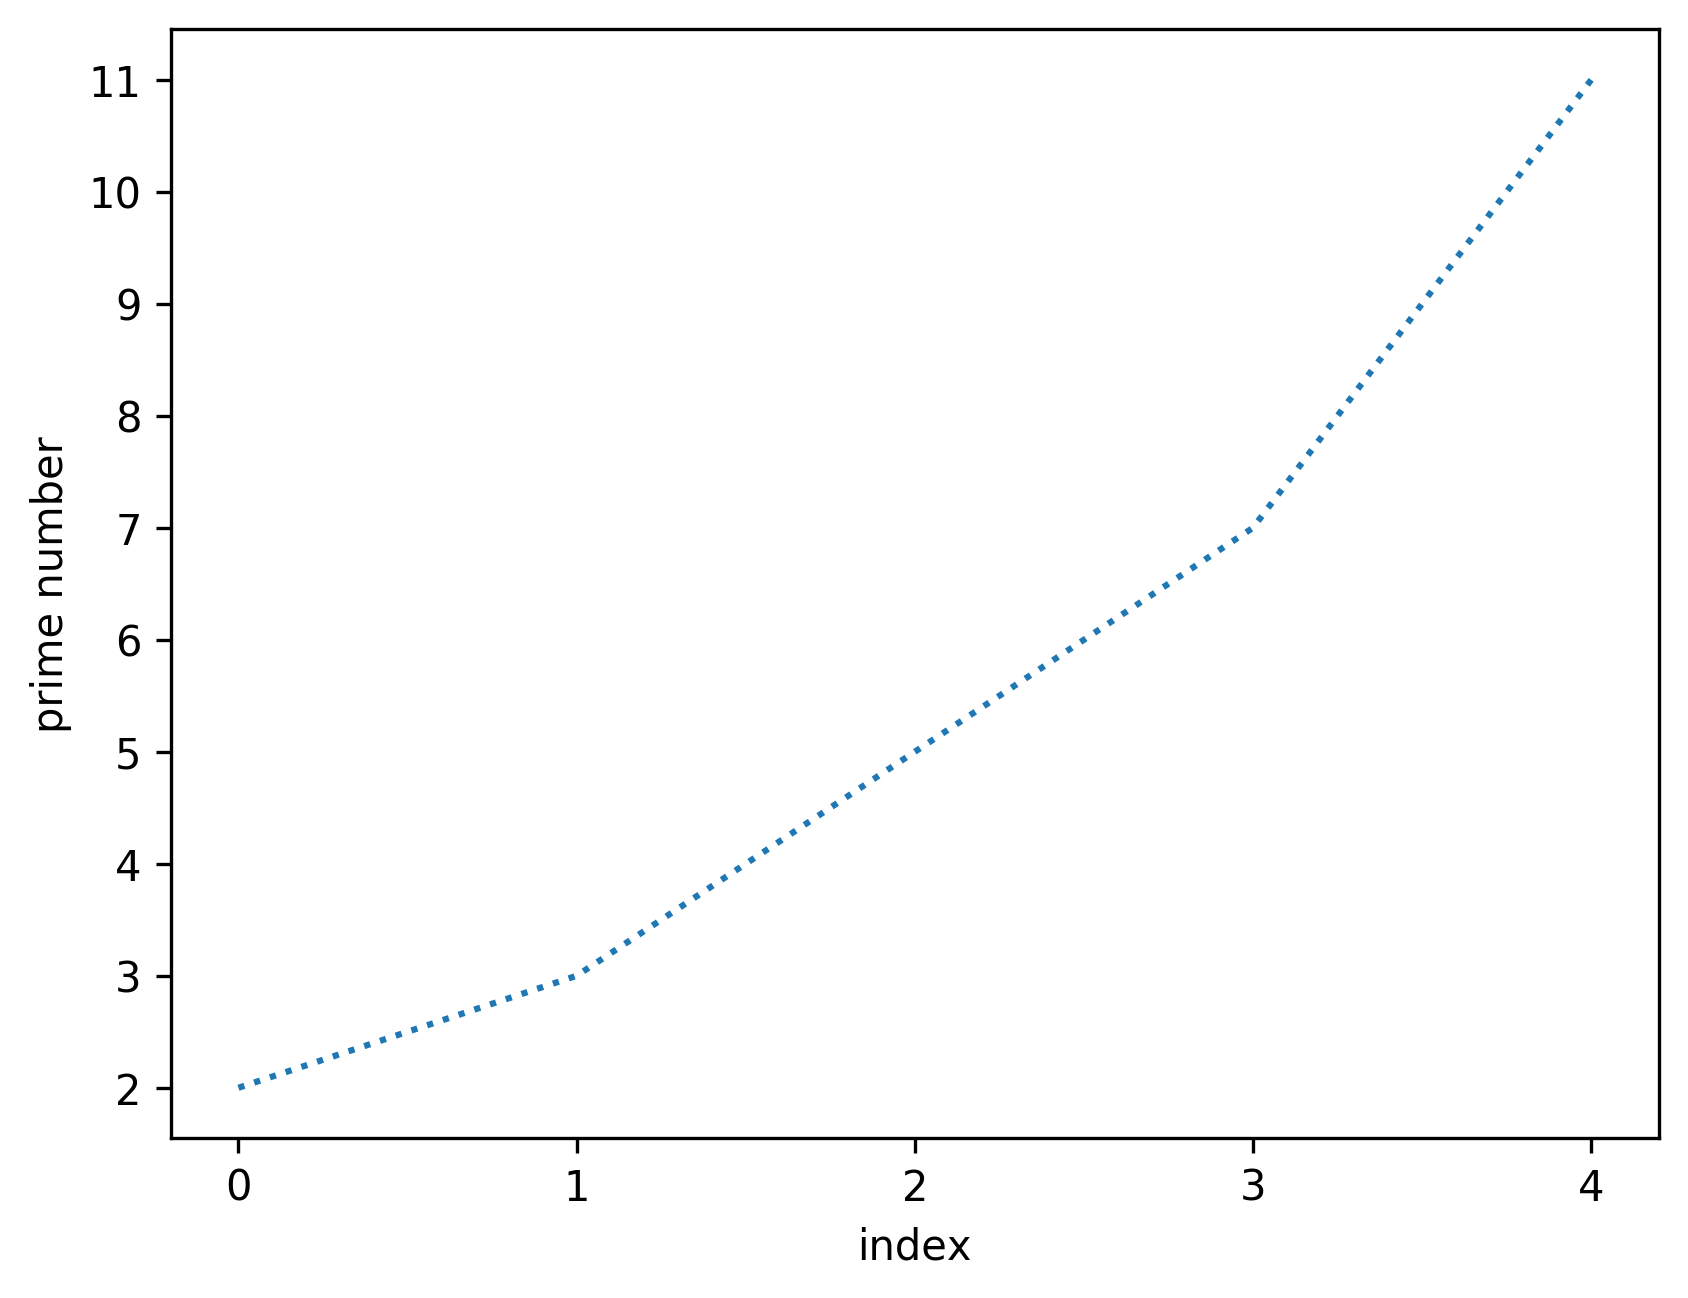
\includegraphics[width=\textwidth]{img/14-dotted-line-style.png}
        \end{column}
    \end{columns}
\end{frame}


% Line Styles Reference
\begin{frame}[t,fragile]
    \frametitle{Line Styles Reference}
    \vspace{5mm}
    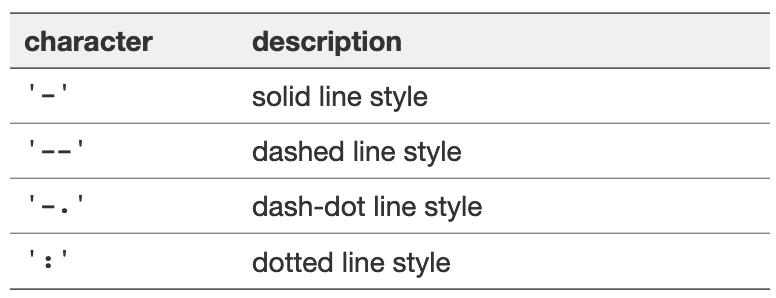
\includegraphics[width=0.75\textwidth]{img/ref-line-styles.png}

    \bigskip

    \footnotesize

    \hspace{0.2mm}
    Source:
    \url{https://matplotlib.org/api/_as_gen/matplotlib.pyplot.plot.html}
\end{frame}


% Bar Chart
\begin{frame}[t,fragile]
    \frametitle{Bar Chart}
    \vspace{-2mm}
    \begin{columns}[T]
        \begin{column}{0.54\textwidth}
            \pyfile[style=footnotesize]{examples/15-bar-simple.py}
        \end{column}
        \begin{column}{0.46\textwidth}
            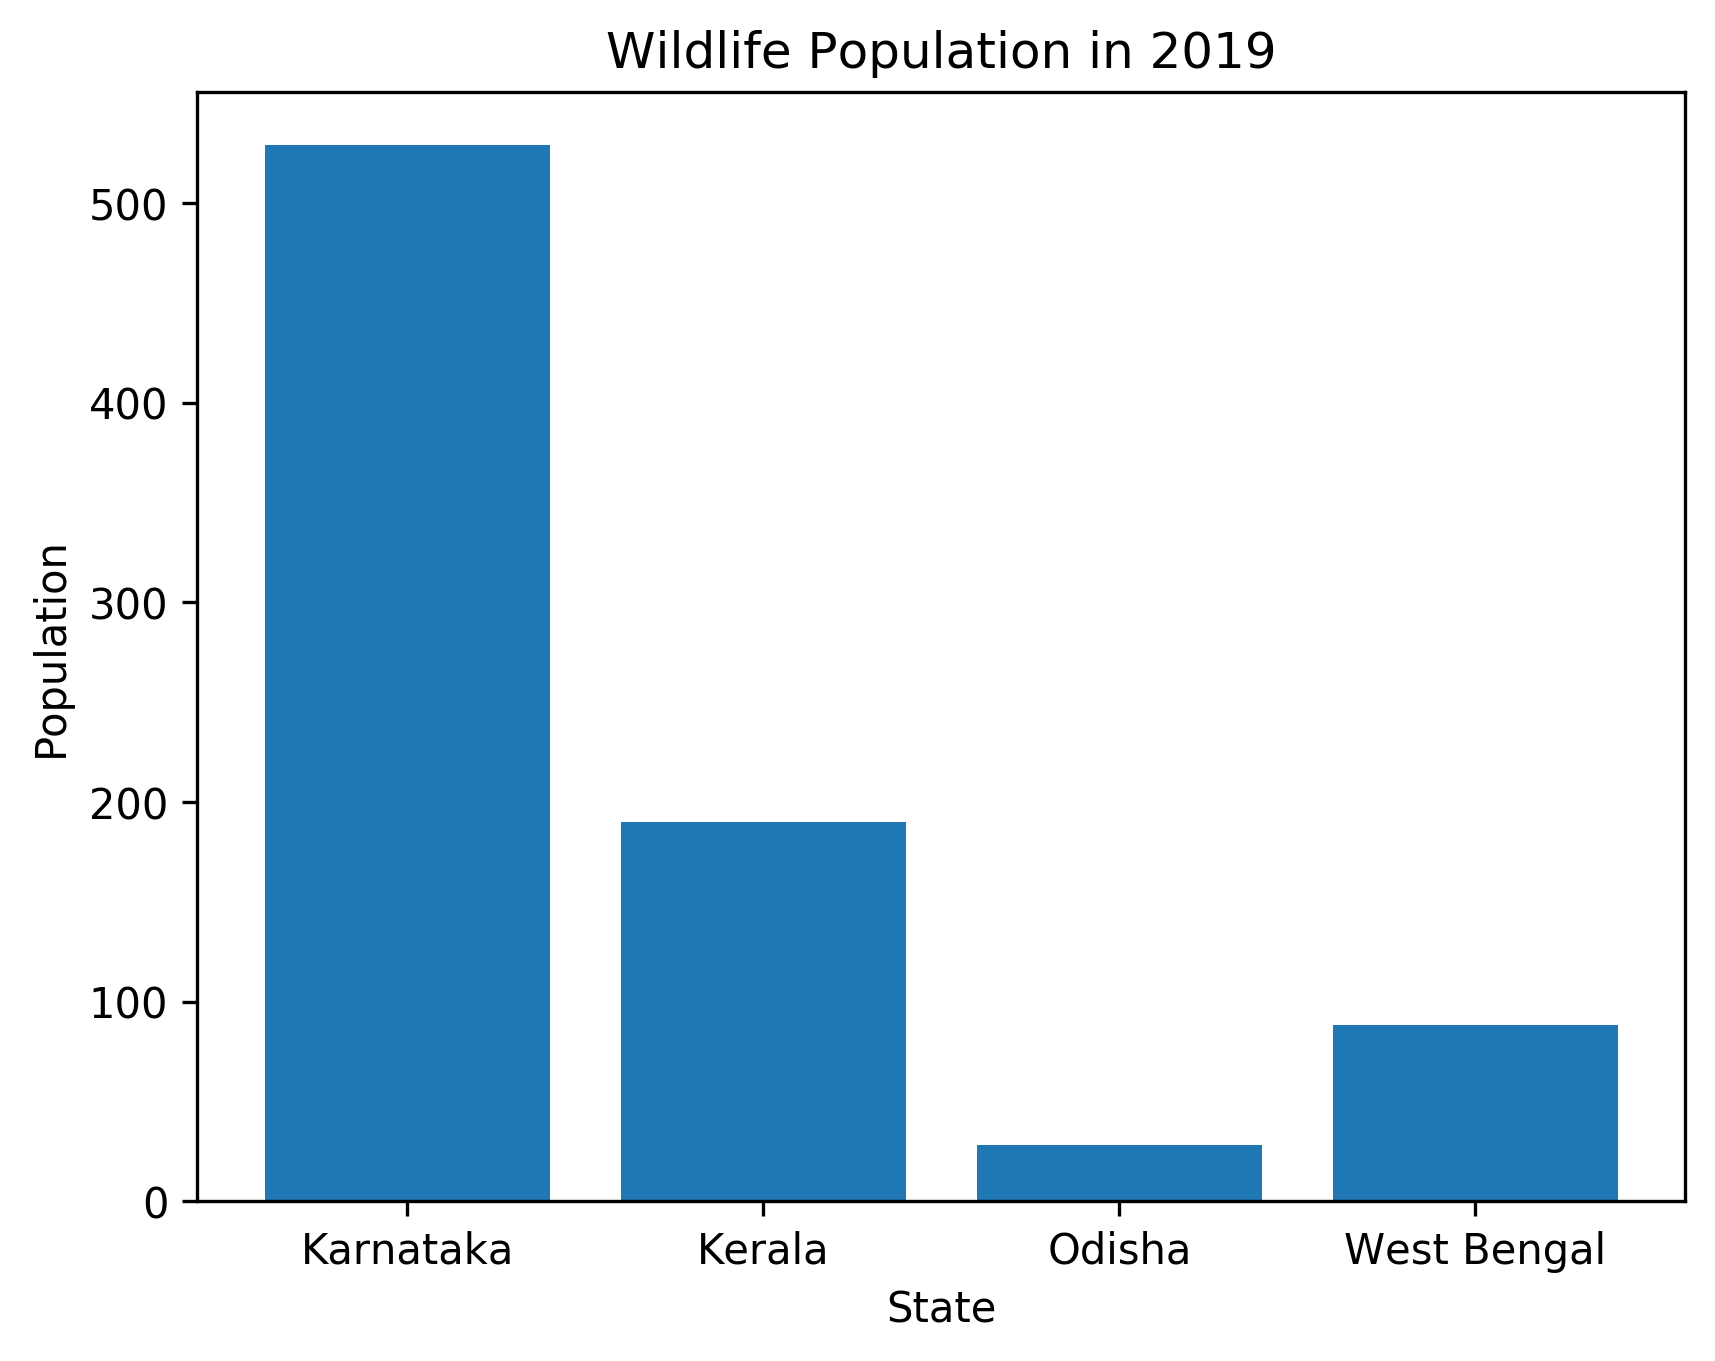
\includegraphics[width=\textwidth]{img/15-bar-simple.png}
        \end{column}
    \end{columns}
\end{frame}


% Bar Chart: Legend
\begin{frame}[t,fragile]
    \frametitle{Bar Chart: Legend}
    \vspace{-2mm}
    \begin{columns}[T]
        \begin{column}{0.54\textwidth}
            \pyfile[style=footnotesize]{examples/16-bar-legend.py}
        \end{column}
        \begin{column}{0.46\textwidth}
            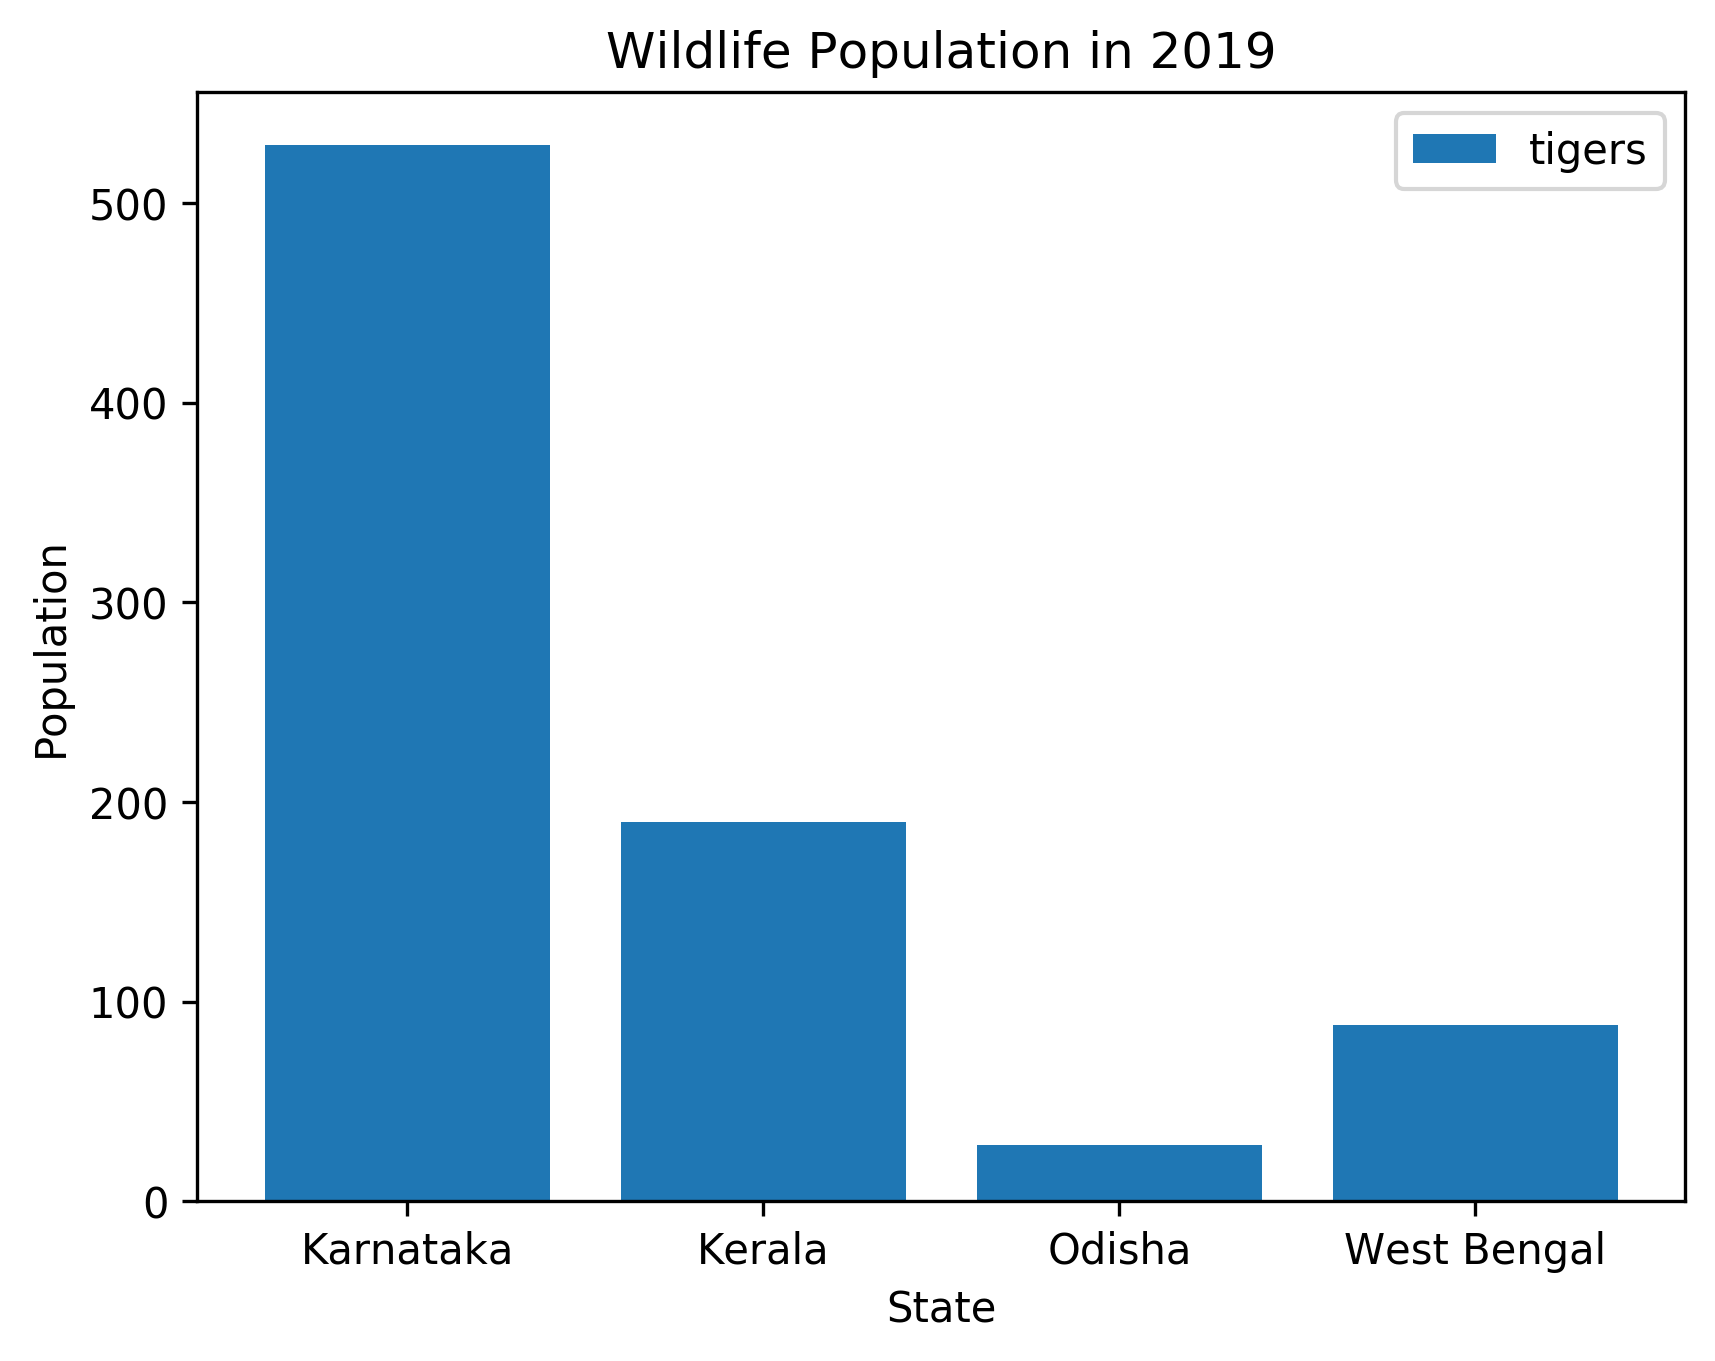
\includegraphics[width=\textwidth]{img/16-bar-legend.png}
        \end{column}
    \end{columns}
\end{frame}


% Bar Chart: Using plt.text() to Display Values
\begin{frame}[t,fragile]
    \frametitle{Bar Chart: Using \ttcode{plt.text()} to Display Values}
    \vspace{-2mm}
    \begin{columns}[T]
        \begin{column}{0.54\textwidth}
            \pyfile[style=footnotesize]{examples/17-bar-values-misaligned.py}
        \end{column}
        \begin{column}{0.46\textwidth}
            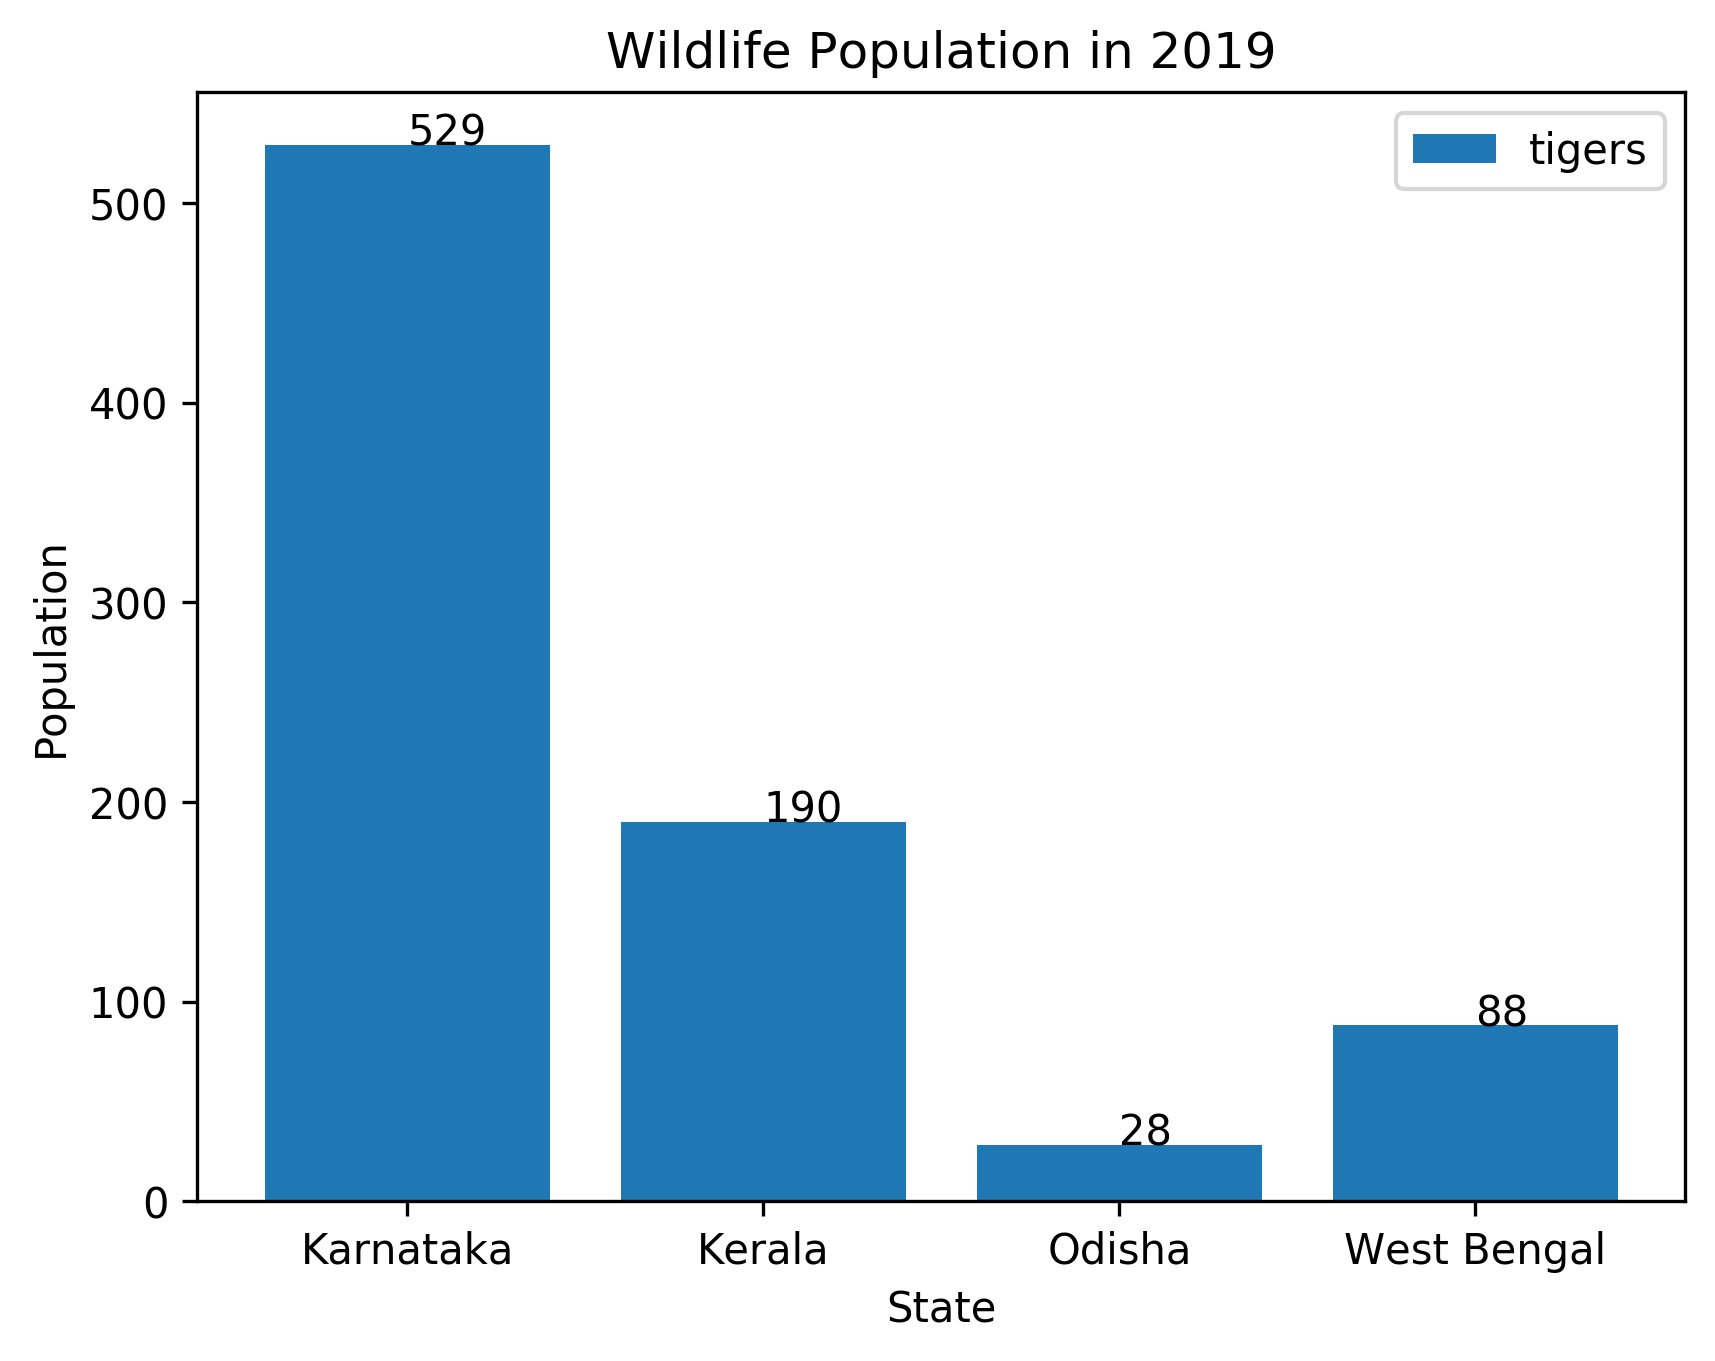
\includegraphics[width=\textwidth]{img/17-bar-values-misaligned.png}
        \end{column}
    \end{columns}
\end{frame}


% Bar Chart: Center the Values on the Bars
\begin{frame}[t,fragile]
    \frametitle{Bar Chart: Center the Values on the Bars}
    \vspace{-2mm}
    \begin{columns}[T]
        \begin{column}{0.54\textwidth}
            \pyfile[style=footnotesize]{examples/18-bar-values-aligned.py}
        \end{column}
        \begin{column}{0.46\textwidth}
            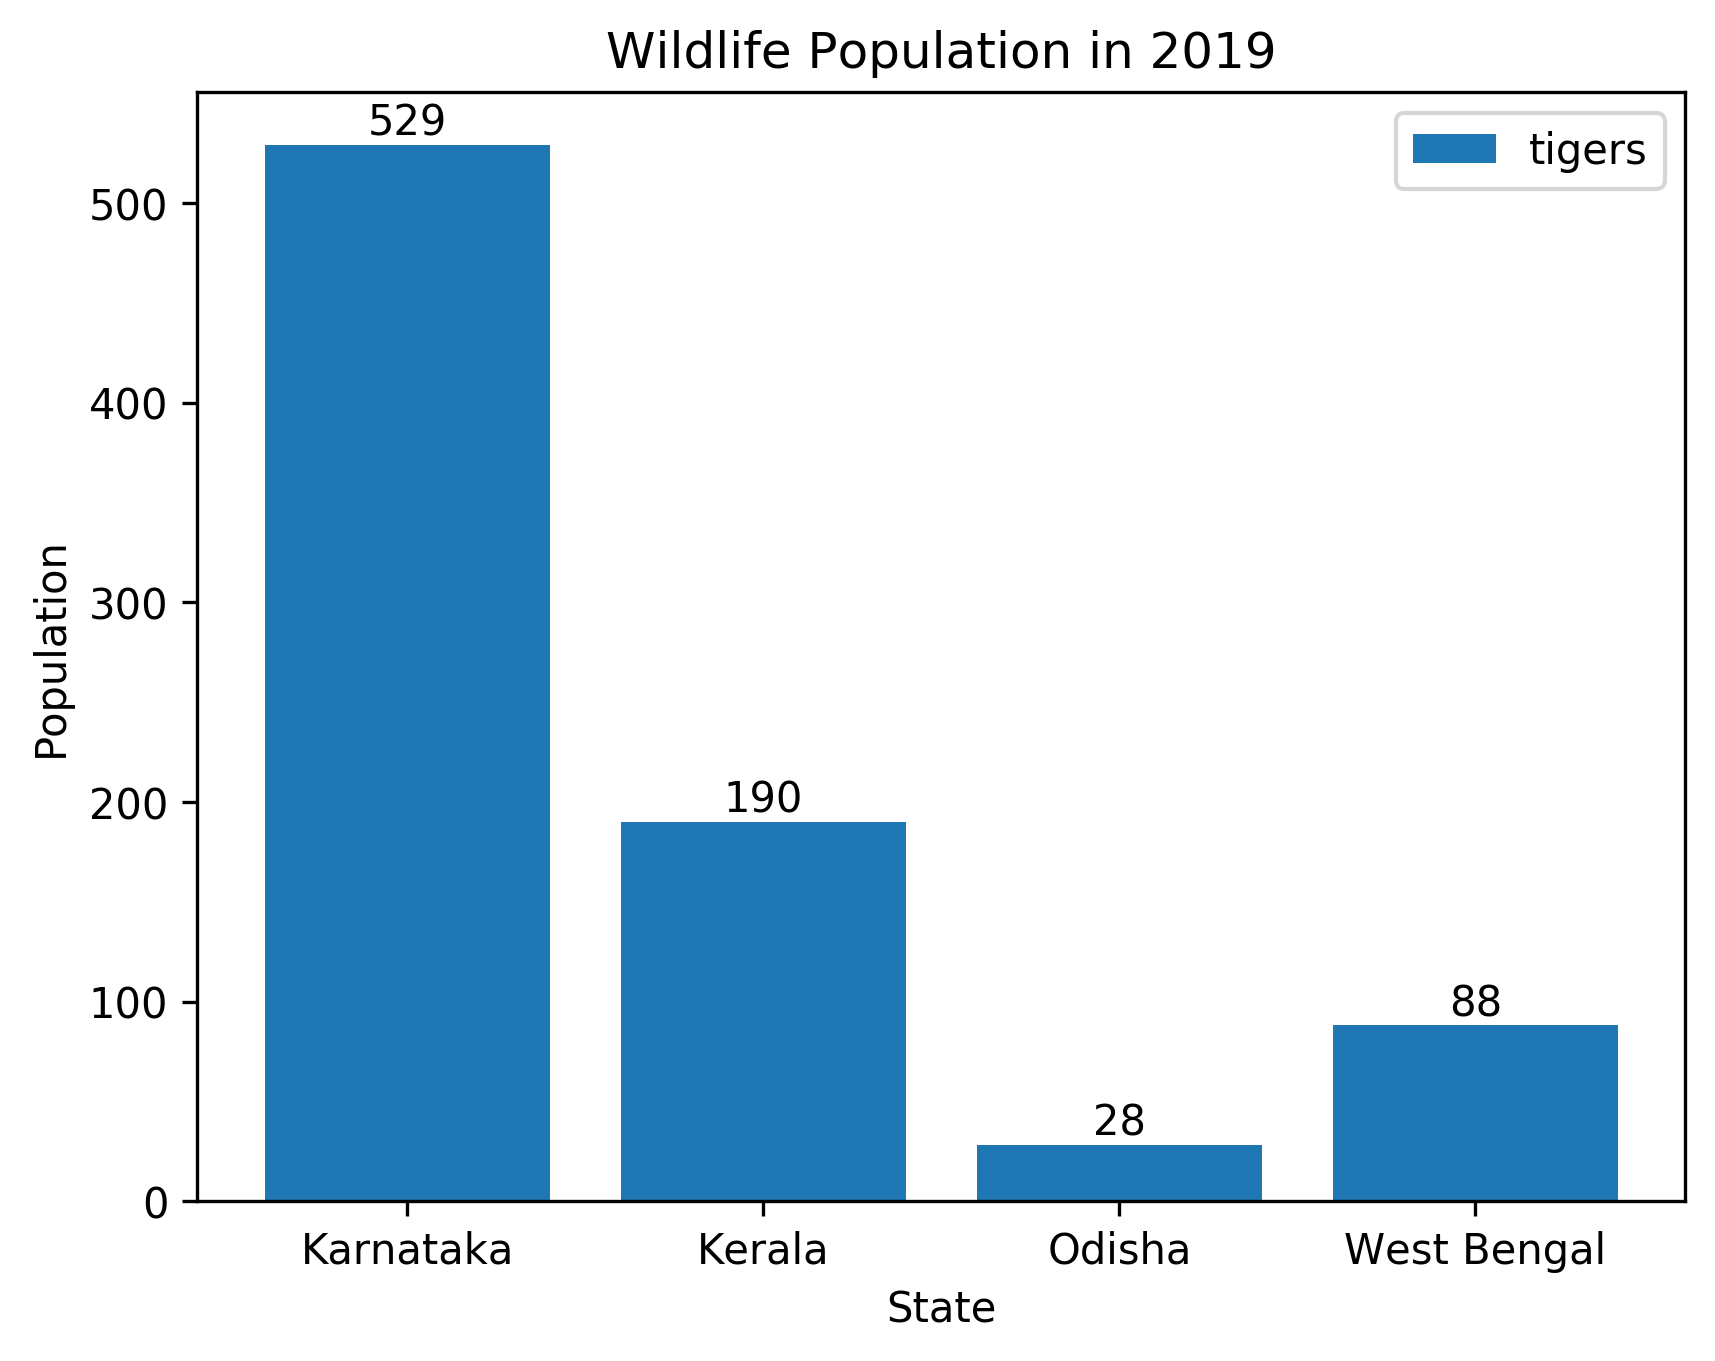
\includegraphics[width=\textwidth]{img/18-bar-values-aligned.png}
        \end{column}
    \end{columns}
\end{frame}


% Grouped Bar Chart
\begin{frame}[t,fragile]
    \frametitle{Grouped Bar Chart}
    \vspace{-2mm}
    \begin{columns}[T]
        \begin{column}{0.54\textwidth}
            \pyfile[style=tiny]{examples/19-bar-grouped.py}
        \end{column}
        \begin{column}{0.46\textwidth}
            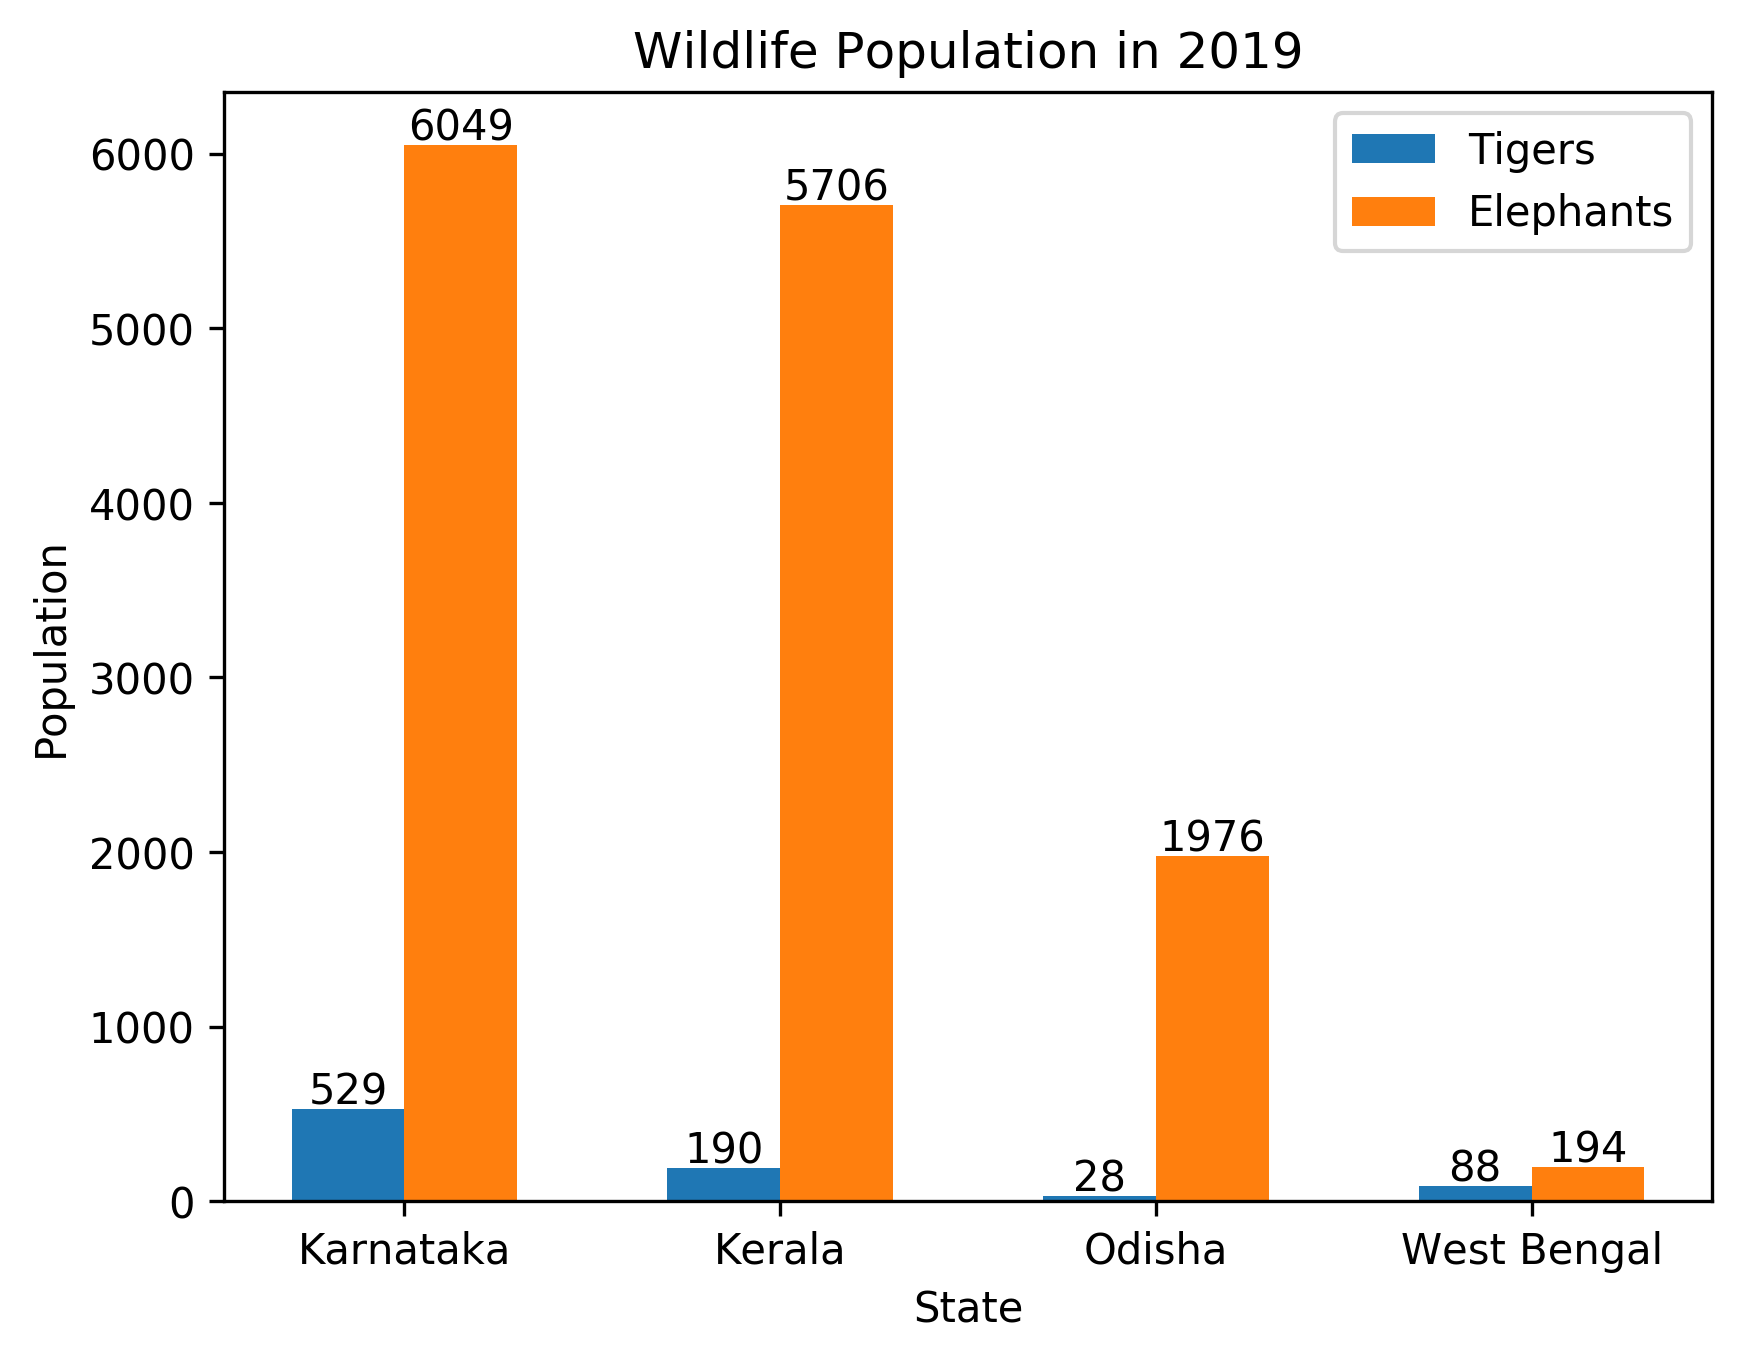
\includegraphics[width=\textwidth]{img/19-bar-grouped.png}
        \end{column}
    \end{columns}
\end{frame}


% Stacked Bar Chart
\begin{frame}[t,fragile]
    \frametitle{Stacked Bar Chart}
    \vspace{-2mm}
    \begin{columns}[T]
        \begin{column}{0.54\textwidth}
            \pyfile[style=scriptsize]{examples/20-bar-stacked.py}
        \end{column}
        \begin{column}{0.46\textwidth}
            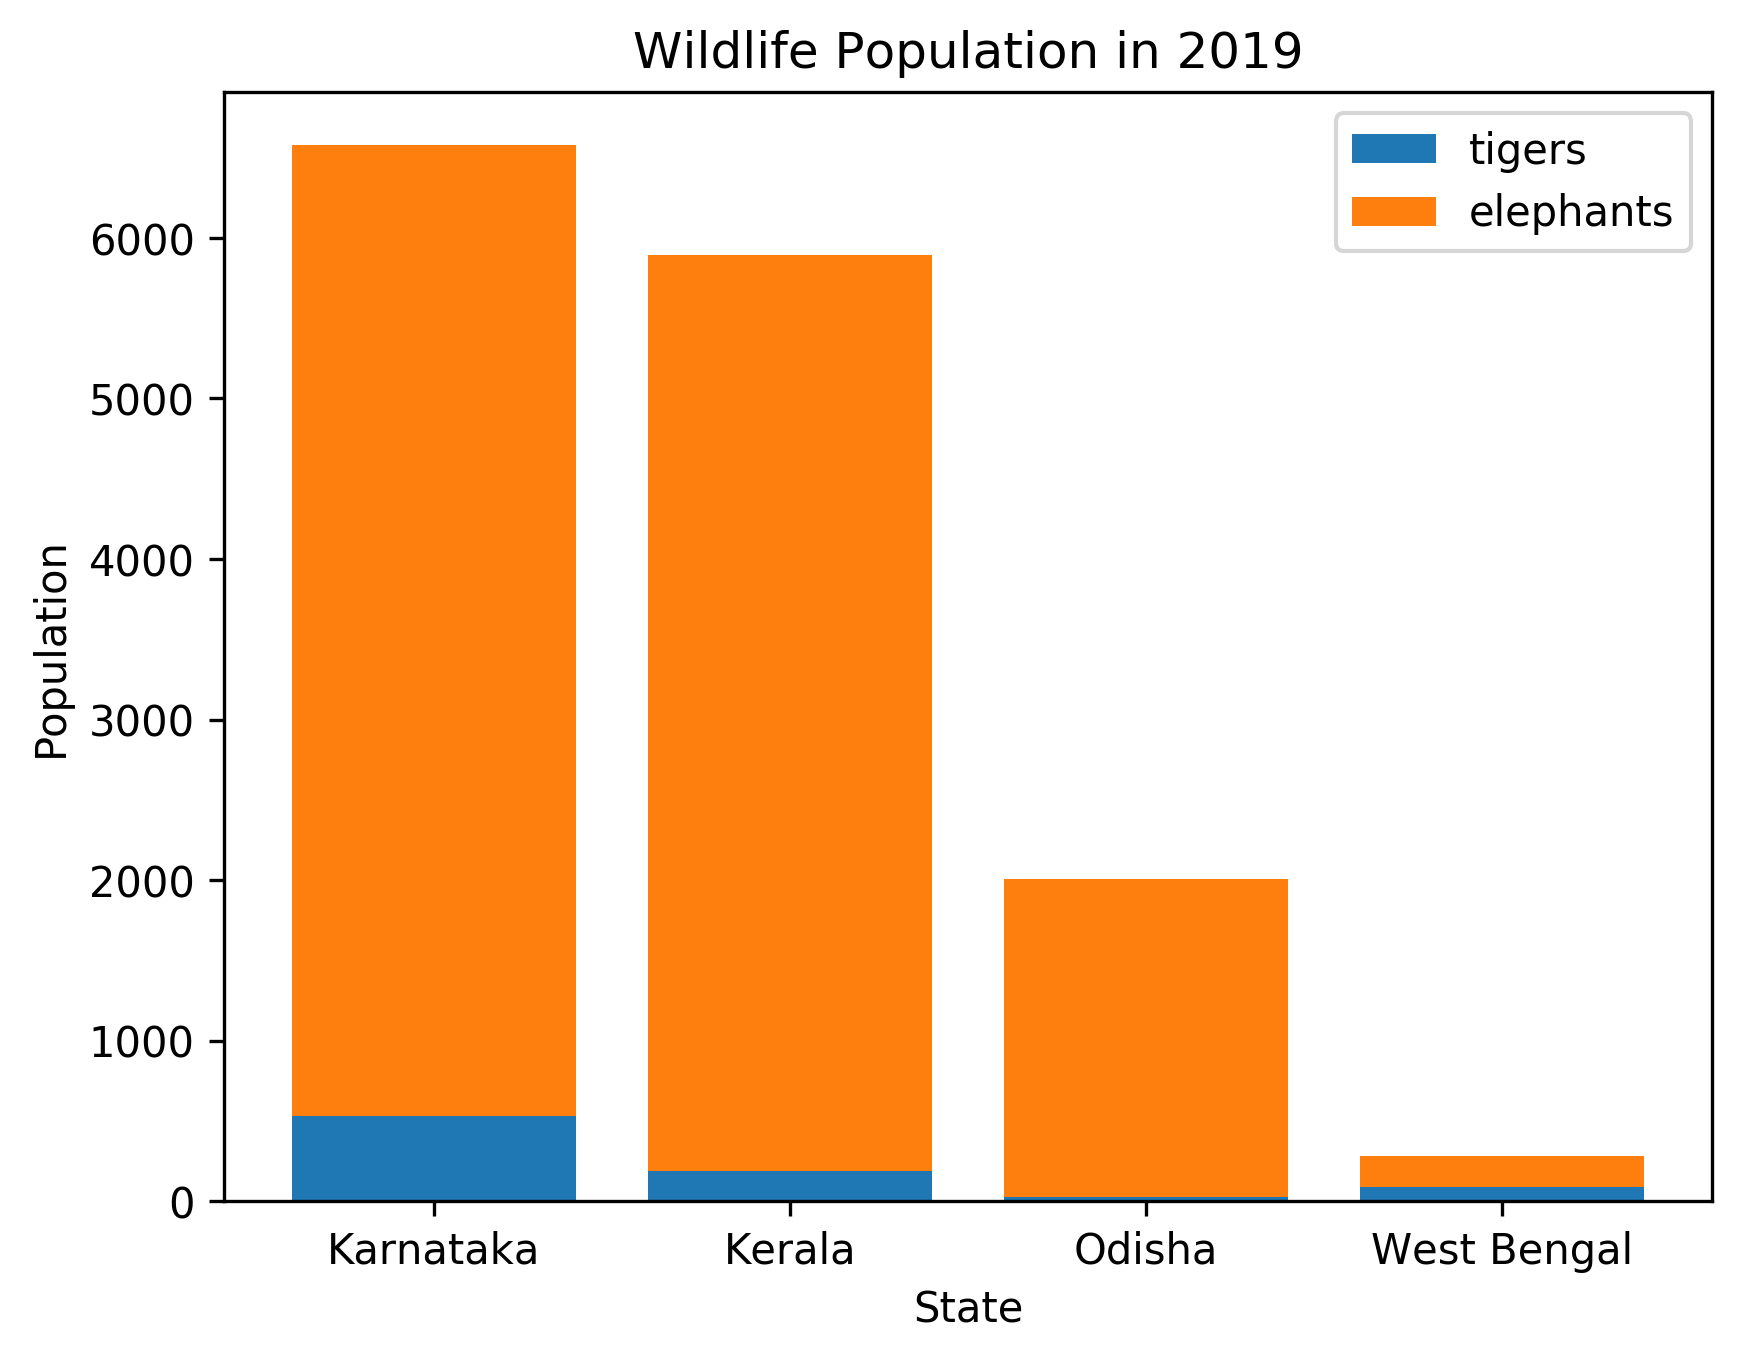
\includegraphics[width=\textwidth]{img/20-bar-stacked.png}
        \end{column}
    \end{columns}
\end{frame}


% Heart Plot: The Equations
\begin{frame}
    \frametitle{Heart Plot: The Equations}

    \begin{align*}
        y_1 & = \sqrt{1 - |x|} \sqrt{|x|}, \\
        y_2 & = -\frac{3}{2} \sqrt{1 - \sqrt{|x|}}.
    \end{align*}

    \bigskip

    \bigskip

    \begin{center}
        See \url{https://github.com/susam/heart} for more details.
    \end{center}
\end{frame}


% Heart Plot: Plot the Equations
\begin{frame}[t,fragile]
    \frametitle{Heart Plot: Plot the Equations}
    \vspace{-2mm}
    \begin{columns}[T]
        \begin{column}{0.47\textwidth}
            \pyfile[style=tiny,linerange={1-18}]{examples/heart-0.py}
        \end{column}
        \begin{column}{0.53\textwidth}
            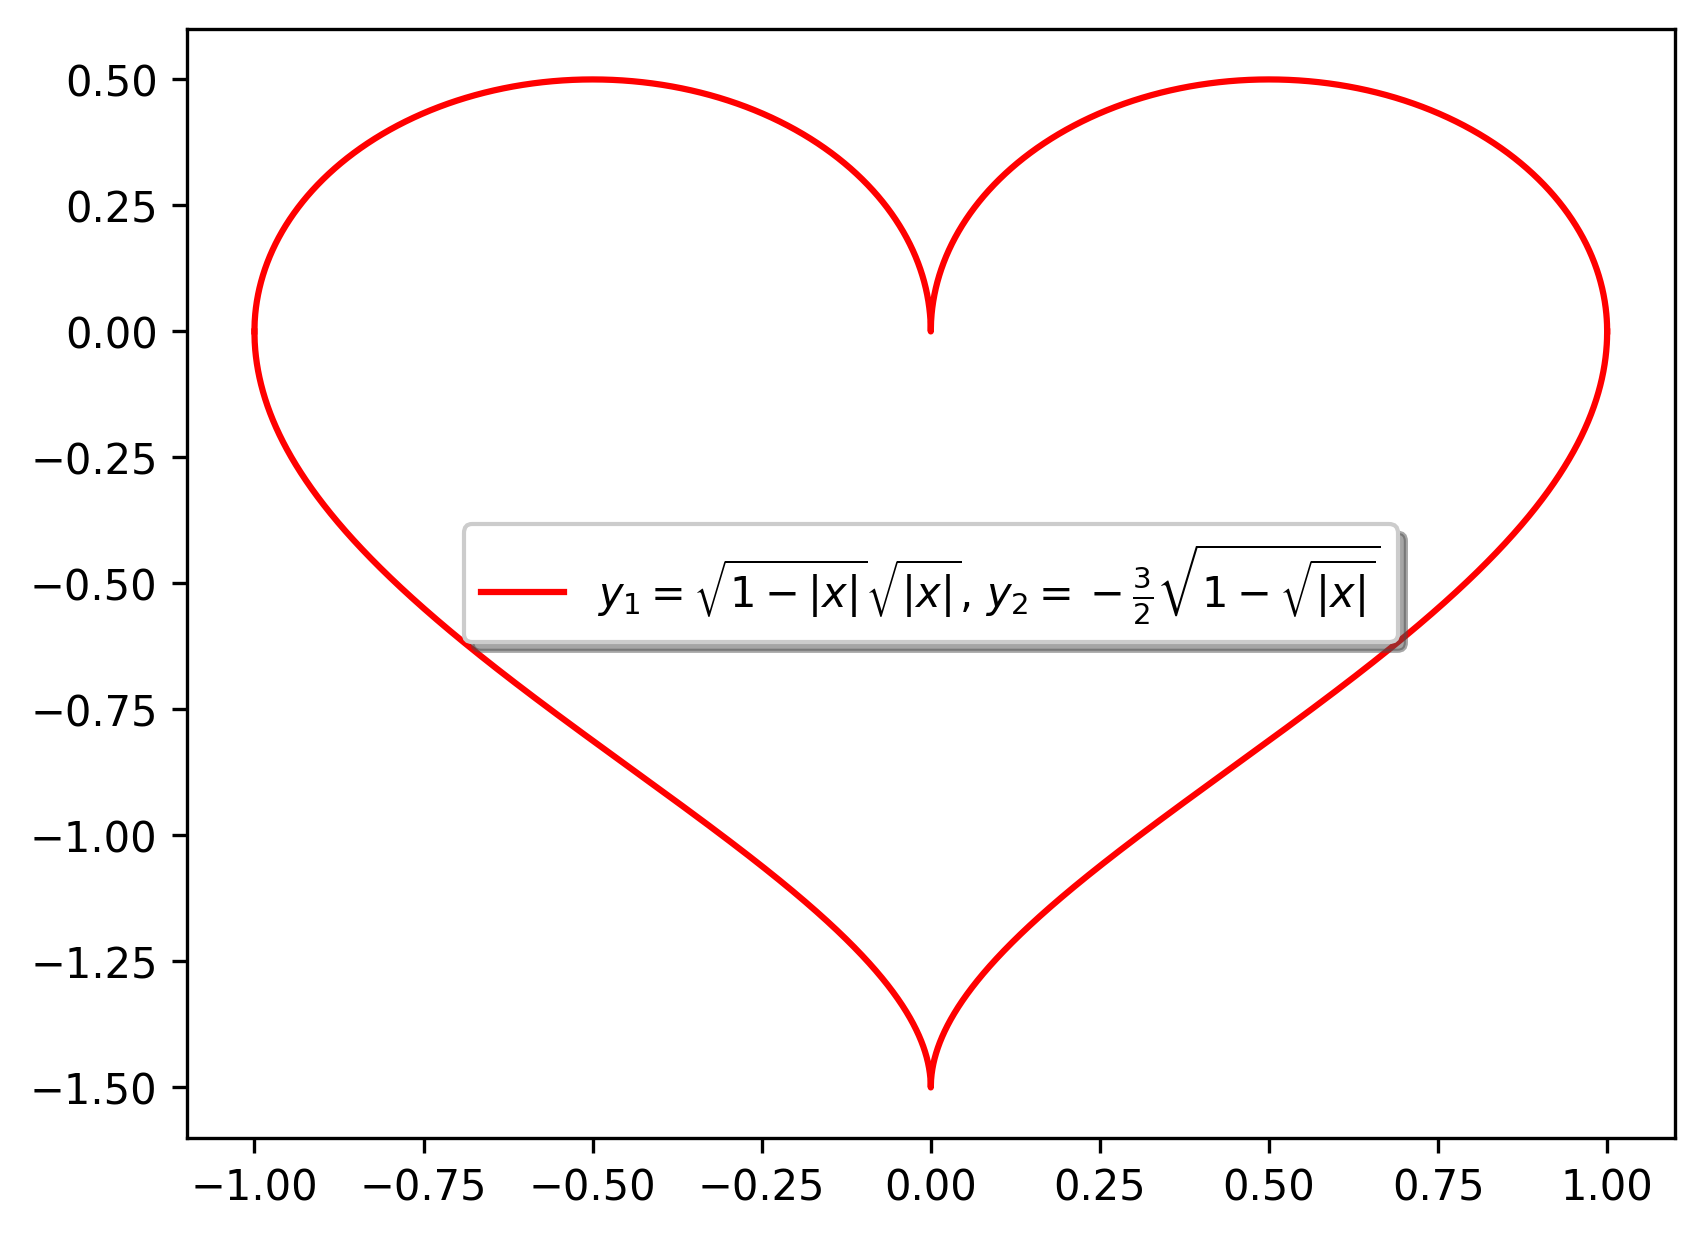
\includegraphics[width=\textwidth]{img/heart-0.png}
        \end{column}
    \end{columns}
\end{frame}


% Heart Plot: X and Y Limits
\begin{frame}[t,fragile]
    \frametitle{Heart Plot: X and Y Limits}
    \vspace{-2mm}
    \begin{columns}[T]
        \begin{column}{0.47\textwidth}
            \pyfile[style=tiny,linerange={1-22}]{examples/heart-1.py}
        \end{column}
        \begin{column}{0.53\textwidth}
            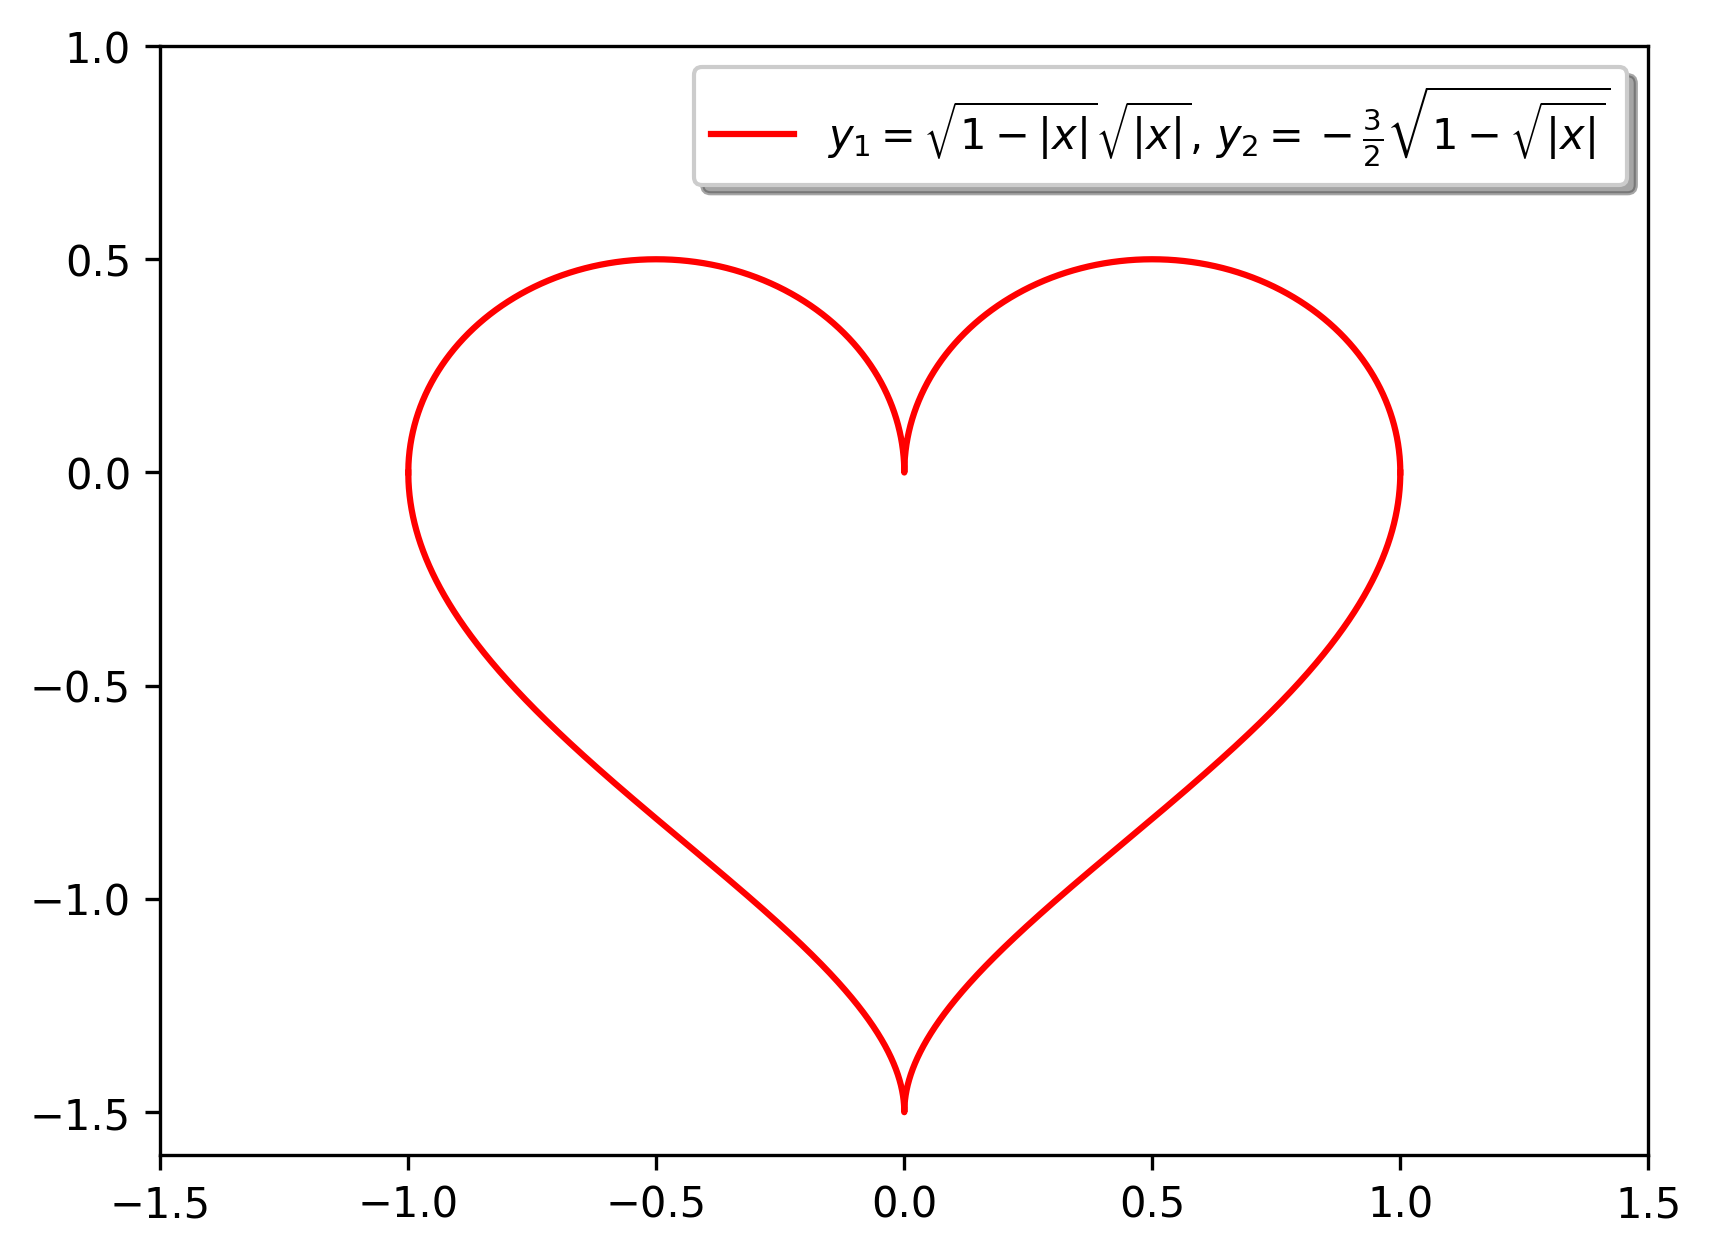
\includegraphics[width=\textwidth]{img/heart-1.png}
        \end{column}
    \end{columns}
\end{frame}


% Heart Plot: Major and Minor Tick Locations
\begin{frame}[t,fragile]
    \frametitle{Heart Plot: Major and Minor Tick Locations}
    \vspace{-2mm}
    \begin{columns}[T]
        \begin{column}{0.47\textwidth}
            \pyfile[style=tiny]{examples/heart-2.py}
        \end{column}
        \begin{column}{0.53\textwidth}
            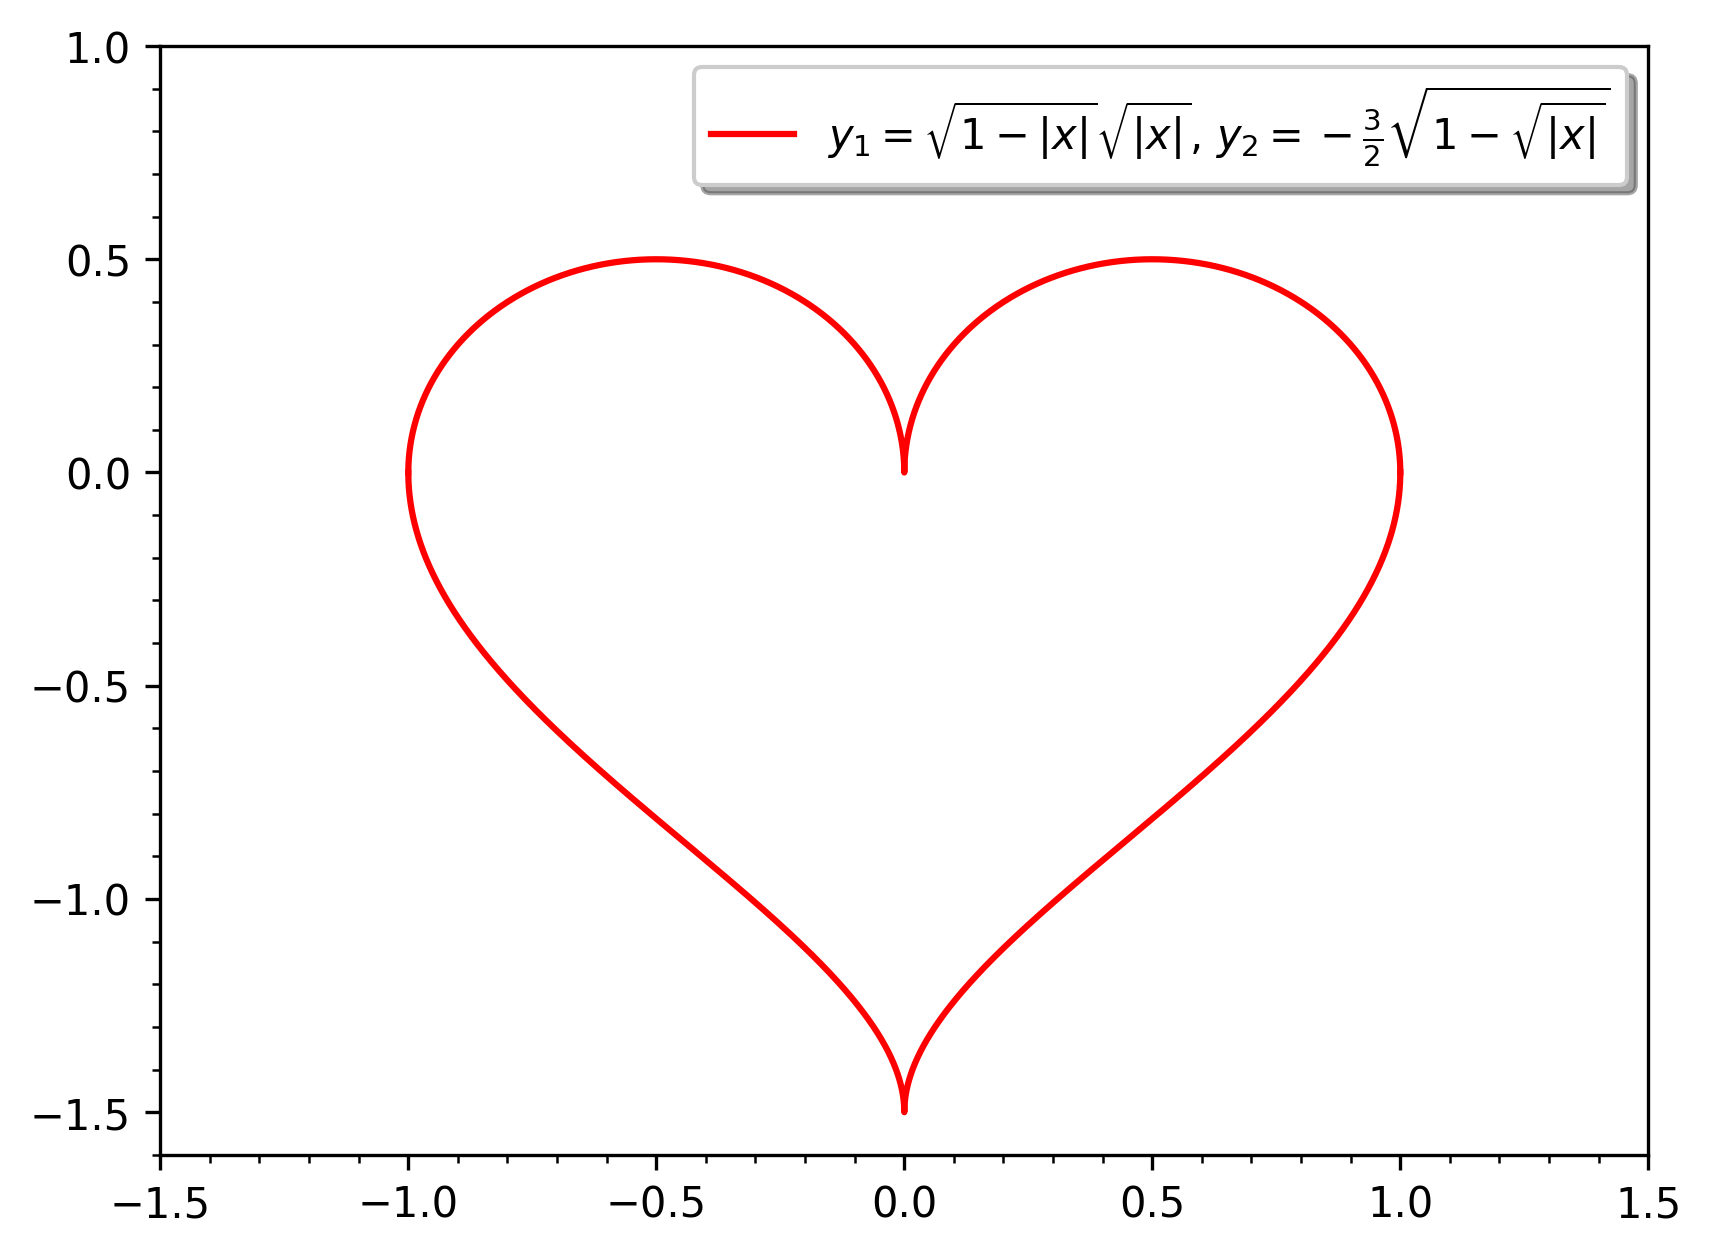
\includegraphics[width=\textwidth]{img/heart-2.png}
        \end{column}
    \end{columns}
\end{frame}

% Heart Plot: Green Color Grid
\begin{frame}[t,fragile]
    \frametitle{Heart Plot: Green Color Grid}
    \vspace{-2mm}
    \begin{columns}[T]
        \begin{column}{0.47\textwidth}
            \pyfile[style=tiny,linerange=30]{examples/heart-3.py}
        \end{column}
        \begin{column}{0.53\textwidth}
            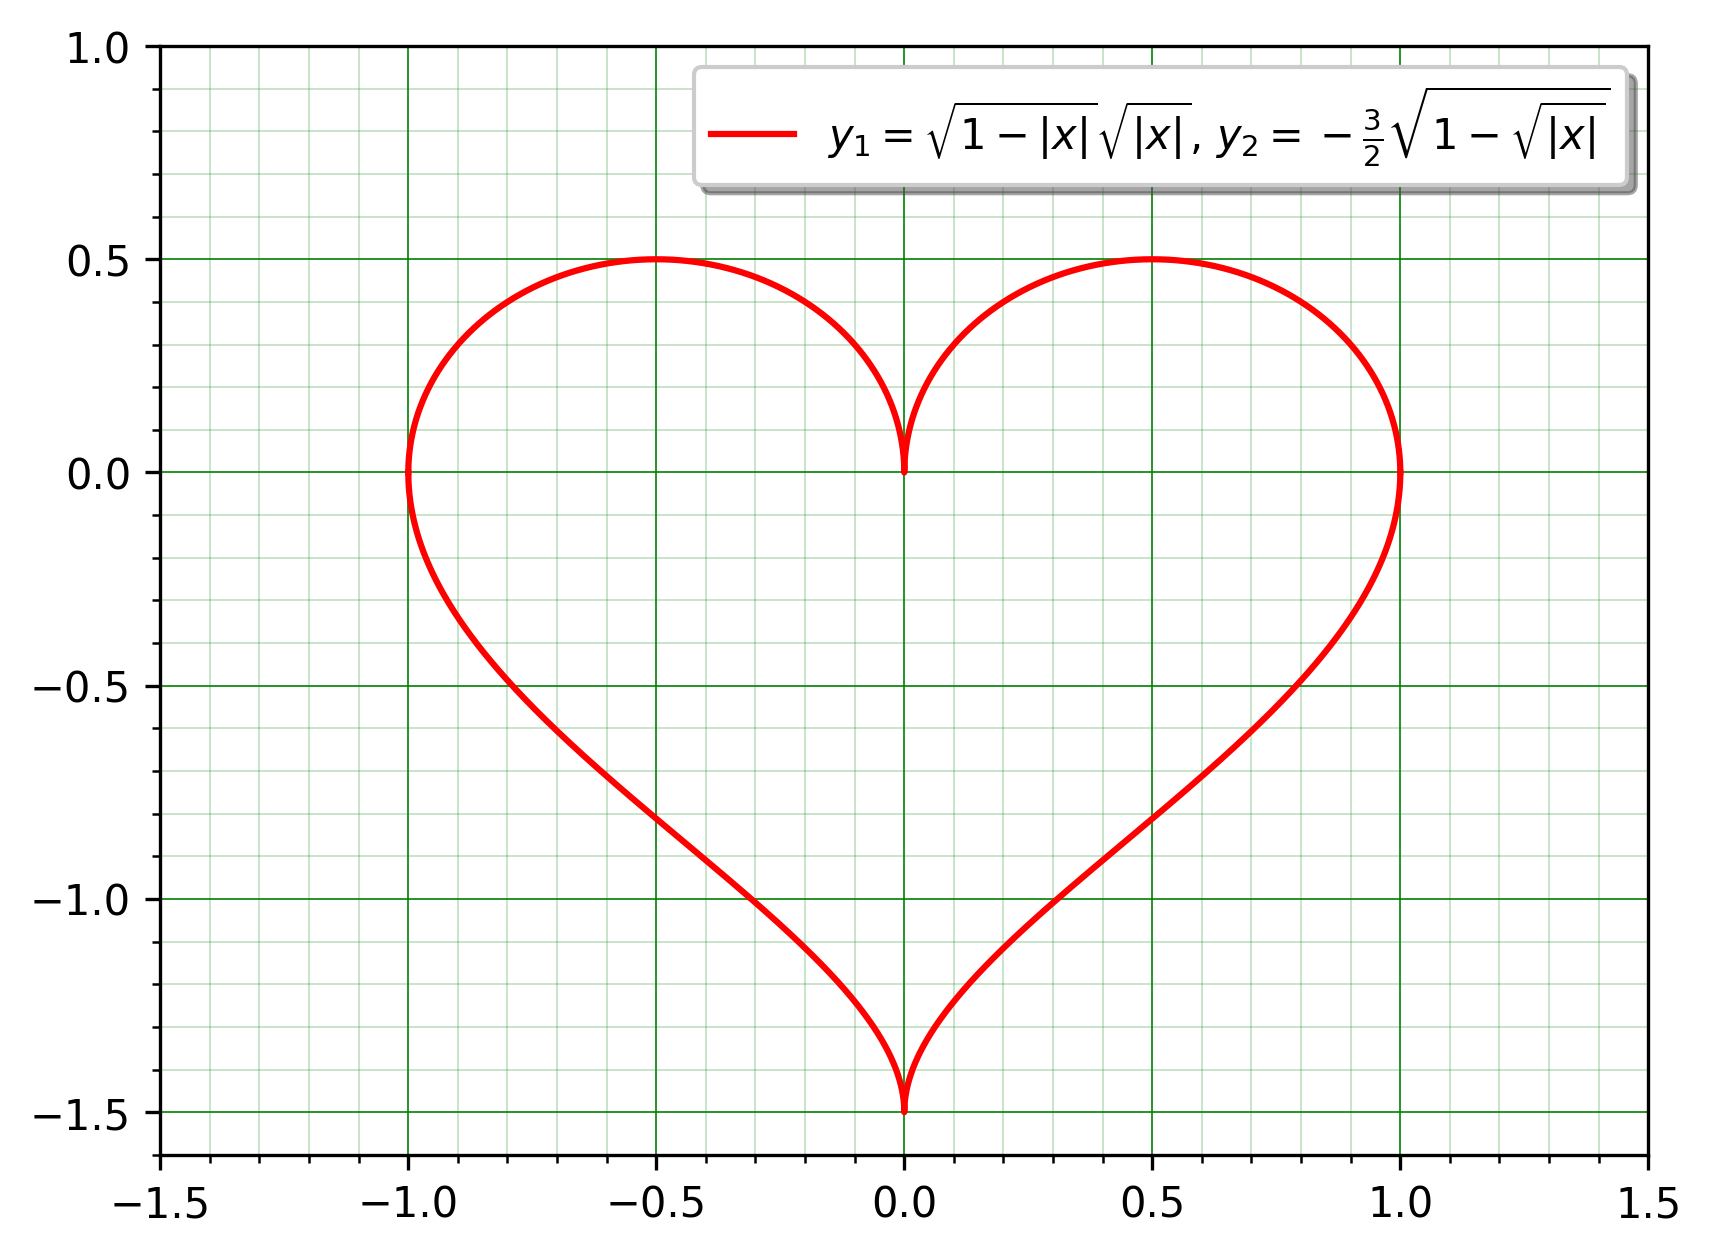
\includegraphics[width=\textwidth]{img/heart-3.png}
        \end{column}
    \end{columns}
\end{frame}


% Heart Plot: Green Color Ticks
\begin{frame}[t,fragile]
    \frametitle{Heart Plot: Green Color Ticks}
    \vspace{-2mm}
    \begin{columns}[T]
        \begin{column}{0.47\textwidth}
            \pyfile[style=tiny,linerange=30]{examples/heart-4.py}
        \end{column}
        \begin{column}{0.53\textwidth}
            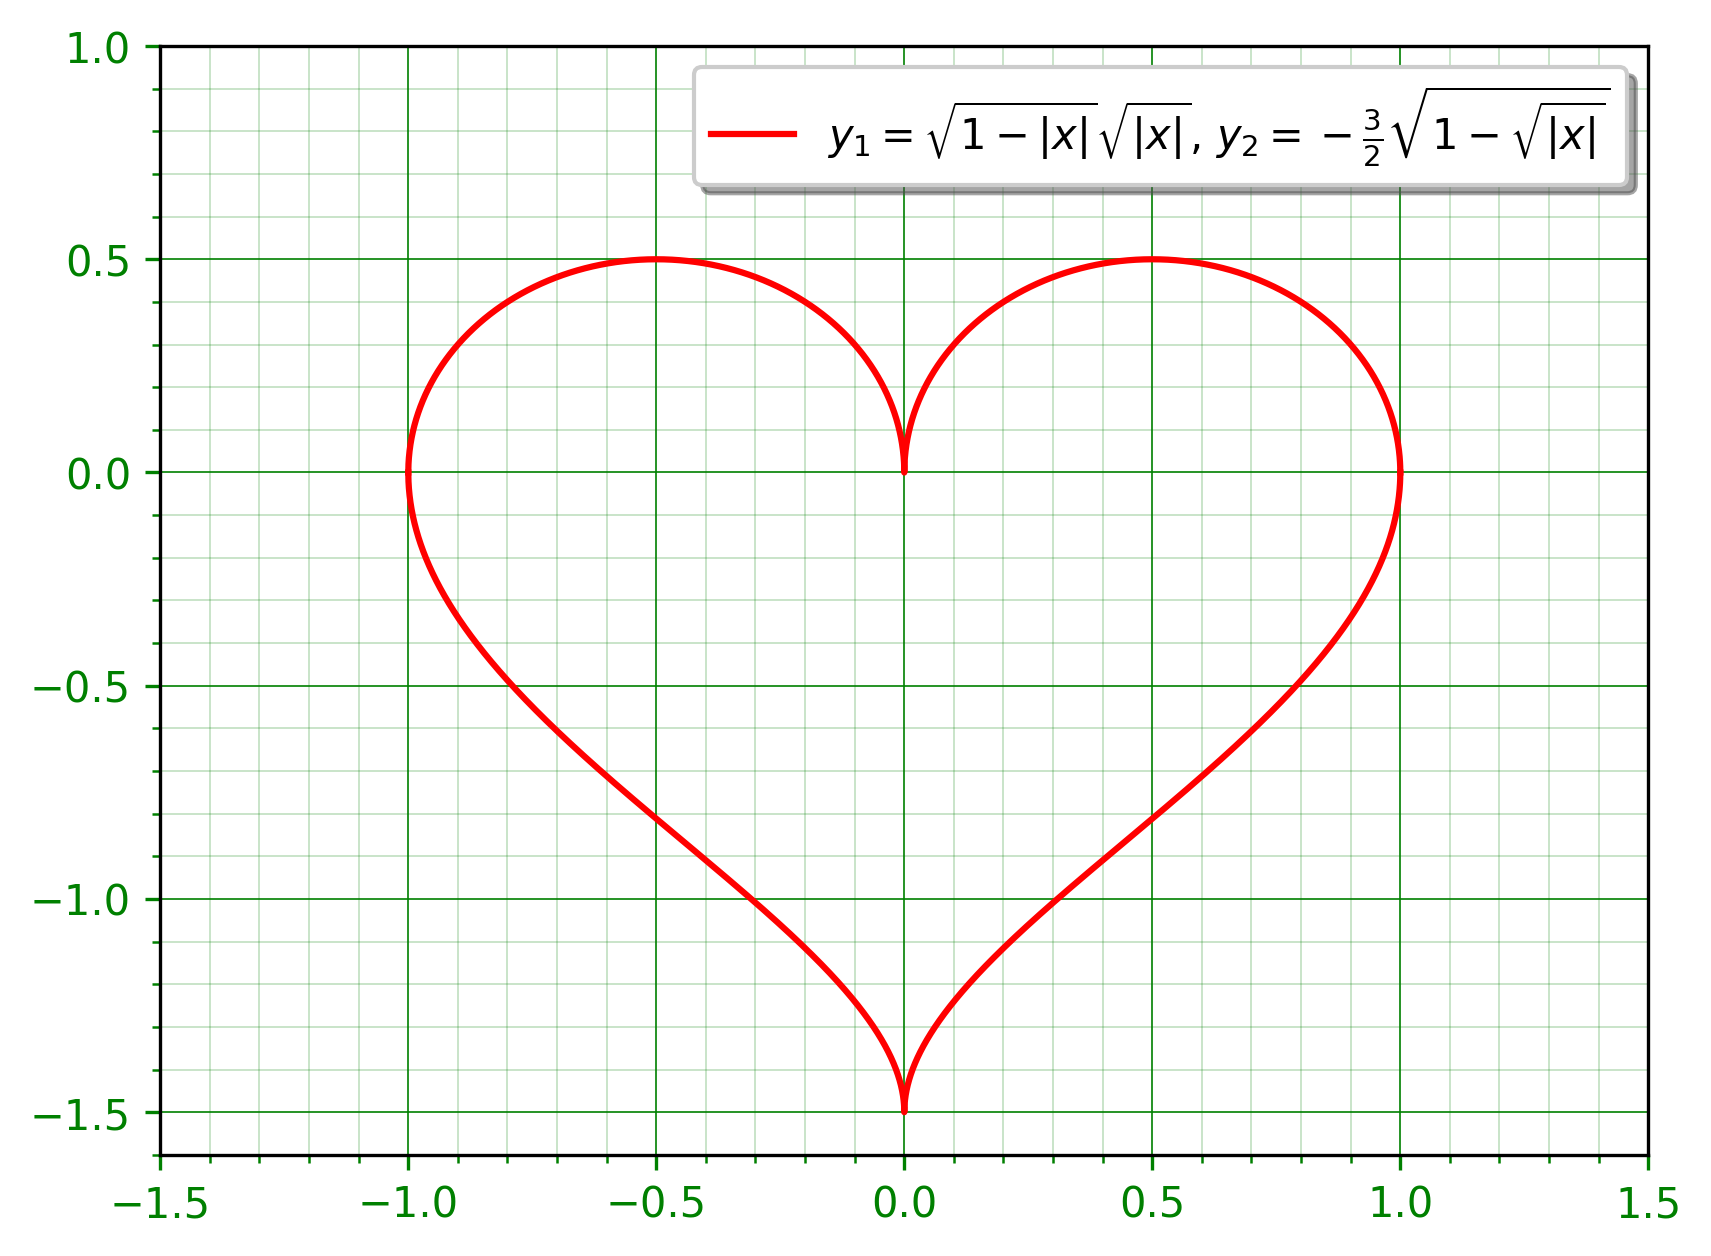
\includegraphics[width=\textwidth]{img/heart-4.png}
        \end{column}
    \end{columns}
\end{frame}


% Heart Plot: Zero Tick Length
\begin{frame}[t,fragile]
    \frametitle{Heart Plot: Zero Tick Length}
    \vspace{-2mm}
    \begin{columns}[T]
        \begin{column}{0.47\textwidth}
            \pyfile[style=tiny,linerange=30]{examples/heart-5.py}
        \end{column}
        \begin{column}{0.53\textwidth}
            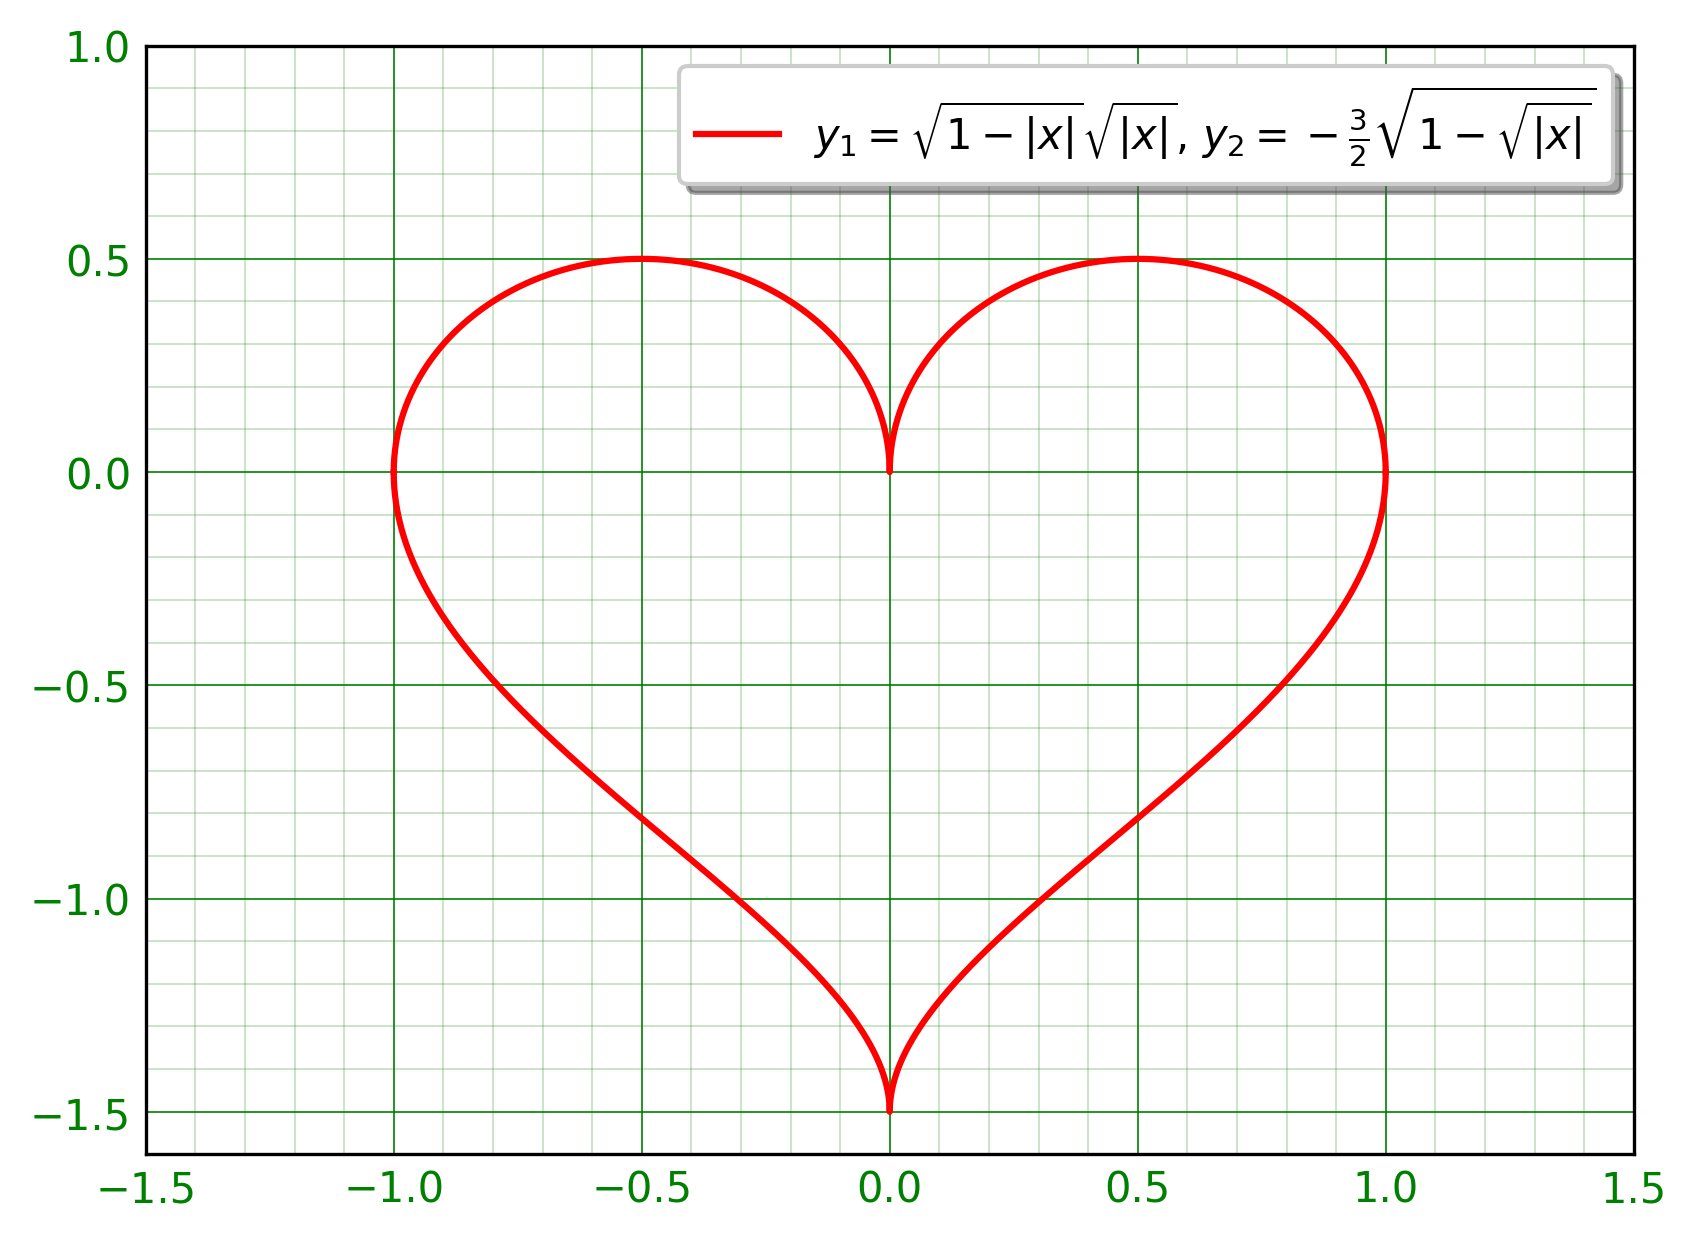
\includegraphics[width=\textwidth]{img/heart-5.png}
        \end{column}
    \end{columns}
\end{frame}


% Heart Plot: Green Spines
\begin{frame}[t,fragile]
    \frametitle{Heart Plot: Green Spines}
    \vspace{-2mm}
    \begin{columns}[T]
        \begin{column}{0.47\textwidth}
            \pyfile[style=tiny,linerange=30]{examples/heart-6.py}
        \end{column}
        \begin{column}{0.53\textwidth}
            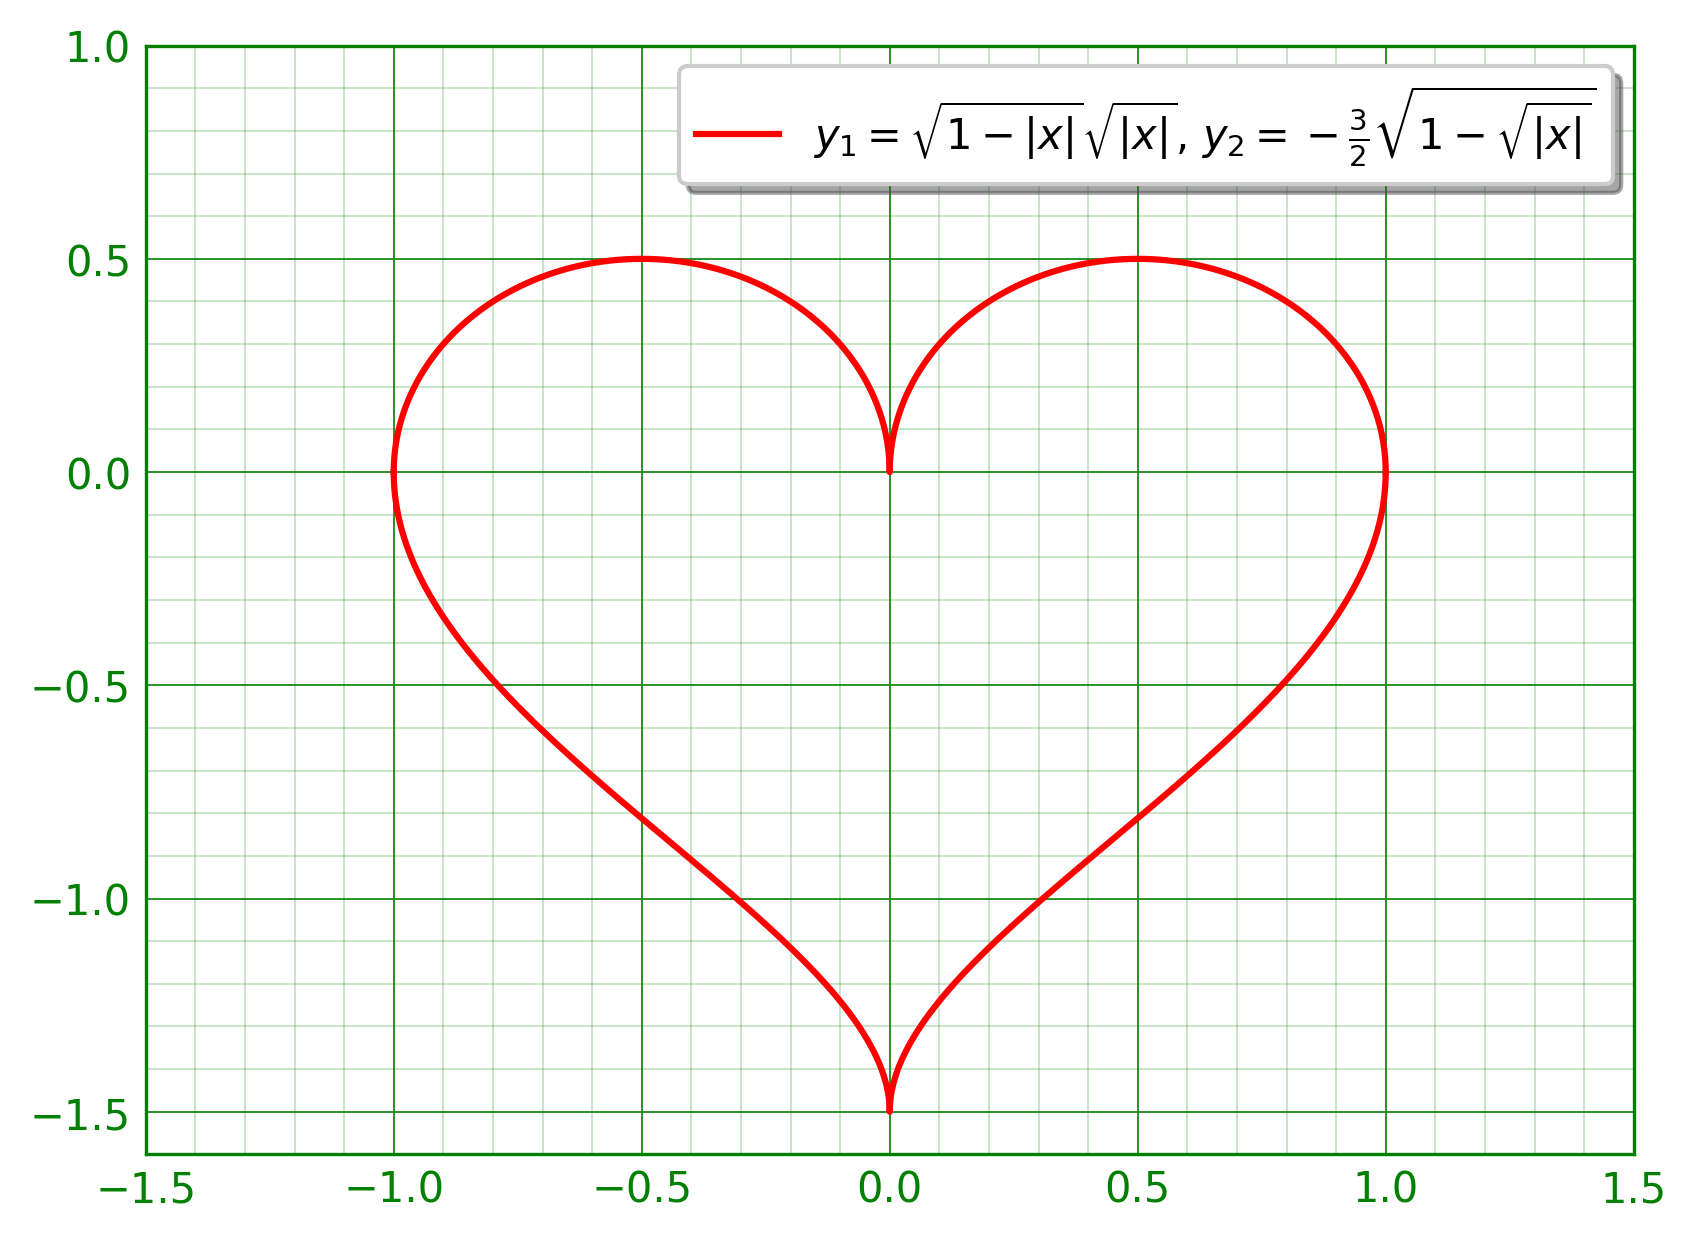
\includegraphics[width=\textwidth]{img/heart-6.png}
        \end{column}
    \end{columns}
\end{frame}


% Heart Plot: Equal Aspect Ratio
\begin{frame}[t,fragile]
    \frametitle{Heart Plot: Equal Aspect Ratio}
    \vspace{-2mm}
    \begin{columns}[T]
        \begin{column}{0.47\textwidth}
            \pyfile[style=tiny,linerange=30]{examples/heart-7.py}
        \end{column}
        \begin{column}{0.53\textwidth}
            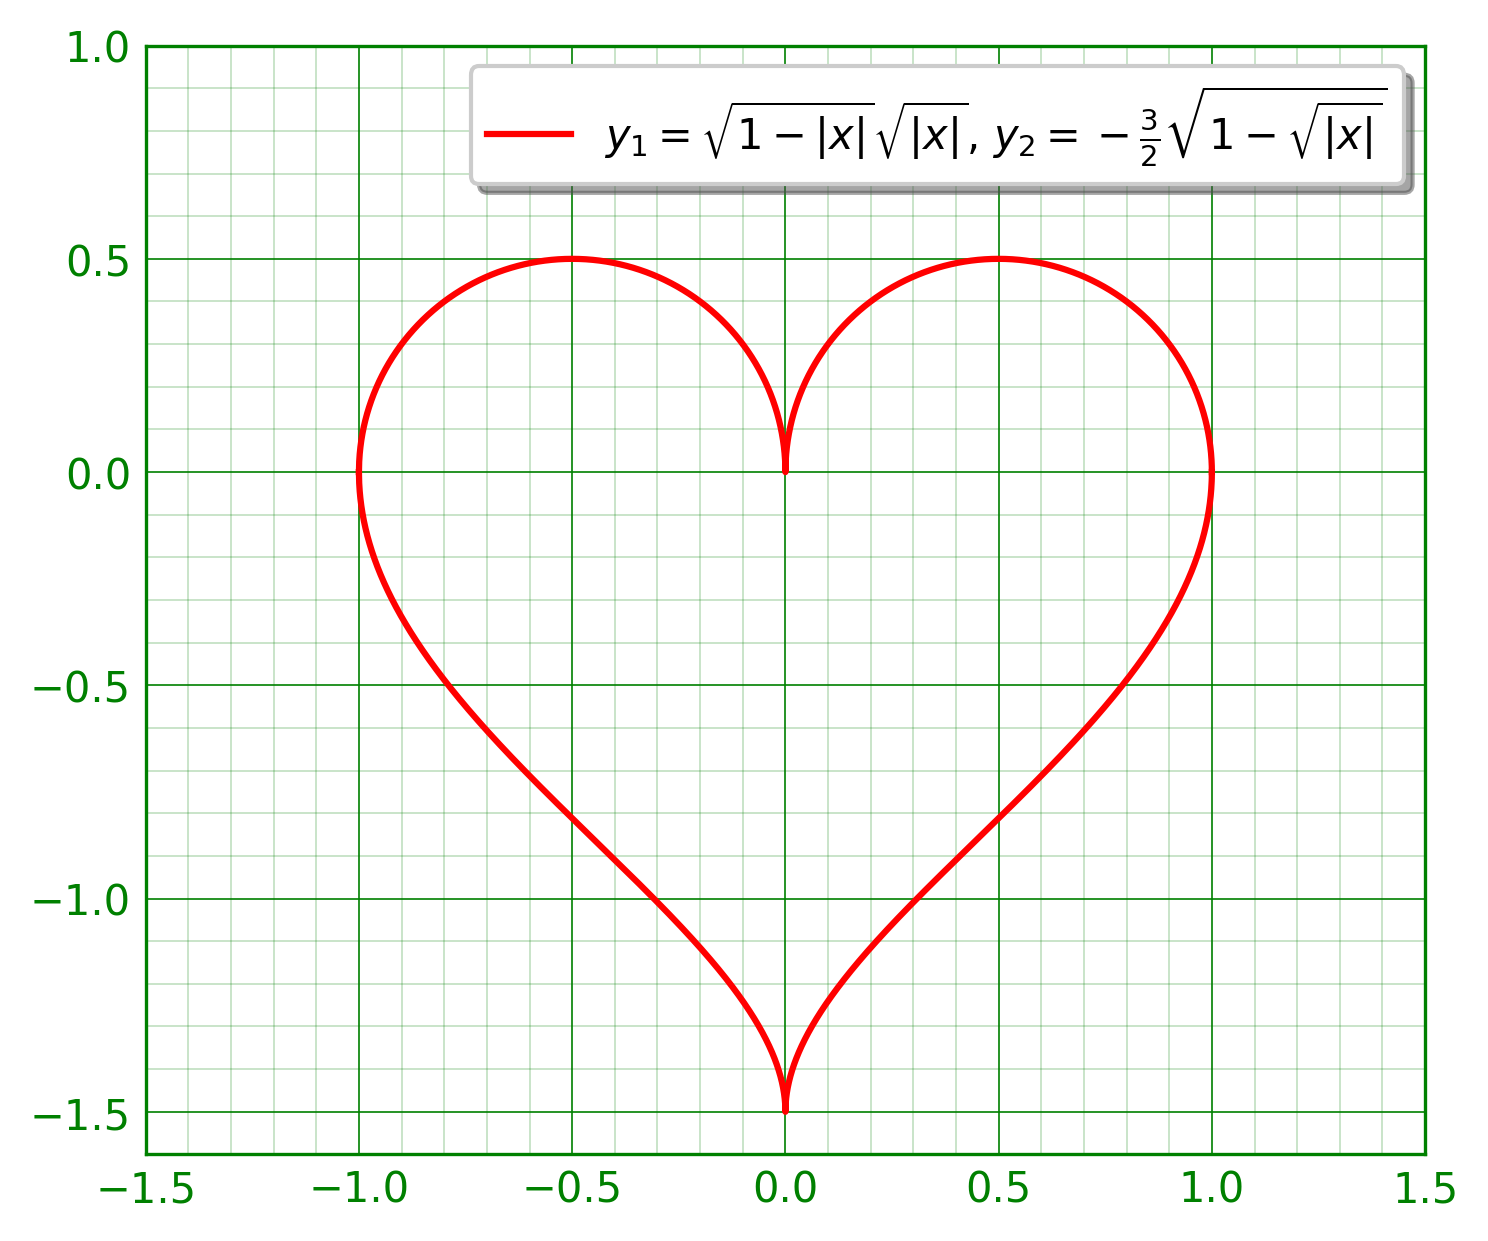
\includegraphics[width=\textwidth]{img/heart-7.png}
        \end{column}
    \end{columns}
\end{frame}


% Heart Plot: Text Message
\begin{frame}[t,fragile]
    \frametitle{Heart Plot: Text Message}
    \vspace{-2mm}
    \begin{columns}[T]
        \begin{column}{0.47\textwidth}
            \pyfile[style=tiny,linerange=30]{examples/heart-8.py}
        \end{column}
        \begin{column}{0.53\textwidth}
            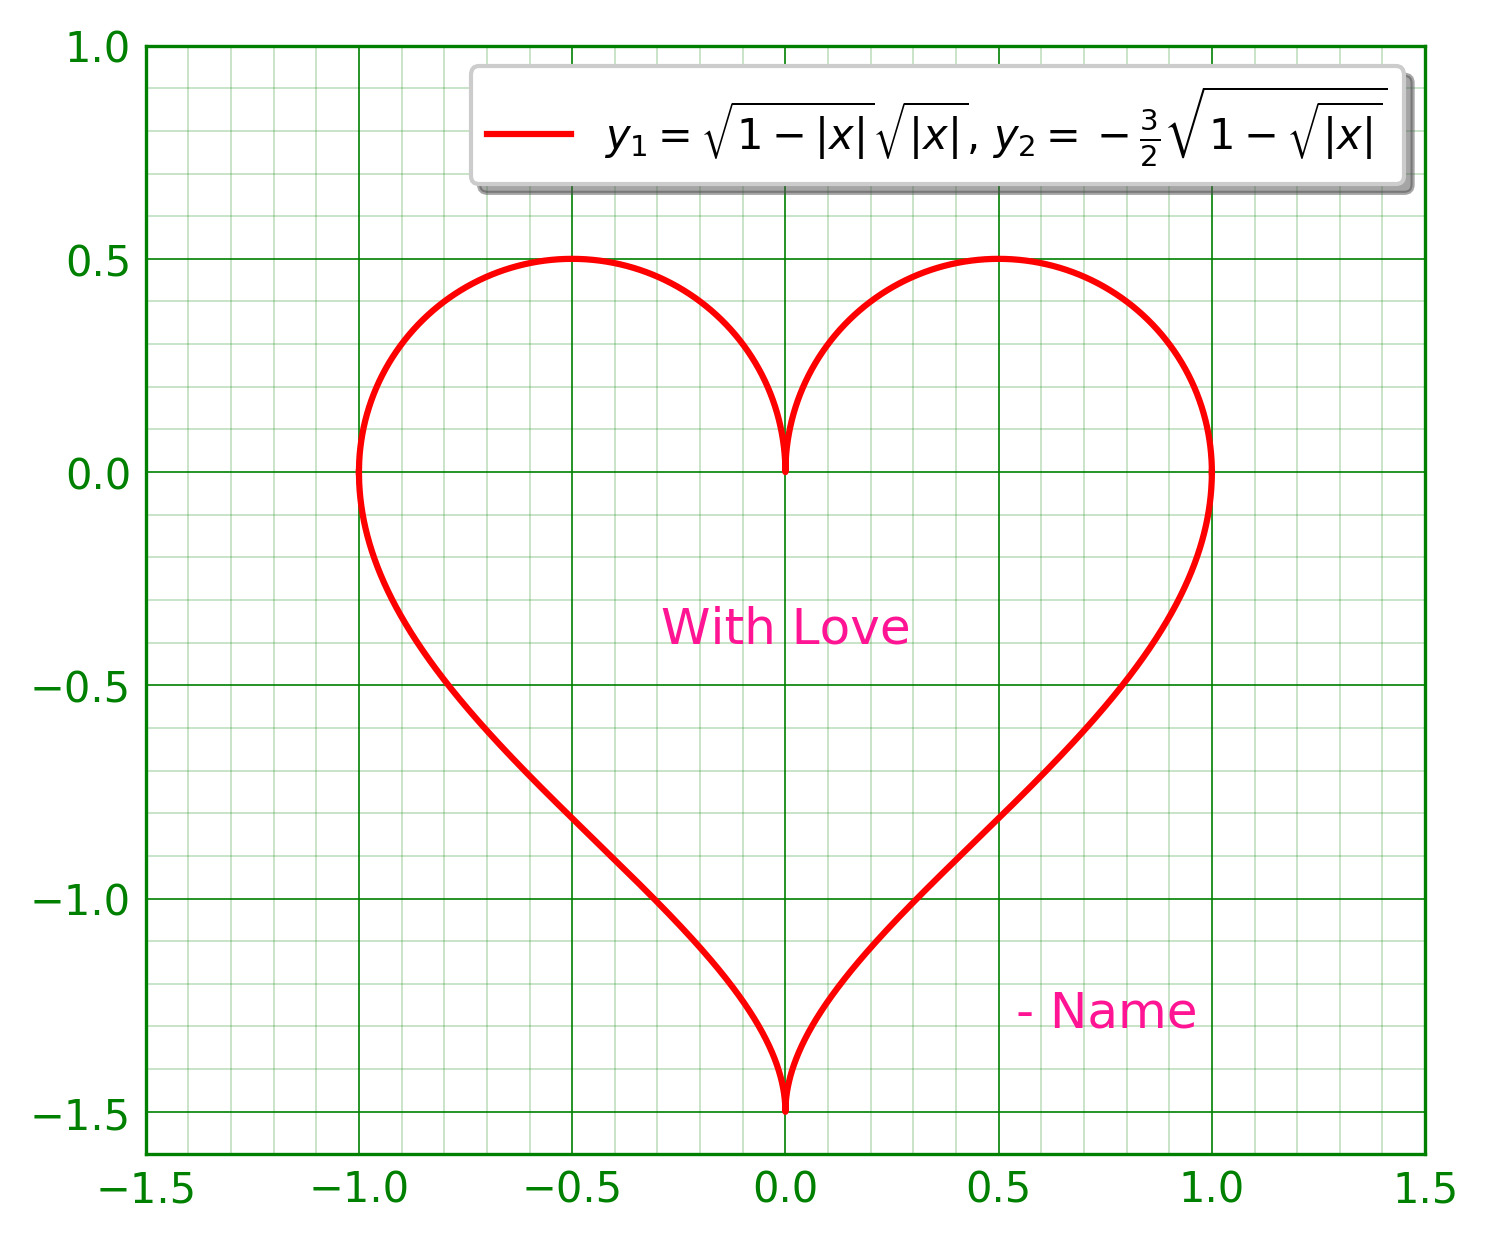
\includegraphics[width=\textwidth]{img/heart-8.png}
        \end{column}
    \end{columns}
\end{frame}


% Regular Plot
\begin{frame}[t,fragile]
    \frametitle{Regular Plot}
    \vspace{-2mm}
    \begin{columns}[T]
        \begin{column}{0.49\textwidth}
            \pyfile[style=footnotesize]{examples/xkcd-0.py}
        \end{column}
        \begin{column}{0.51\textwidth}
            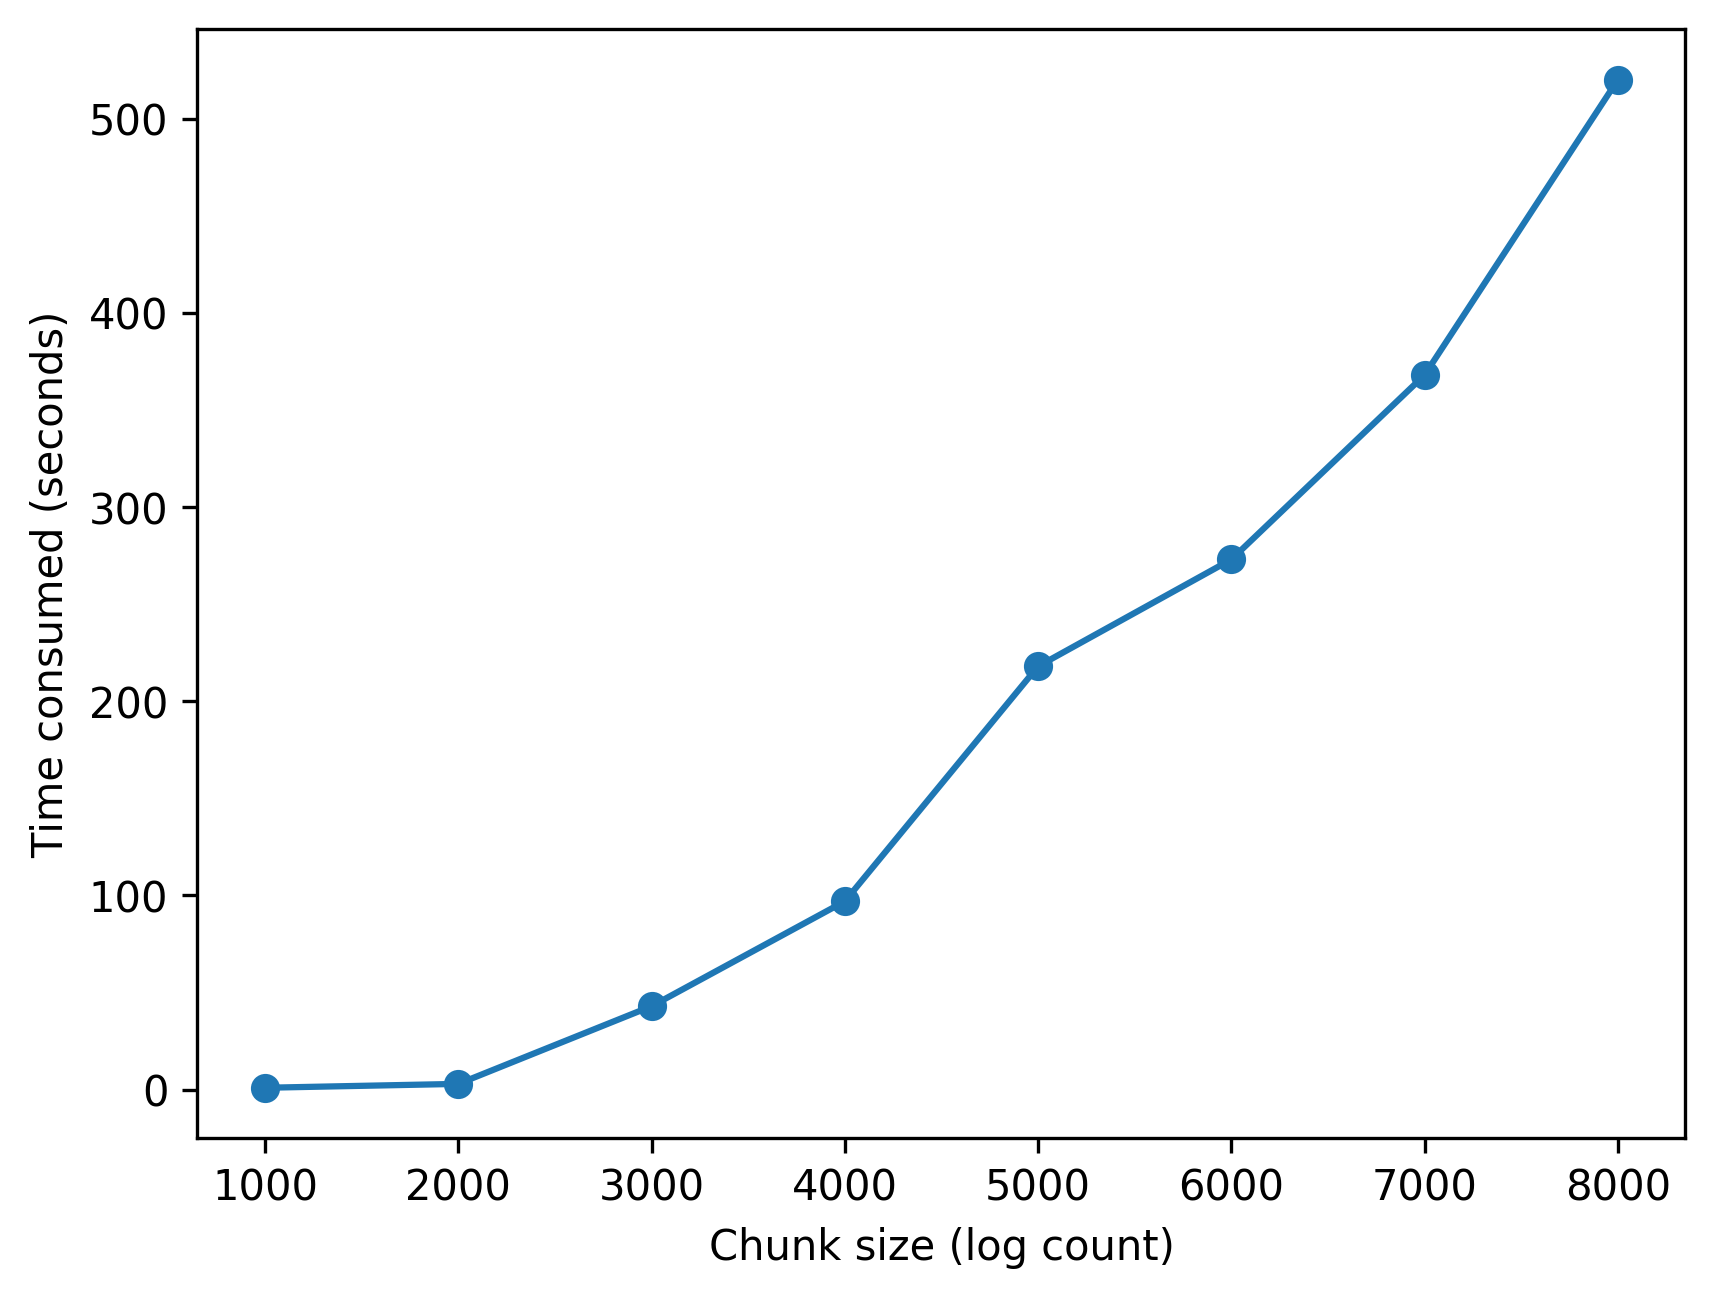
\includegraphics[width=\textwidth]{img/xkcd-0.png}
        \end{column}
    \end{columns}
\end{frame}


% XKCD Plot
\begin{frame}[t,fragile]
    \frametitle{XKCD-Style Plot}
    \vspace{-2mm}
    \begin{columns}[T]
        \begin{column}{0.49\textwidth}
            \pyfile[style=footnotesize]{examples/xkcd-1.py}
        \end{column}
        \begin{column}{0.51\textwidth}
            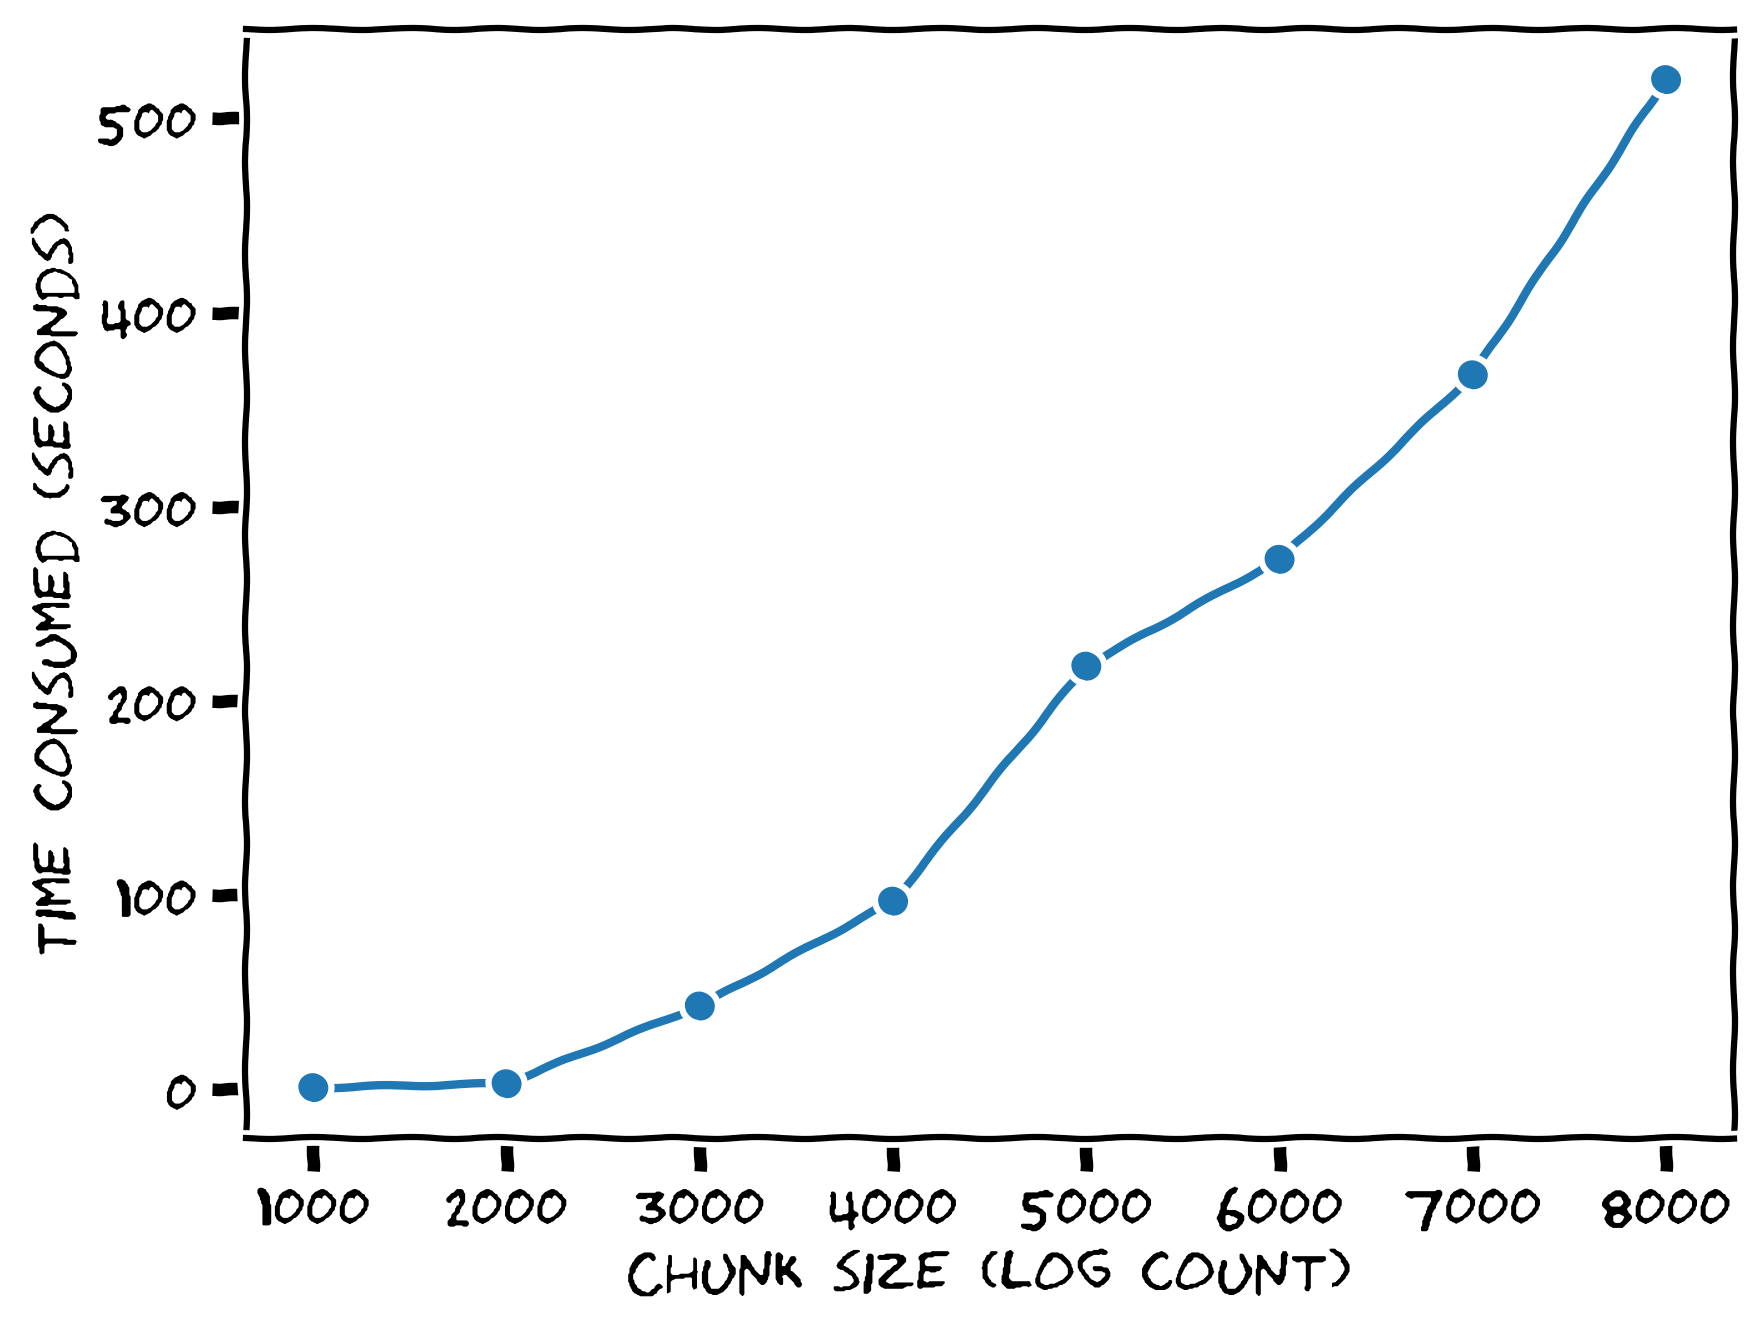
\includegraphics[width=\textwidth]{img/xkcd-1.png}
        \end{column}
    \end{columns}
\end{frame}


% Humor Sans
\begin{frame}[t,fragile]
    \frametitle{XKCD-Style Plot: Font: Humor Sans}

    Install \textbf{Humor Sans} font for best results.

    \medskip

    After installing the font, remove Matplotlib cache \\
    to force rebuilding of font list.

    \medskip

    \begin{shenv}[gobble=8]
        # On macOS
        brew tap homebrew/cask-fonts
        brew cask install font-humor-sans
        rm -rf ~/.matplotlib

        # On Debian, Ubuntu, etc.
        apt-get update
        apt-get install fonts-humor-sans
        rm -rf ~/.cache/matplotlib
    \end{shenv}
\end{frame}


% XKCD Plot: Default Parameters
\begin{frame}[t,fragile]
    \frametitle{XKCD-Style Plot: Default Parameters}
    \vspace{-2mm}
    \begin{columns}[T]
        \begin{column}{0.49\textwidth}
            \pyfile[style=footnotesize]{examples/xkcd-2.py}
        \end{column}
        \begin{column}{0.51\textwidth}
            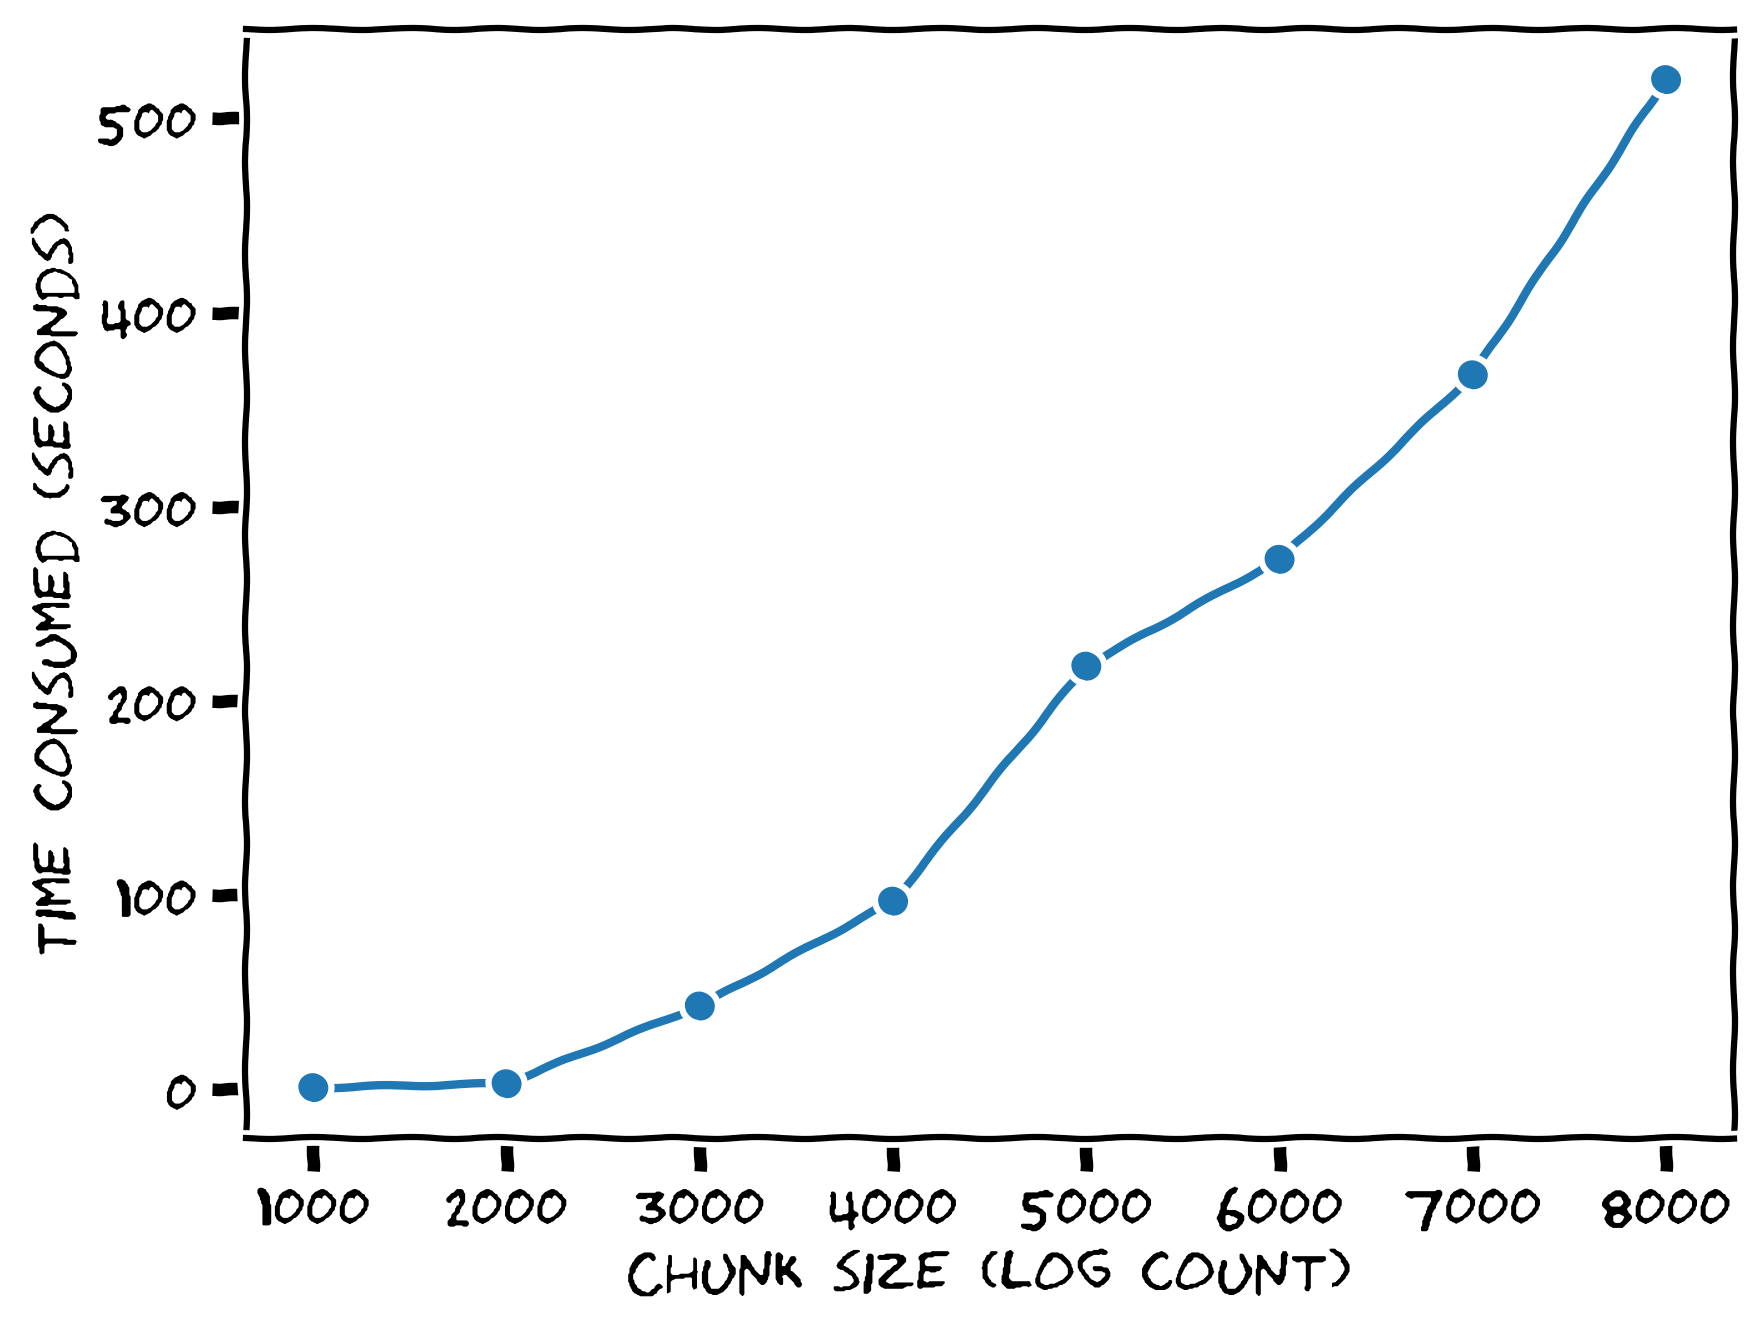
\includegraphics[width=\textwidth]{img/xkcd-1.png}
        \end{column}
    \end{columns}
\end{frame}


% XKCD Plot: scale=5
\begin{frame}[t,fragile]
    \frametitle{XKCD-Style Plot: \texttt{scale=5}}
    \vspace{-2mm}
    \begin{columns}[T]
        \begin{column}{0.49\textwidth}
            \pyfile[style=footnotesize]{examples/xkcd-3.py}
        \end{column}
        \begin{column}{0.51\textwidth}
            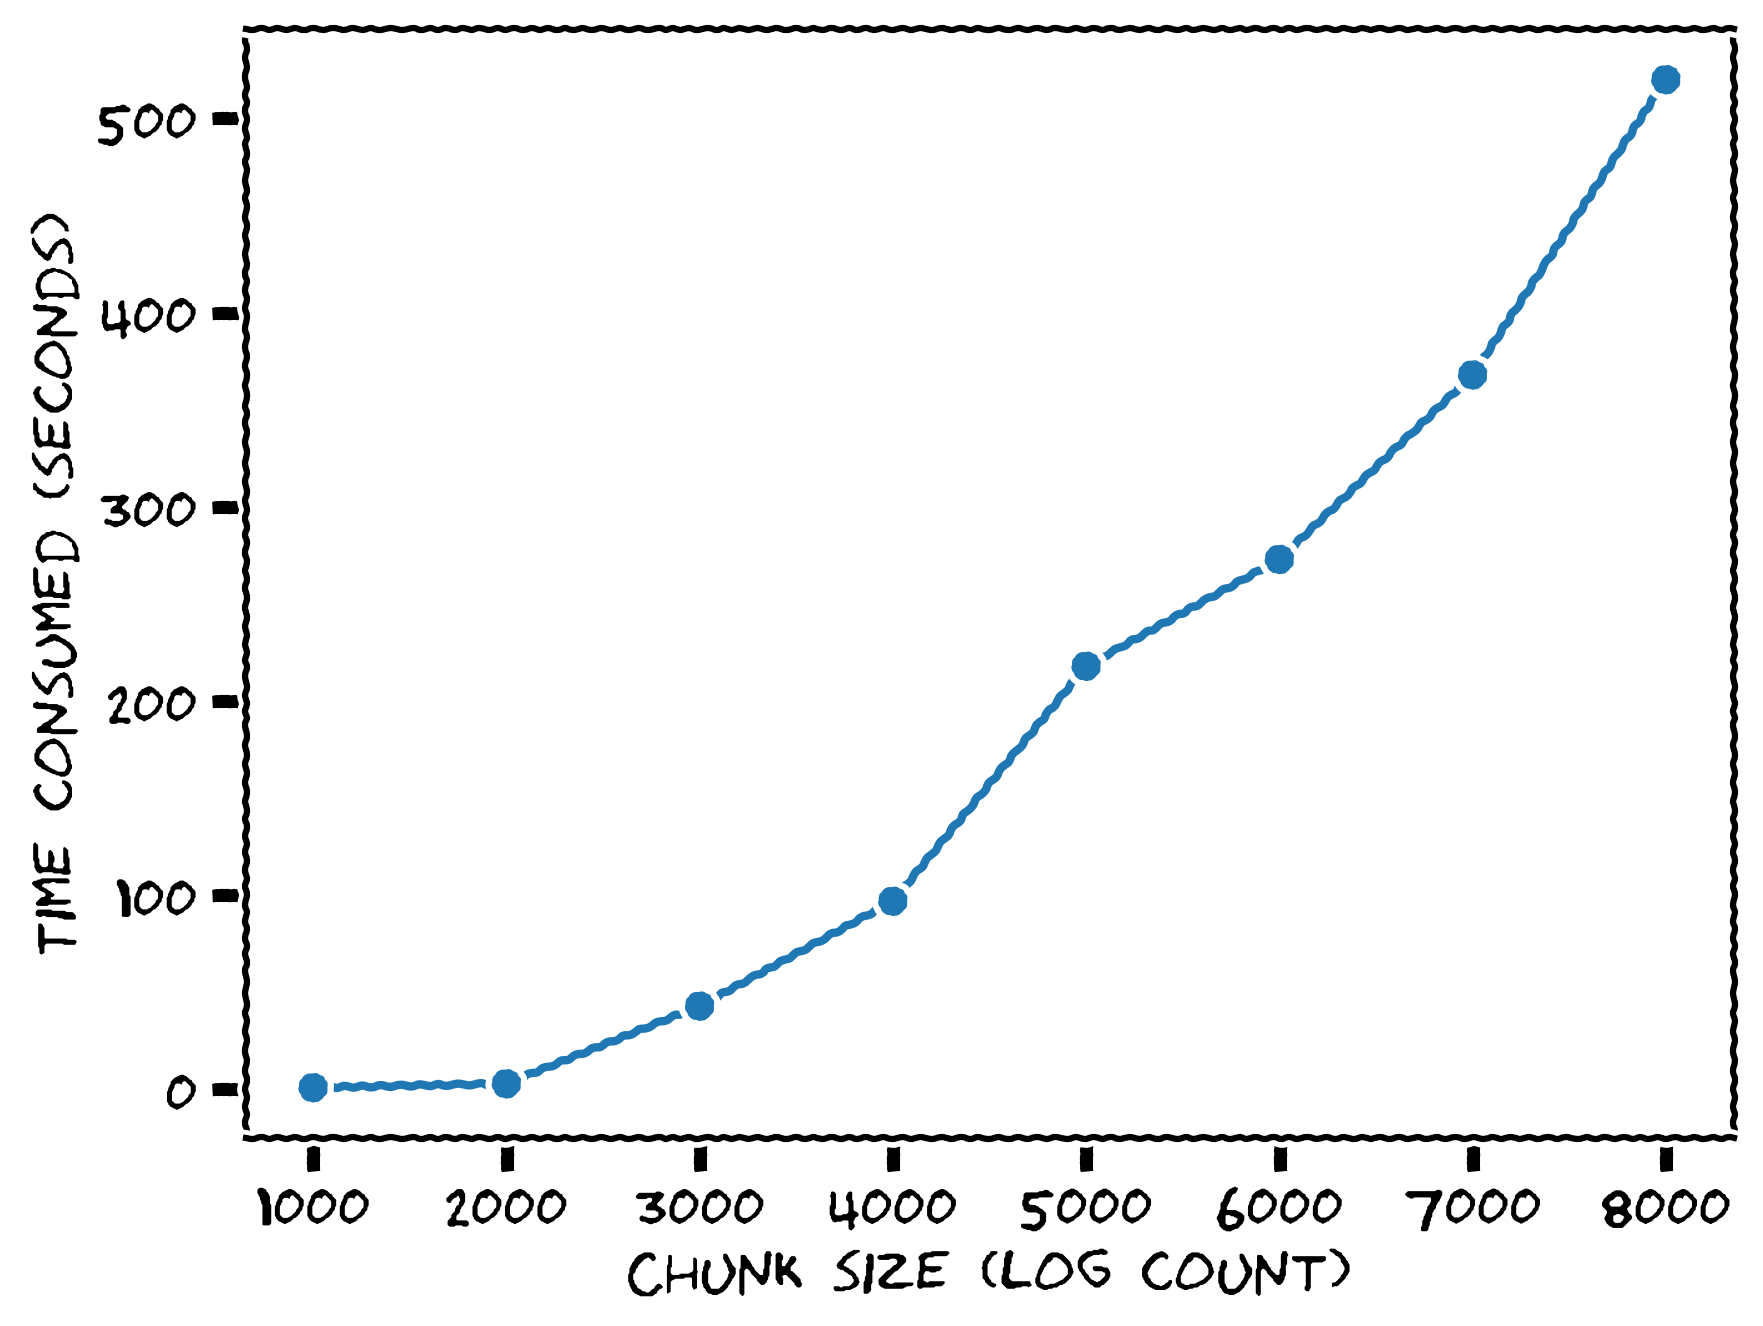
\includegraphics[width=\textwidth]{img/xkcd-3.png}
        \end{column}
    \end{columns}
\end{frame}


% XKCD Plot: scale=0.2
\begin{frame}[t,fragile]
    \frametitle{XKCD-Style Plot: \texttt{scale=0.2}}
    \vspace{-2mm}
    \begin{columns}[T]
        \begin{column}{0.49\textwidth}
            \pyfile[style=footnotesize]{examples/xkcd-4.py}
        \end{column}
        \begin{column}{0.51\textwidth}
            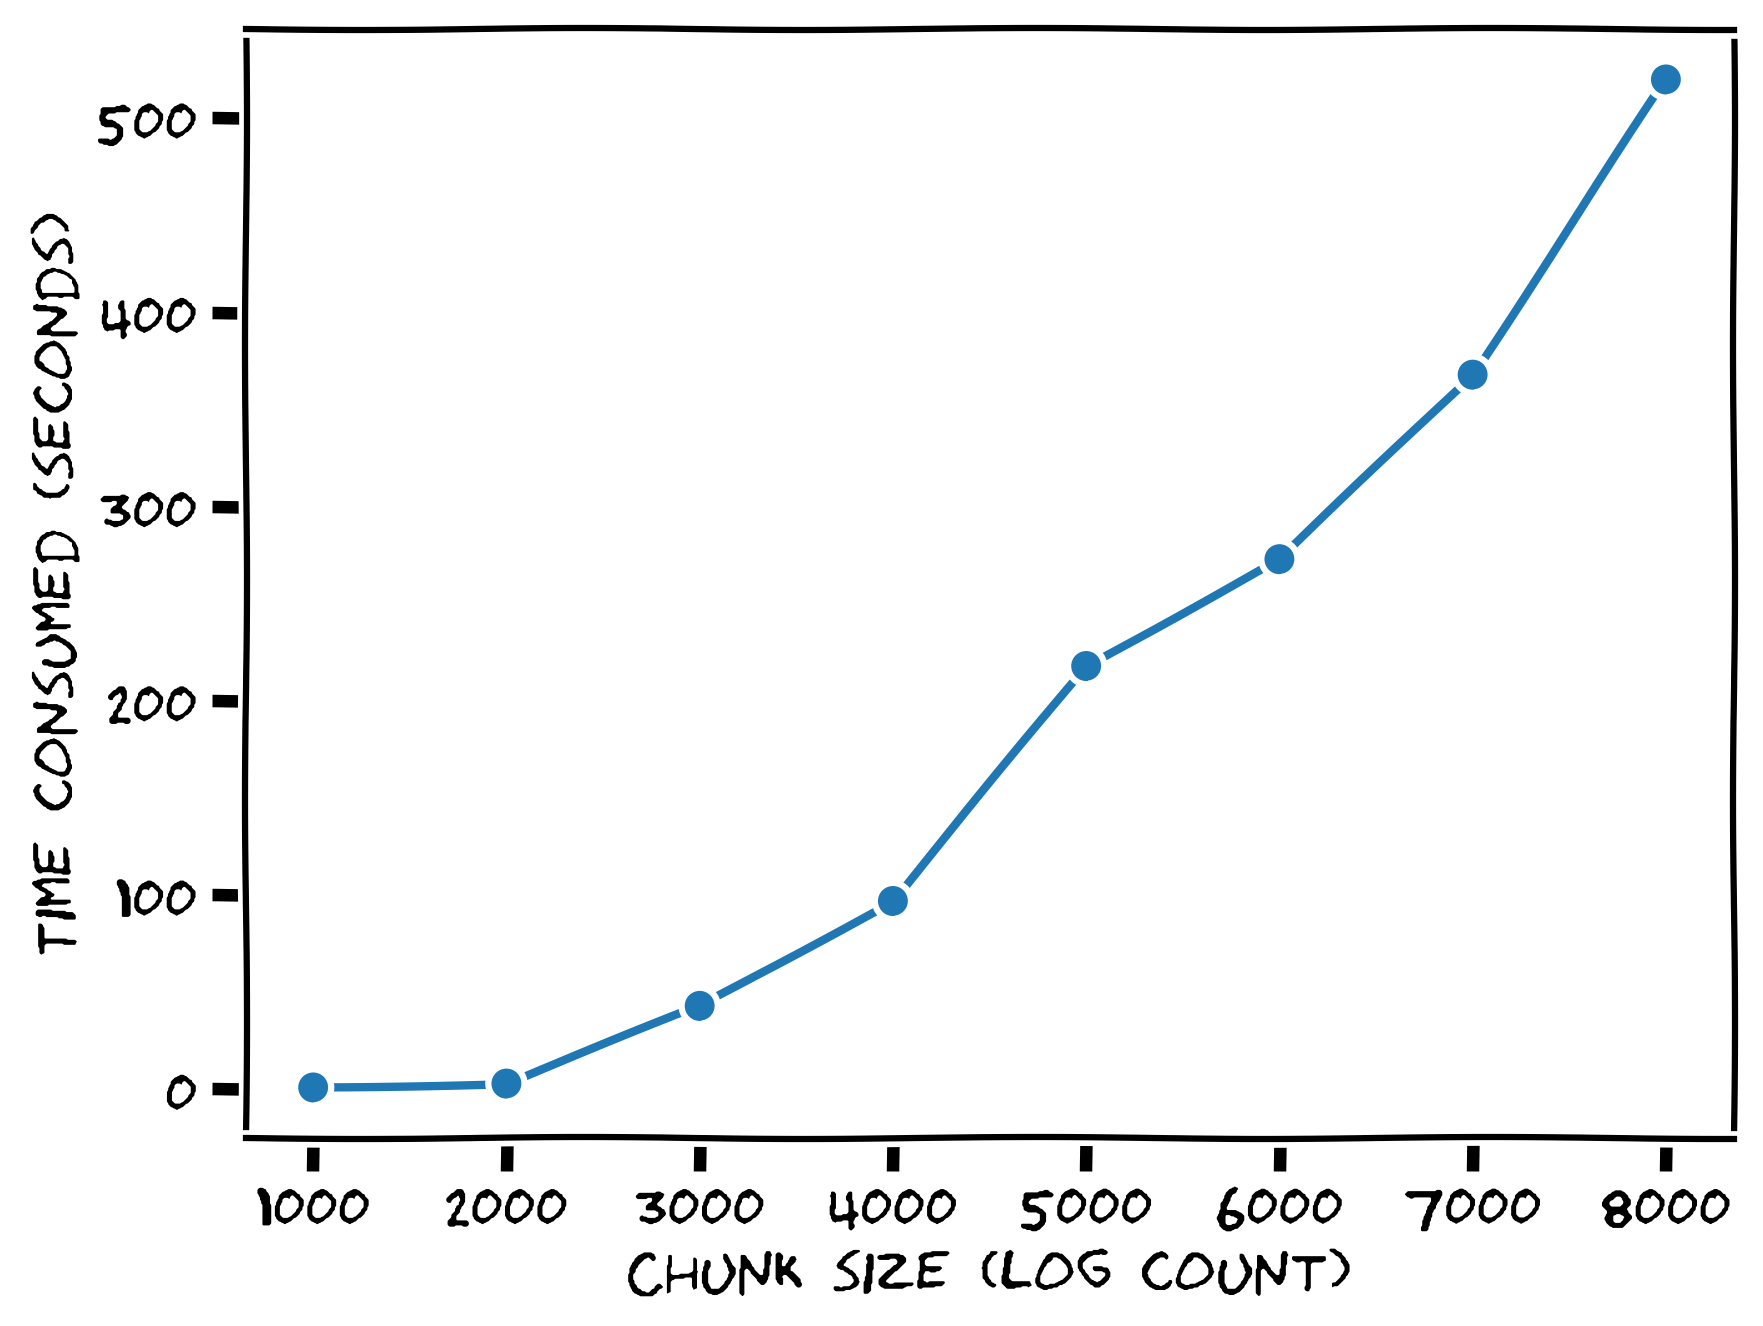
\includegraphics[width=\textwidth]{img/xkcd-4.png}
        \end{column}
    \end{columns}
\end{frame}


% XKCD Plot: length=20
\begin{frame}[t,fragile]
    \frametitle{XKCD-Style Plot: \texttt{length=20}}
    \vspace{-2mm}
    \begin{columns}[T]
        \begin{column}{0.49\textwidth}
            \pyfile[style=footnotesize]{examples/xkcd-5.py}
        \end{column}
        \begin{column}{0.51\textwidth}
            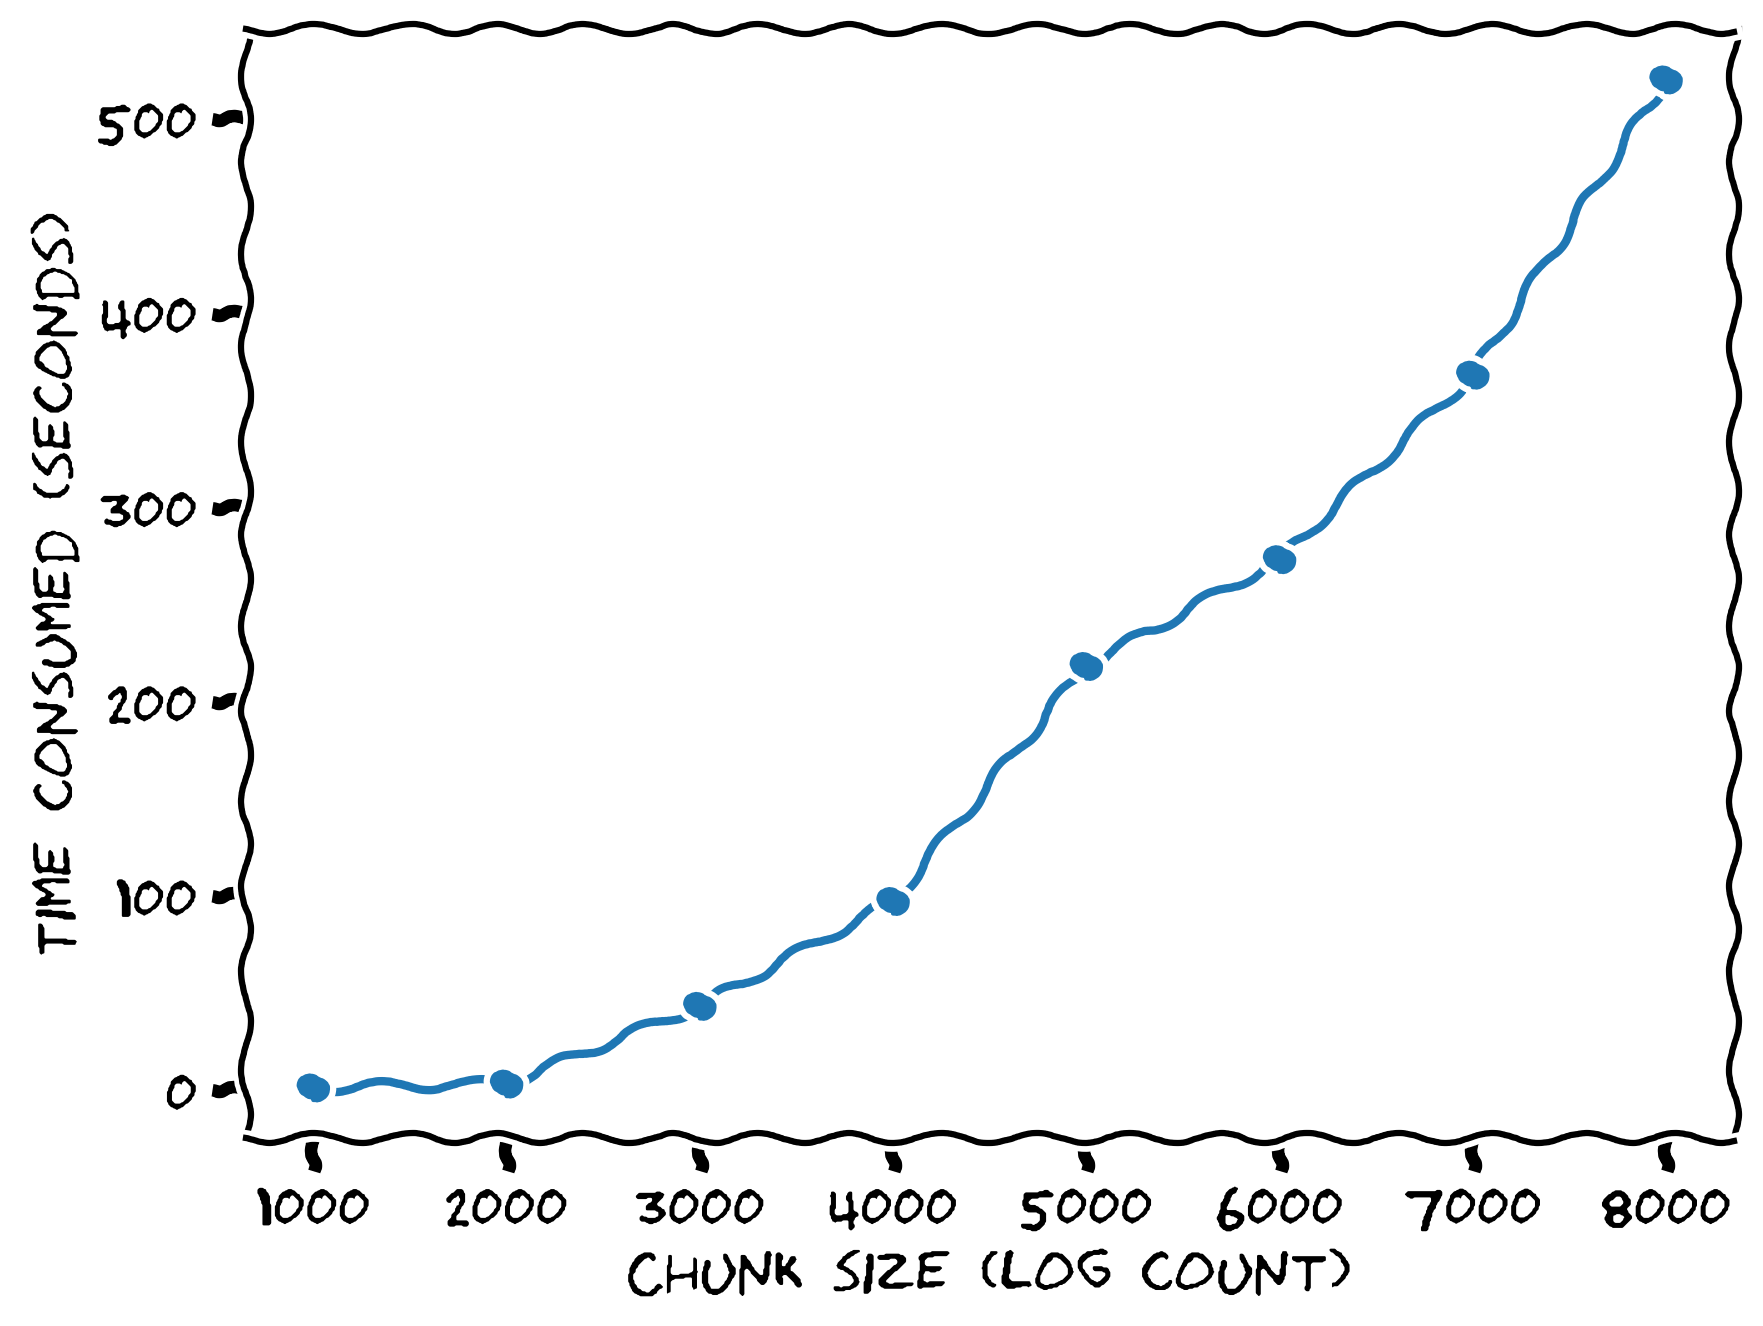
\includegraphics[width=\textwidth]{img/xkcd-5.png}
        \end{column}
    \end{columns}
\end{frame}


% XKCD Plot: length=500
\begin{frame}[t,fragile]
    \frametitle{XKCD-Style Plot: \texttt{length=500}}
    \vspace{-2mm}
    \begin{columns}[T]
        \begin{column}{0.49\textwidth}
            \pyfile[style=footnotesize]{examples/xkcd-6.py}
        \end{column}
        \begin{column}{0.51\textwidth}
            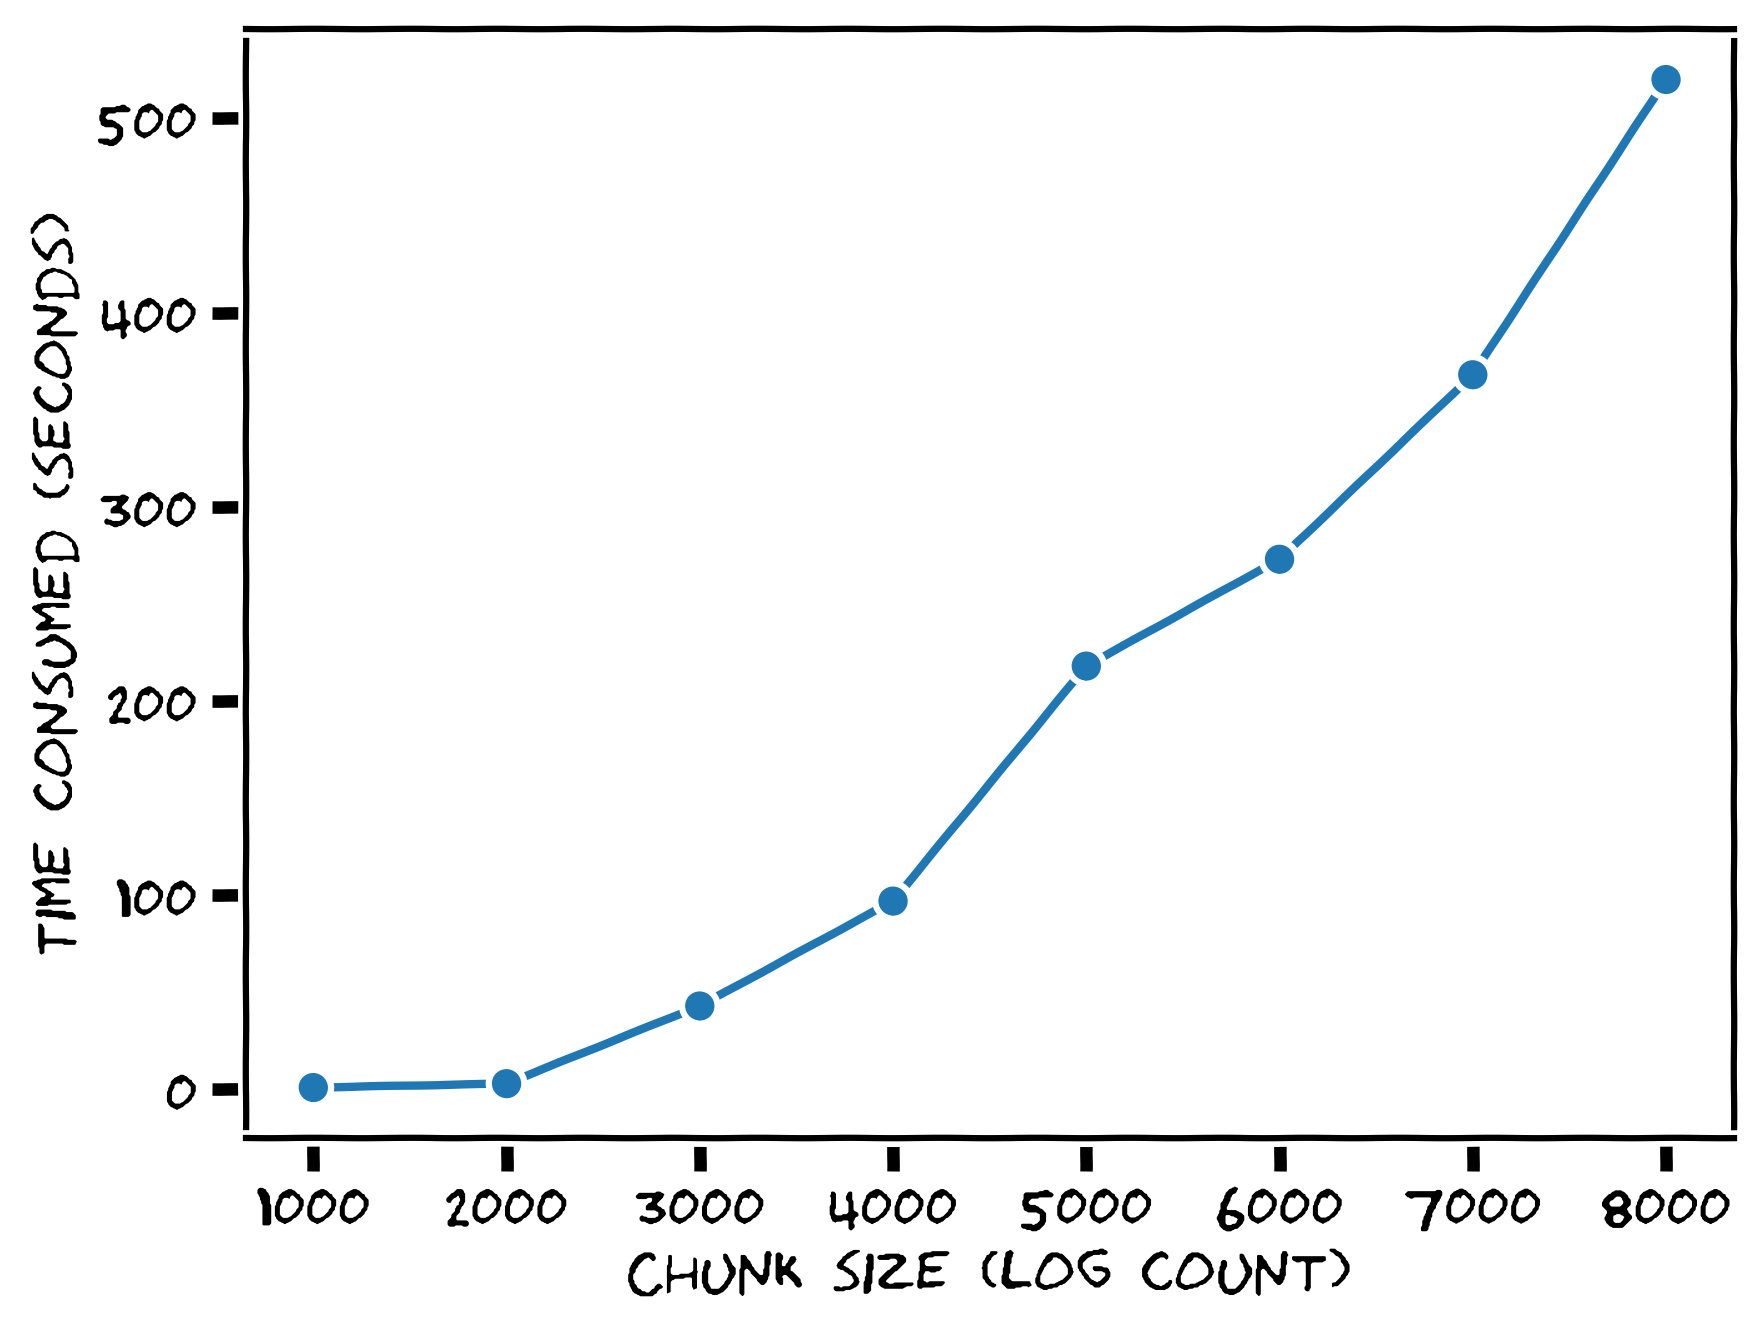
\includegraphics[width=\textwidth]{img/xkcd-6.png}
        \end{column}
    \end{columns}
\end{frame}


% XKCD Plot: randomness=1
\begin{frame}[t,fragile]
    \frametitle{XKCD-Style Plot: \texttt{randomness=1}}
    \vspace{-2mm}
    \begin{columns}[T]
        \begin{column}{0.49\textwidth}
            \pyfile[style=footnotesize]{examples/xkcd-7.py}
        \end{column}
        \begin{column}{0.51\textwidth}
            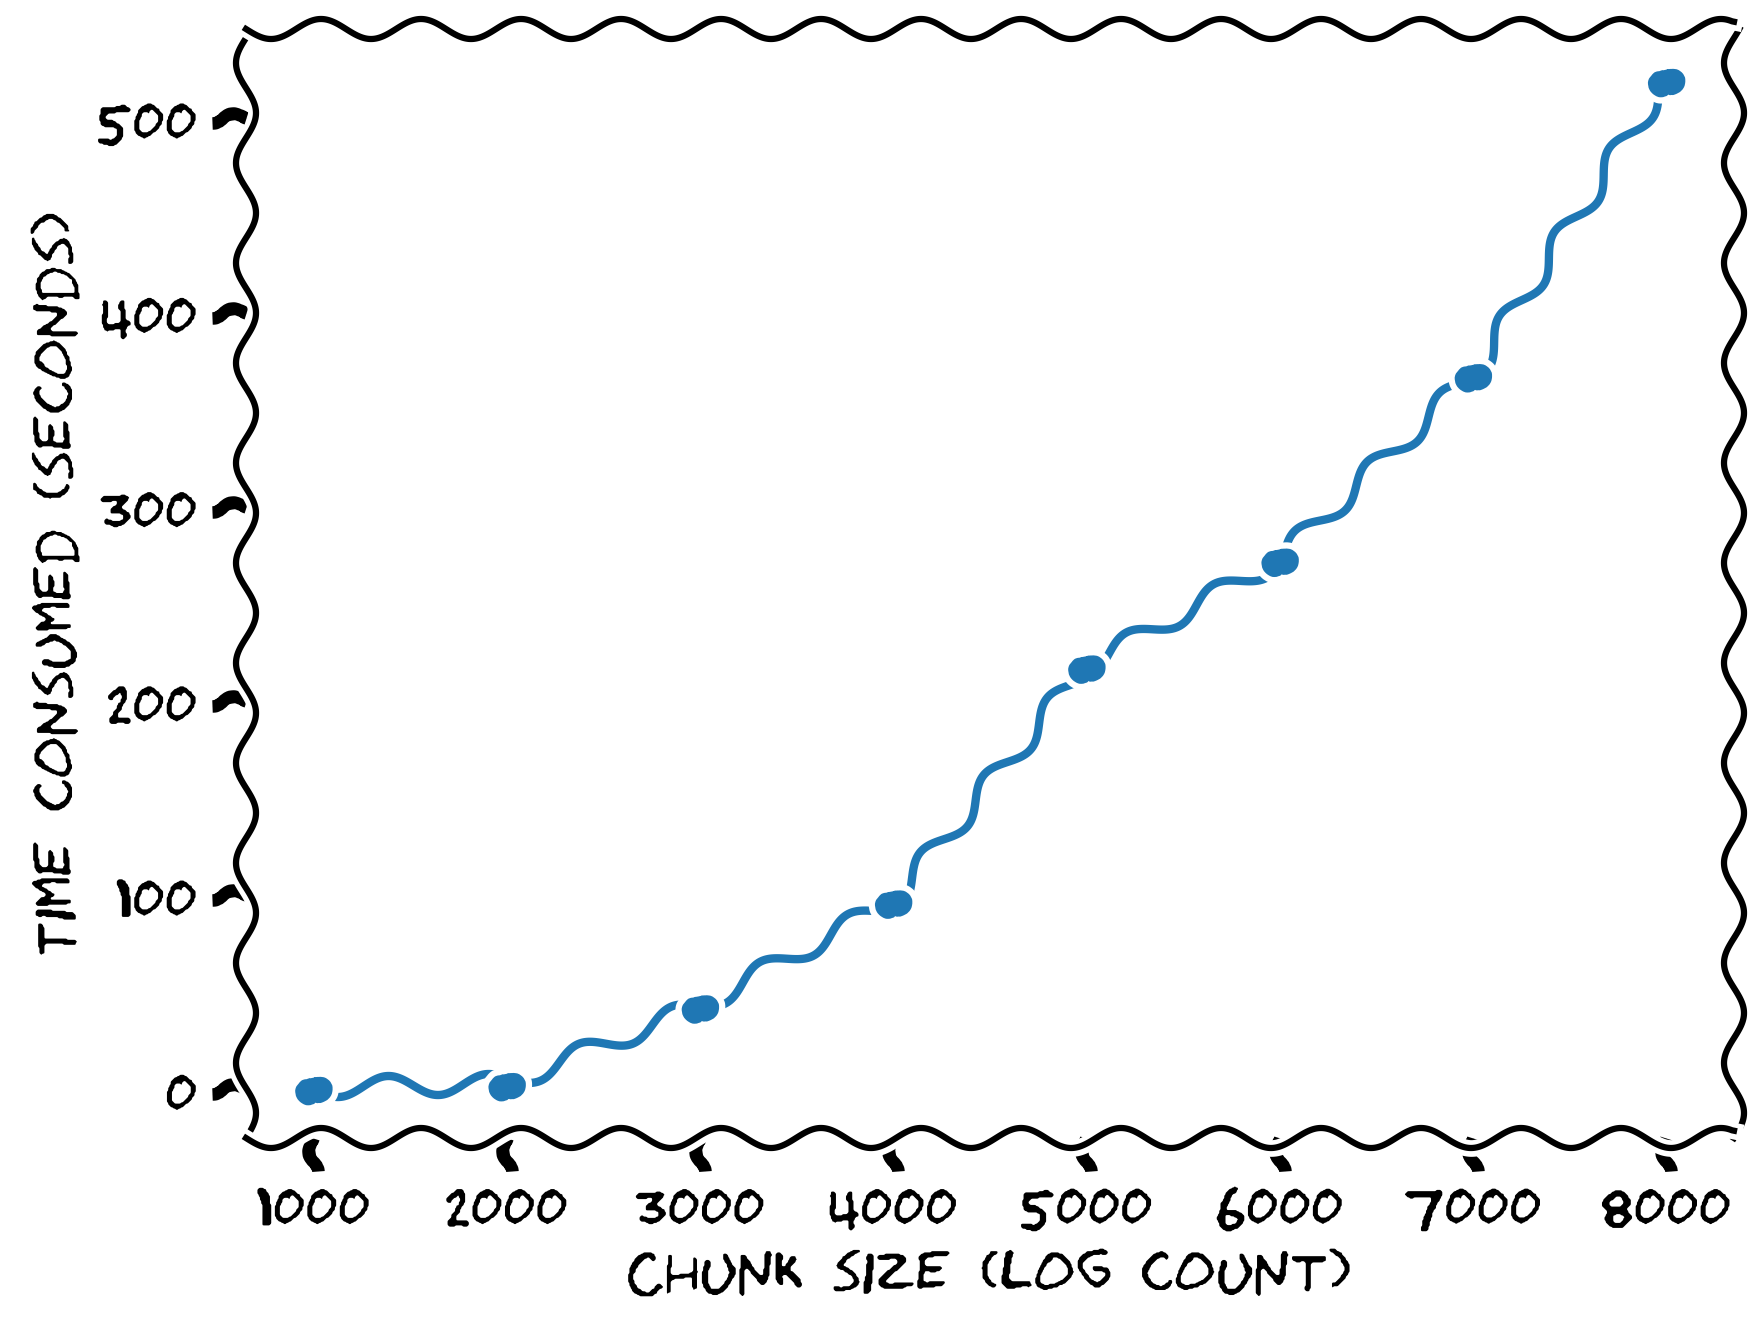
\includegraphics[width=\textwidth]{img/xkcd-7.png}
        \end{column}
    \end{columns}
\end{frame}


% XKCD Plot: randomness=10
\begin{frame}[t,fragile]
    \frametitle{XKCD-Style Plot: \texttt{randomness=10}}
    \vspace{-2mm}
    \begin{columns}[T]
        \begin{column}{0.49\textwidth}
            \pyfile[style=footnotesize]{examples/xkcd-8.py}
        \end{column}
        \begin{column}{0.51\textwidth}
            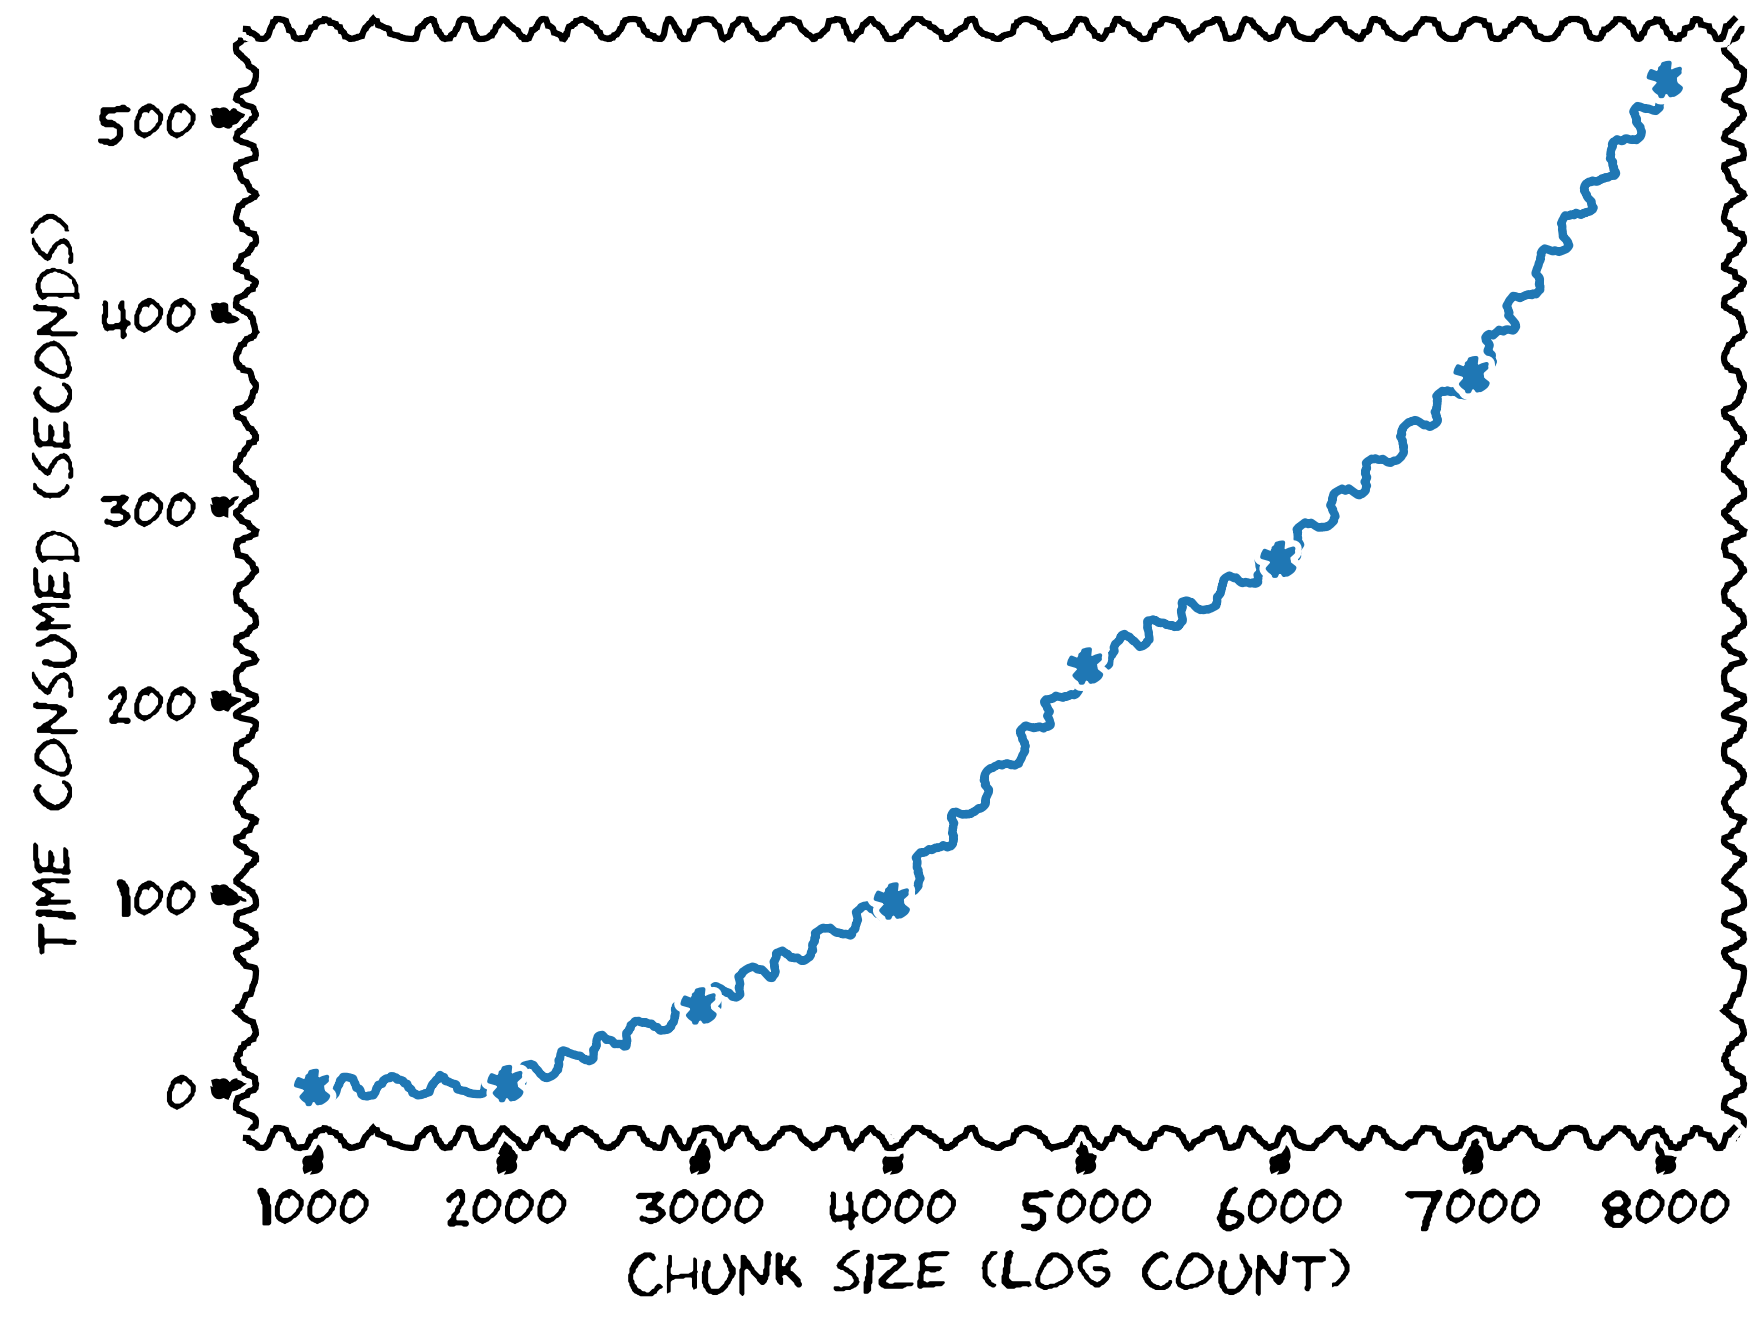
\includegraphics[width=\textwidth]{img/xkcd-8.png}
        \end{column}
    \end{columns}
\end{frame}


% Thank You!
\begin{frame}
    \Huge
    \centering

    Thank You
\end{frame}

\end{document}
